\documentclass[../../main.tex]{subfiles}
\begin{document}

\setcounter{footnote}{0} 


\section{Manuscript I}
\emph{Rationalizing the Activity of an “Artificial Diels-Alderase”: Establishing Efficient and Accurate Protocols for Calculating Supramolecular Catalysis}


\subsection{Abstract}

Self-assembled cages have emerged as novel platforms to explore bio-inspired catalysis. While many different size and shape supramolecular structures are now readily accessible, only a few are known to accelerate chemical reactions under sub-stoichiometric conditions. These limited examples point to a poor understanding of cage catalysis in general, limiting the ability to design new systems. Here we show that a simple and efficient density functional theory-based methodology, informed by explicitly solvated molecular dynamics and coupled cluster calculations is sufficient to accurately reproduce experimental guest binding affinities (MAD = 1.9 \kcal) and identify the catalytic Diels-Alder proficiencies ($>$80 \% accuracy) of two homologous Pd$_2$L$_4$ metallocages with a variety of substrates. This analysis reveals how subtle structural differences in the cage framework affect binding and catalysis. These effects manifest in a smaller distortion and more favourable interaction energy for the catalytic cage compared to the inactive structure. This study gives a detailed insight that would otherwise be difficult to obtain from experiments, providing new opportunities in the design of catalytically active supramolecular cages.


\subsection{Introduction}

Self-assembly of molecular building blocks is ubiquitous in nature. Examples of this appear in protein cages,\cite{Theil2011, Azuma2016} enzyme complexes,\cite{Schmitt2017} and bacterial nanocompartments.\cite{Rurup2014} The remarkable properties of these structures have inspired the design of biomimetic systems that exhibit similar properties at a minimalistic scale. In this context, a large variety of self-assembled cages constructed from simple building blocks via metal–ligand interactions,\cite{Wiester2011, Cook2013} hydrogen bonds,\cite{Pahima2019, Zhang2013, Ajami2013} and other non-covalent interactions\cite{Kaanumalle2005} have been reported in recent decades. 

While many cages have been used successfully for recognition and sensing, far fewer have mimicked the catalytic proficiency and selectivity observed in enzymes. More than twenty years have passed since Sanders raised the question regarding the scarcity of effective supramolecular catalysts.\cite{Sanders1998} Still, his words remain a timely reminder of both the challenges and opportunities within this field. To date, only a handful of self-assembled catalytic metallocages exist,\cite{Fang2019} most notably the [Ga$_4$L$_6$]$^{12-}$ tetrahedron originally developed by Raymond.\cite{Caulder1998} Through a fruitful collaboration with Bergman and recently Toste, this water-soluble anionic assembly has been shown to catalyse a number of transformations, including aza-Cope\cite{Fiedler2004, Brown2009} and Prins rearrangements,\cite{HartCooper2015, Kaphan2015}, the Nazarov cyclisation,\cite{Hastings2010} and hydrolysis of acid-labile compounds under basic conditions,\cite{Pluth2007} among others.\cite{Fang2019} The prototypical self-assembled metallocages developed in Makoto Fujita's group have also been shown to catalyse Diels-Alder and Knoevenagel reactions,\cite{Yoshizawa2006, Murase2011} while other water soluble systems can promote different hydrolysis reactions.\cite{Bolliger2013, Cullen2016, Cullen2018} Several trends have emerged from these investigations. First, substrate encapsulation occurs due to the hydrophobic effect. Second, many of the reactions produce water soluble products to avoid inhibition. Thirdly, acceleration is commonly a consequence of high effective concentration of substrates or functional groups, either through co-encapsulation, ion-pairing or constrictive binding, and/or coulombic interactions between the charged host and electrostatically matched intermediates.\cite{Chakraborty2019, Goehry2015} These approaches while effective in providing acceleration, in many cases suffer from product inhibition (turnover) or are specific to water-soluble cages. 
Despite notable examples of cage-catalysis, there has been a distinct lack of complementary computational investigation, probably due to their large size and the presence of multiple metal centres. Indeed, only recently, the catalytic activity of the [Ga$_4$L$_6$]$^{12–}$ cage has been explored computationally by Head-Gordon and Ujaque, respectively.\cite{VaissierWelborn2018, Norjmaa2019} Other catalytic activity studies have almost exclusively focused on organic systems.\cite{Pahima2019, Chakraborty2019, Goehry2015, Daver2017, Daver2018} In this work, we focus on the [Pd$_2$L$_4$]$^{4+}$ architecture, which occupies a prominent place in supramolecular chemistry.\cite{Lewis2012, Schmidt2014, Preston2016, Vasdev2017, Preston2017} Originally reported by Steel and co-workers,\cite{McMorran1998} the [Pd$_2$L$_4$]$^{4+}$ topology is one of the simplest and most versatile architectures.\cite{Schmidt2014, Vasdev2017} To date, several homo- and heteroleptic variants (consisting of one or different types of ligand, respectively) have been reported by Hooley,\cite{Liao2010} Shionoya,\cite{Clever2009} Clever,\cite{Bloch2017, Zhu2018, Li2019, Chen2019} Crowley,\cite{Lewis2013, McNeill2015} and others,\cite{Jansze2017, Chand2001, Kishi2011} with applications in molecular recognition,\cite{Kishi2011} drug delivery,\cite{Lewis2012} stabilization of reactive species,\cite{Yamashina2014} and recently catalysis.\cite{MartCentelles2018} Despite their promising applications and scope for redesign, no computational investigation has been carried out to explore their catalytic power. The few prior computational studies on this system have only focused on structural\cite{Preston2016} and spectroscopic analysis.\cite{Schmidt2016} 

In 2018, Lusby and co-workers evaluated the ability of simple [Pd$_2$L$_4$]$^{4+}$ capsules C-1\\ ([Pd$_2$L$^{\text{CH}}_4$]$^{4+}$) and C-2 [Pd$_2$L$^{\text{N}}_4$]$^{4+}$) to catalyse Diels-Alder (DA) reactions, using quinone substrates as dienophiles in dichloromethane (DCM) solvent at room temperature (Figure \ref{fig::da_1}).\cite{MartCentelles2018} Unlike most other capsule-catalysed reaction, this method principally exploits enthalpic activation, where C–H hydrogen bond interactions were postulated to activate the dienophile. It was observed that while C-2 was catalytic (rate accelerations ($k_\text{cat}/k_\text{uncat}$) of up to $10^3$), the homologous C-1 cage was inactive, despite C-1 binding quinones in the same mode. The contrasting catalytic ability was postulated to arise as a result of two factors: weakened substrate binding in C-2 due to a repulsive interaction in the ground-state between the nitrogen lone pair ($n$) and the $\pi$-bond of the guest, and stabilization of the TS through the formation of favourable N$\cdots$HC hydrogen bonds. The latter was inferred from the stronger binding of a TS mimic (the DA adduct of benzoquinone and cyclopentadiene) in C-2 compared to C-1.\cite{MartCentelles2018} However, the difference in catalysis has been purely rationalized on the basis of thermodynamic parameters, such that the precise origin of acceleration, and by extension lack of activity for C-1, are still poorly understood. This substantially limits our ability to design supramolecular catalysts for new chemical reactions. 

\begin{figure}[h!]
	\vspace{0.4cm}
	\centering
	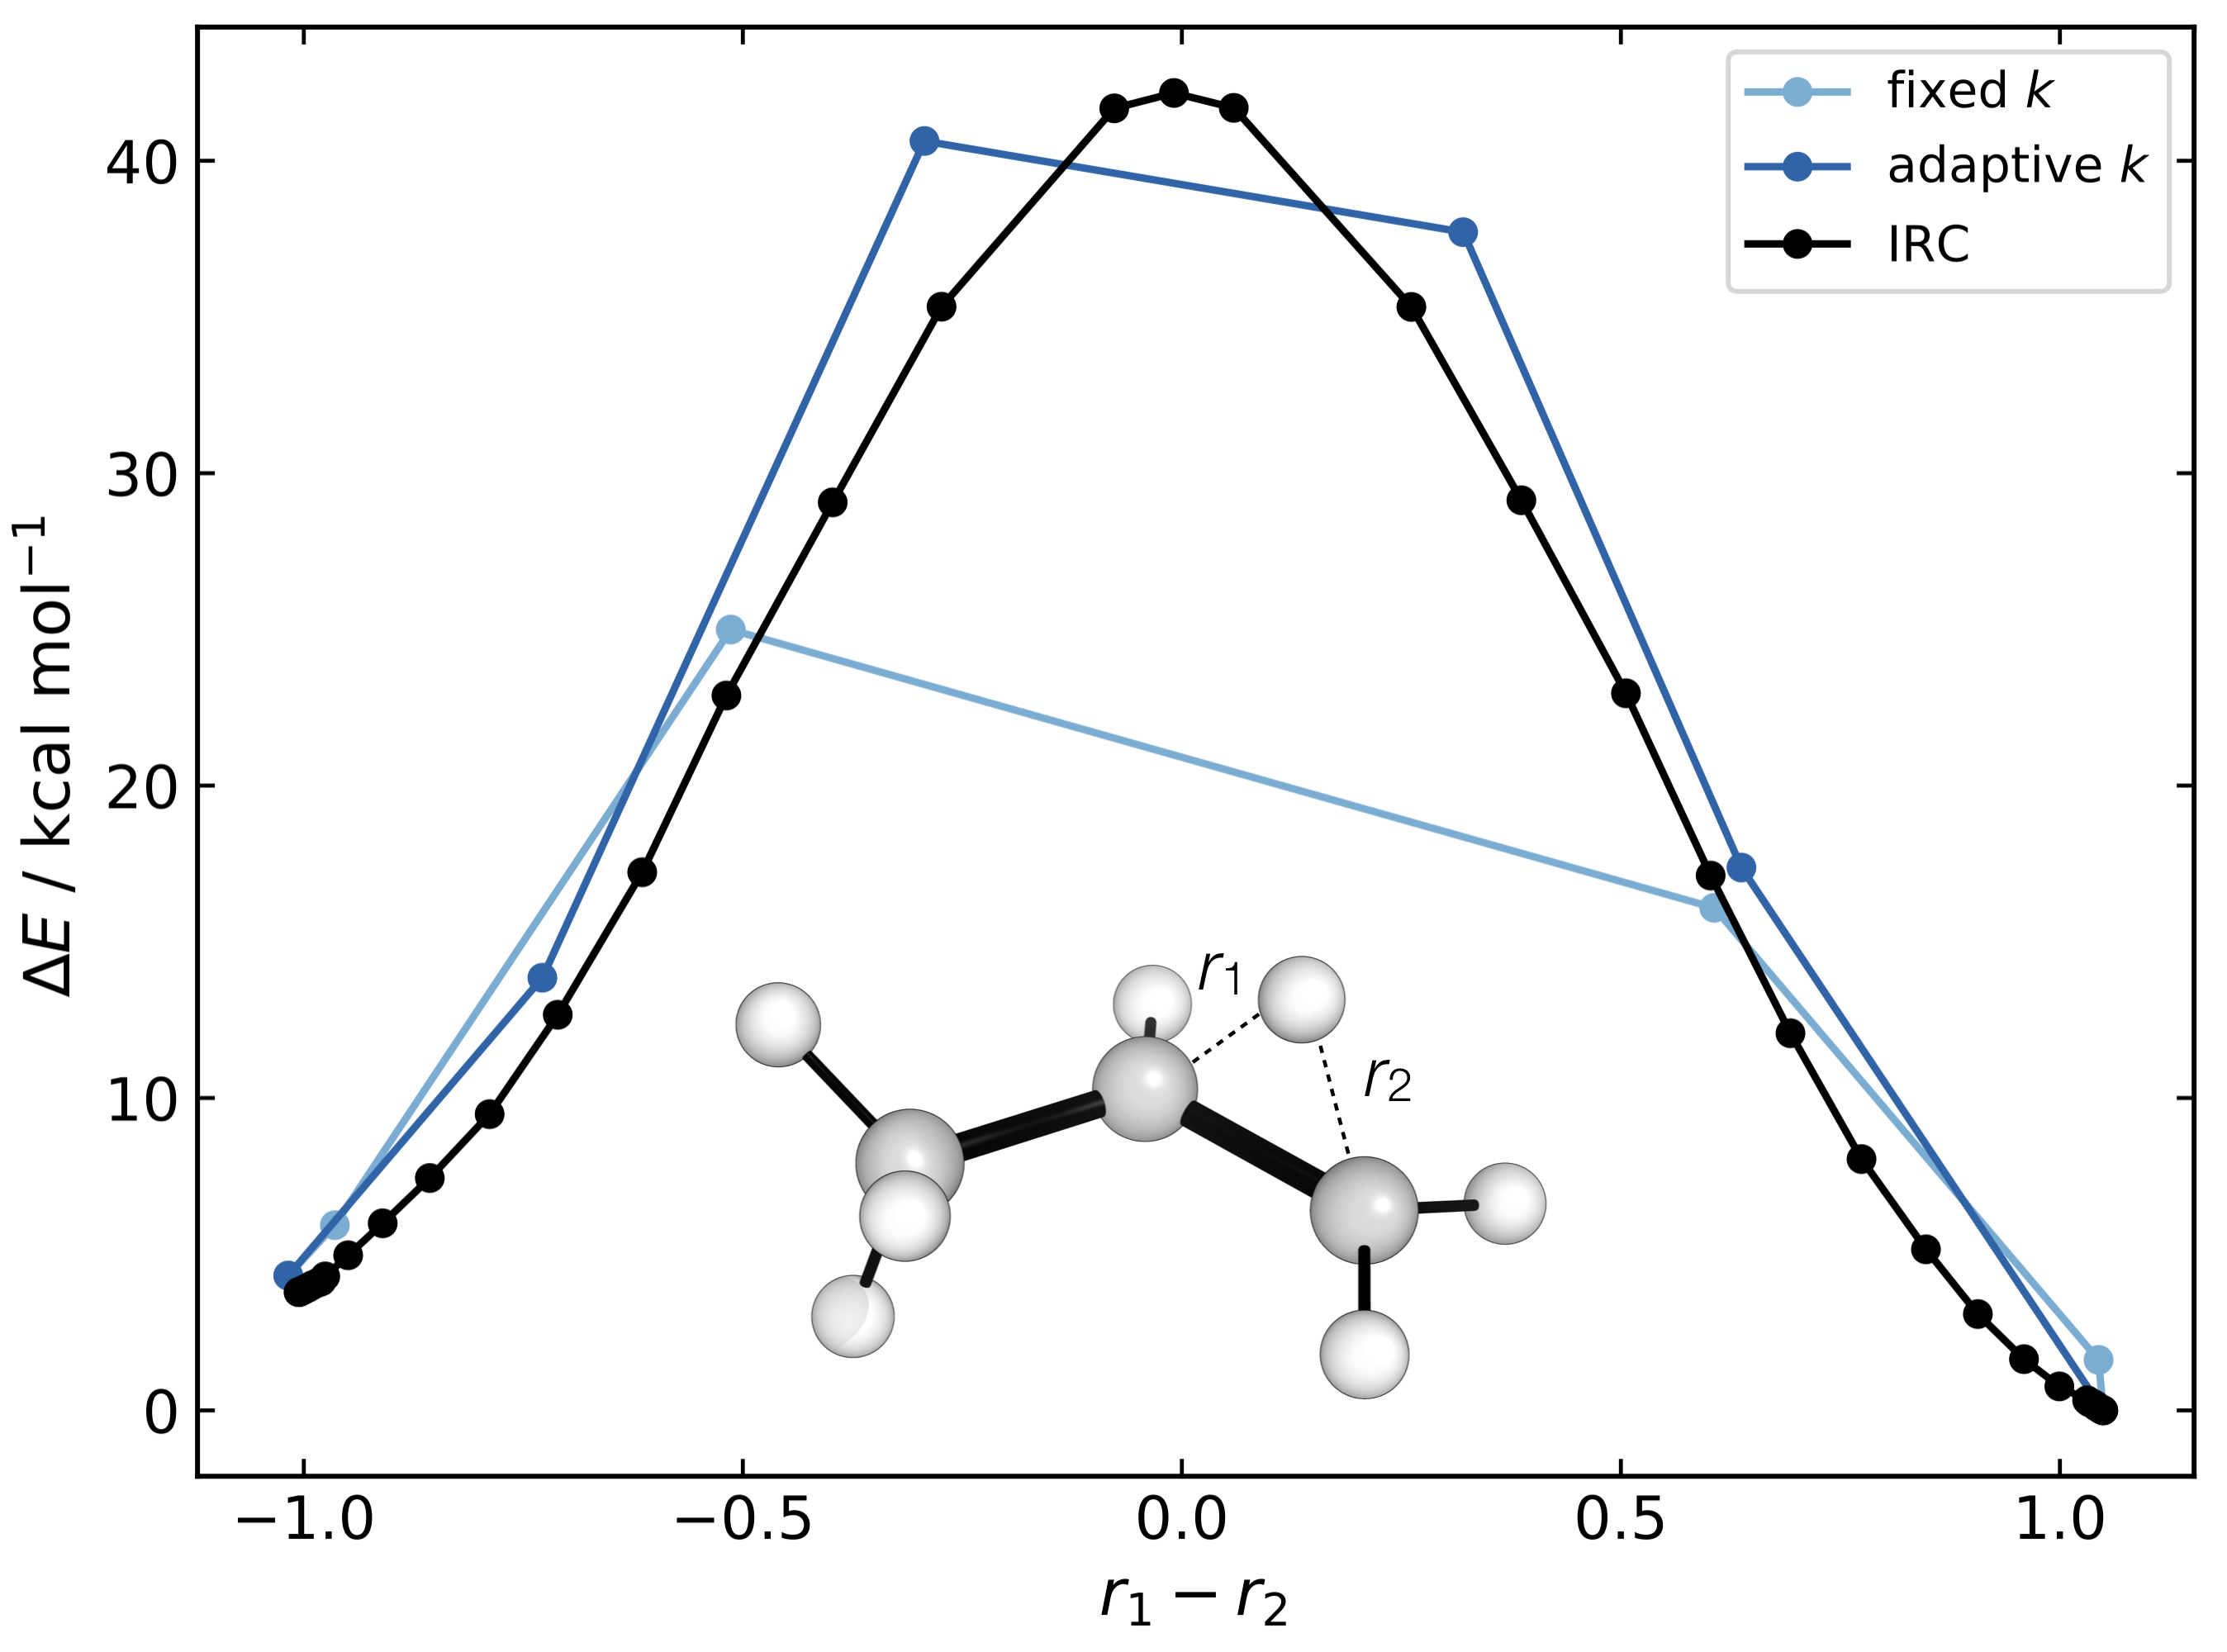
\includegraphics[width=10cm]{3/da//figs/fig1/fig1}
	\vspace{0.2cm}
	\hrule
	\caption{(a) Diels-Alder reaction studied by Lusby and co-workers employing the [Pd2L4]2+ capsules, C-1 and C-2. (b) Schematic representation of our computational approach.}
	\label{fig::da_1}
\end{figure}

Computational studies that could quantitatively rationalize such observations are highly desirable to optimize and design of novel catalytic cages. However, the ability to routinely study and predict binding and catalysis in solution remains an open challenge. This is particularly true for the latter, where both thermodynamic and kinetic aspects must be considered. In this context, this work aims to rationalize the observed differences in binding and catalysis between metallocages C-1 and C-2, paving the way to an efficient computational protocol to understand related systems. To achieve these goals, we employ explicitly solvated molecular dynamics (MD) and density functional theory (DFT) methods, which are validated against experiments and coupled cluster [CCSD(T)] calculations. Using this protocol, we elucidate the effect of intermolecular interactions, solvent and structural flexibility on the guest binding, and provide molecular-level insight into the catalytic properties of these systems. Our approach provides an affordable route to explore novel metallocage designs as non-covalent catalysts for applications in synthetic methodology.

\subsection{Results and Discussion}

\subsubsection{Dynamic Properties} 

The self-assembled structures of C-1 and C-2 have been assumed to be highly rigid, even though they contain several potential rotatable $\sigma$-bonds (sixteen C-C bonds at either side of the acetylene group and eight Pd-pyridine coordination interactions).\footnote{We have found that the barrier to rotation around the acetylene bond is negligible (0.4 and 1.1 \kcalx for L${}^\text{CH}$ and L${}^\text{N}$ respectively, cf. ethane $\Delta E^\ddagger$ = 2.7 \kcalx at the M06-2X/def2-TZVP level of theory, Figure \ref{fig::si_da_7}).} To examine the flexibility of these systems, we performed explicitly solvated (DCM) molecular dynamics (MD) simulations in the presence and absence of a quinone guest. A modified version of the Pd${}^{2+}$ dummy-model – where the square planar geometry is obtained by adding four dummy atoms each with +0.5 $e$ charge around the Pd centre was used (Table \ref{table::si_da_1}).\cite{Duarte2014} This model provided Pd–N distances in the cages C-1 (avg. = 1.95 \AA) and C-2 (avg. = 1.95 \AA) similar to those found for Pd–pyridyl containing cages in the Cambridge Structural Database (2.02$\pm$0.01 \AA)\cite{Lewis2012, August2016} and also those obtained from DFT calculations (2.02 \AA, Table \ref{table::si_da_2}). However, this model was found to substantially underestimate the Pd–O distances in aqua-complexes (avg. 1.85 \AA$\;$ cf. expt.\cite{Persson2010} 2.01 \AA), a measurement that is usually used to parametrize metal complexes and for which extensive amount of experimental data is available (Figure \ref{fig::si_da_1}).\cite{Li2017} This demonstrates the challenges of directly transferring these parameters between different solvent environments. It is also important to note that while standard soft-sphere models (with no dummy atoms) have been used to model aqua-complexes, it was found that they failed to maintain stable metallocage assemblies in DCM beyond the picosecond time-scale. 


With suitable force field parameters to describe the metal and organic building blocks, we then assessed the flexibility of the two cages by monitoring several geometric parameters (Figures \ref{fig::da_2} and \ref{fig::si_da_2}-\ref{fig::si_da_6}). They include the Pd-Pd and Pd–N(pyr) distance, twist angle ($\theta$) and a ‘squareness’ ($\Delta l$) estimate (see SI §\ref{section::da_si_1_2}). Despite the subtle difference between ligands L$^\text{CH}$ and L$^\text{N}$, slightly different Pd--Pd distances are observed, which vary between 11.3--12.9 \AA$\;$ for C-1 and 10.9 –12.5 \AA$\;$ for C-2 (avg. 12.11 and 11.74 \AA$\;$ respectively). The slightly shorter Pd--Pd distance of C-2 has also been observed in several crystal structures. We hypothesize this difference arises from a subtle variation in ligand geometries, with L${}^\text{N}$ having a more concave angle than L$^\text{CH}$ (Figure \ref{fig::si_da_7}). This also manifests in contrasting helical flexibility, as defined by the twist angle, wherein $\theta \sim0^\circ$ corresponds to the highest symmetry conformation and non-zero values are twisted structures. MD simulations show that this twisting can be as high $\pm60^\circ$ for both cages. However, the distribution of twisted states is different. For the vacant cages, C-1 is biased towards the symmetric structure ($\theta \sim0^\circ$, Figure \ref{fig::da_2}a) while C-2 shows a spread of states ($\pm30^\circ$, Figure \ref{fig::da_2}b) with similar energy. DFT geometry optimization of representative conformations for C-1 found during MD simulation, confirm several local minima that could be thermally accessible at room temperature. They include structures with almost perfect $D_{4h}$ symmetry ($E_\text{rel}$(i) = 0.0 \kcal), a slight distortion ($E_\text{rel}$(ii) = 0.7 \kcal) and a pronounced helical twist ($E_\text{rel}$(iii) = 2.6 \kcal, Figure \ref{fig::da_2}). Overall, this analysis shows that correlated motion of several partially rotatable bonds gives rise to an overall macromolecular flexibility. The accessibility of helical geometries also provides potential new opportunities in enantioselective catalysis, which have recently started to be explored in alternate metallocage (M$_4$L$_6$) assemblies.\cite{Zhao2013} 

\begin{figure}[h!]
	\vspace{0.4cm}
	\centering
	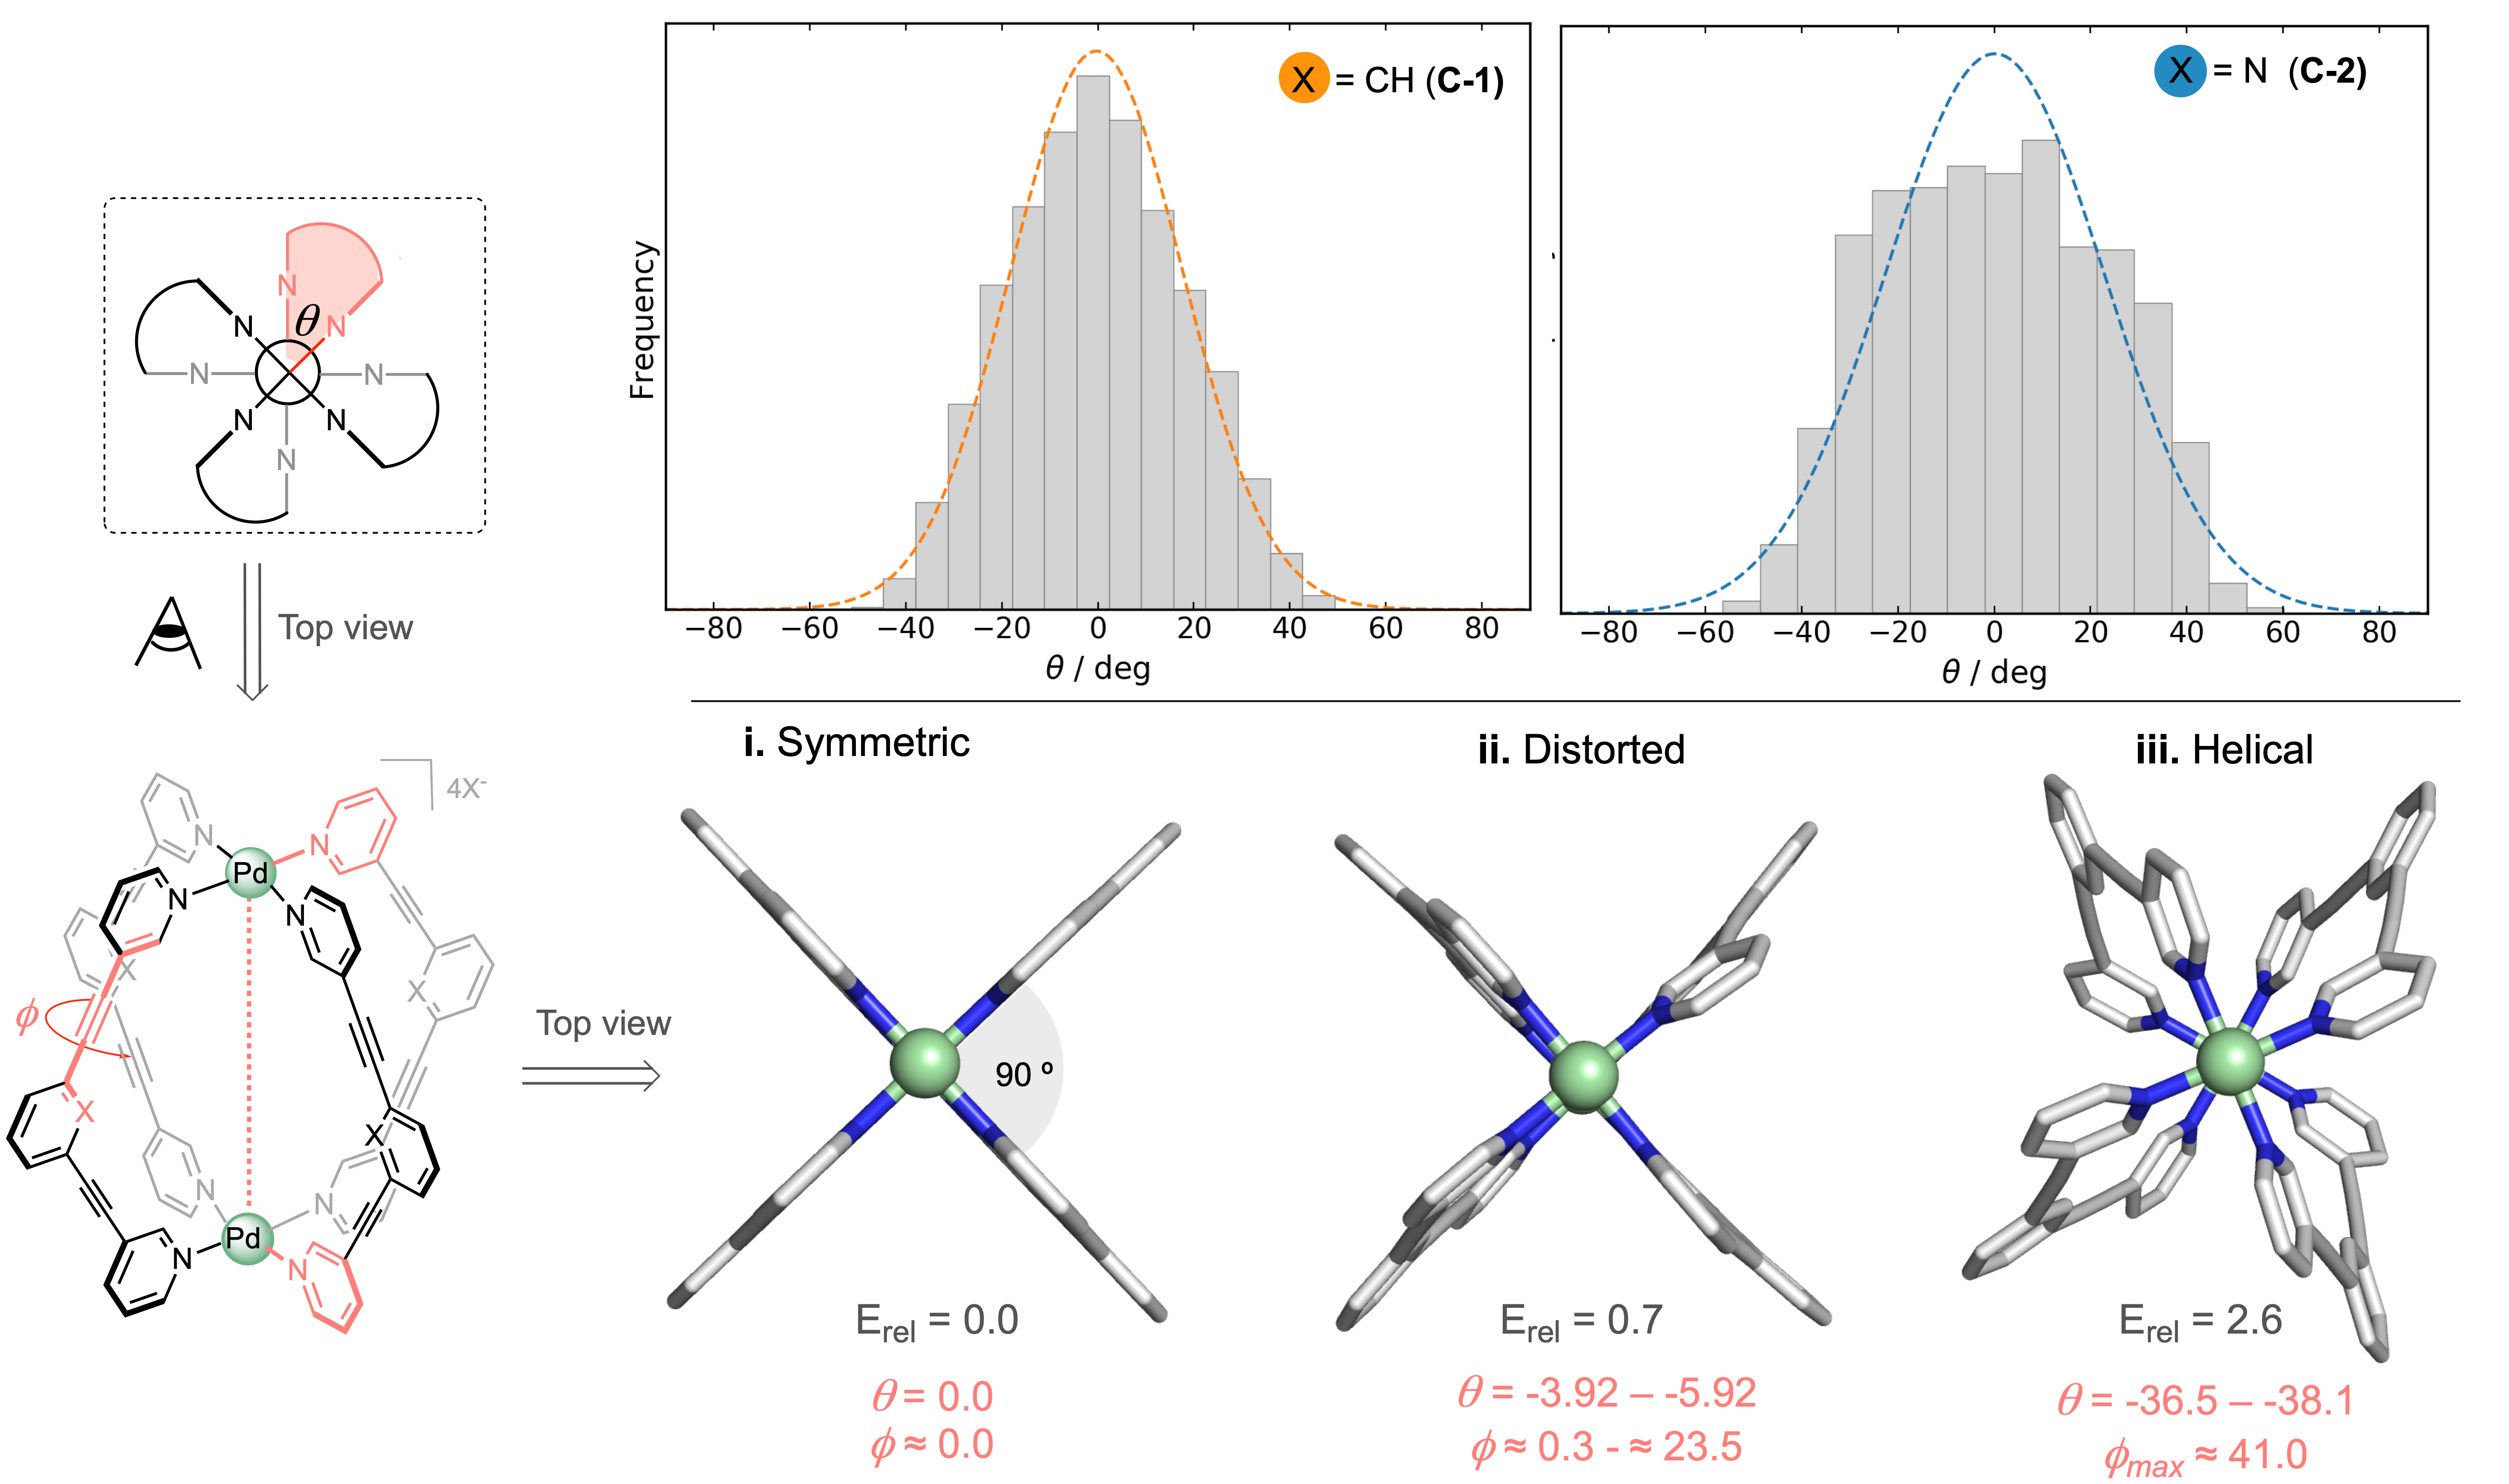
\includegraphics[width=\textwidth]{3/da/figs/fig2/fig2}
	\vspace{0.2cm}
	\hrule
	\caption{(a) Twist angle ($\theta$) frequency for C-1 and C-2 calculated in explicit DCM solvent, over 30 ns of cumulative MD simulations and (b) local minima for C-1 (i-iii) calculated at the PBE0-D3BJ/def2-SVP level of theory. Relative energies ($E_\text{rel}$) in \kcal.}
	\label{fig::da_2}
\end{figure}

\subsubsection{Efficient Protocol for Binding Affinity Calculations}

To quantitatively rationalize catalysis and binding for C-1 and C-2, each with $\sim$150-200 atoms, a computationally efficient protocol is required. Here, we targeted a total time less than the corresponding experiments would take ($\sim$1 day). We selected the M06-2X/def2-TZVP (M2) level of theory, which has been shown to provide accurate association energies for large supramolecular systems.\cite{Sure2015} Furthermore, to compare the binding affinity across a range of quinone/Pd${}_2$L${}_4$ cages, and considering the challenges associated with entropy calculations,\cite{Bootsma2019, Grimme2012, Caldararu2016} we analysed relative potential energy differences ($\Delta\Delta E_\text{bind}$) rather than Gibbs free energy differences ($\Delta\Delta G_\text{bind}$), i.e without considering entropic or zero-point-energy corrections, which cancel when comparing both cages (see detailed discussion in SI).

The binding energy of a general quinone (qn) is defined as $\Delta E_\text{bind}$(qn$\subset$C-X) = $E$(qn$\subset$C-X) – $E$(qn) – $E$(C-X), with negative values suggesting favourable binding; the relative binding affinity between the two cages is then defined as $\Delta\Delta E_\text{bind}$(qn) = $\Delta E_\text{bind}$(qn$\subset$C-2) – $\Delta E_\text{bind}$(qn$\subset$C-1), where positive values indicate a preference of the guest to bind within C-1 over C-2. From Figure \ref{fig::da_3}a and Table \ref{table::si_da_3}, it can be observed that for benzoquinone (bq), in the gas phase, binding is preferred in C-2 over C-1 ($\Delta\Delta E_\text{bind} = -4.5$ \kcal), in contrast to the solution-phase experimental observation. The gas-phase C-2 preference arises from the H-bond interactions between the nitrogen lone pairs ($n$) and the anti-bonding $\sigma$*(C–H) orbitals in bq, which are stronger than the interaction between the C-H group of the meta-substituted benzene and the $\pi$ bond in bq (see below). However, when implicit DCM solvent is introduced, these interactions are almost entirely masked, leading to a preference for C-1 over C-2, in agreement to experimental results (calcd. $\Delta\Delta E_\text{bind}$ = +1.9 \kcalx cf. expt.\cite{MartCentelles2018} $\Delta\Delta G_\text{bind}$ = +1.2 \kcal). For the larger guest anthraquinone (aq), for which the $n \rightarrow \sigma$*(C–H) interactions are not possible, binding in C-1 is favoured in both gas and solvent phase, in good agreement with experiment (calcd. $\Delta\Delta E_\text{bind}$= +3.7 \kcalx cf. expt. $\Delta\Delta G_\text{bind}$= +5.1 \kcal). Pleasingly, the absolute binding affinity of bq was also predicted to within chemical accuracy (Figure \ref{fig::da_3}), which suggest that entropic corrections to the free energy of binding are negligible for this system i.e. calcd. $\Delta E_\text{bind} \approx$ expt. $\Delta G_\text{bind}$. (see detailed discussion in SI §\ref{section::da_si_3_3}).\footnote{$G_\text{bind} = E_\text{bind}+\text{ZPE} + E_\text{therm}+P\Delta V–T \Delta S$. The last three terms are obtained from frequency calculations assuming an ideal gas model (IGM)} 

\begin{figure}[h!]
	\vspace{0.4cm}
	\centering
	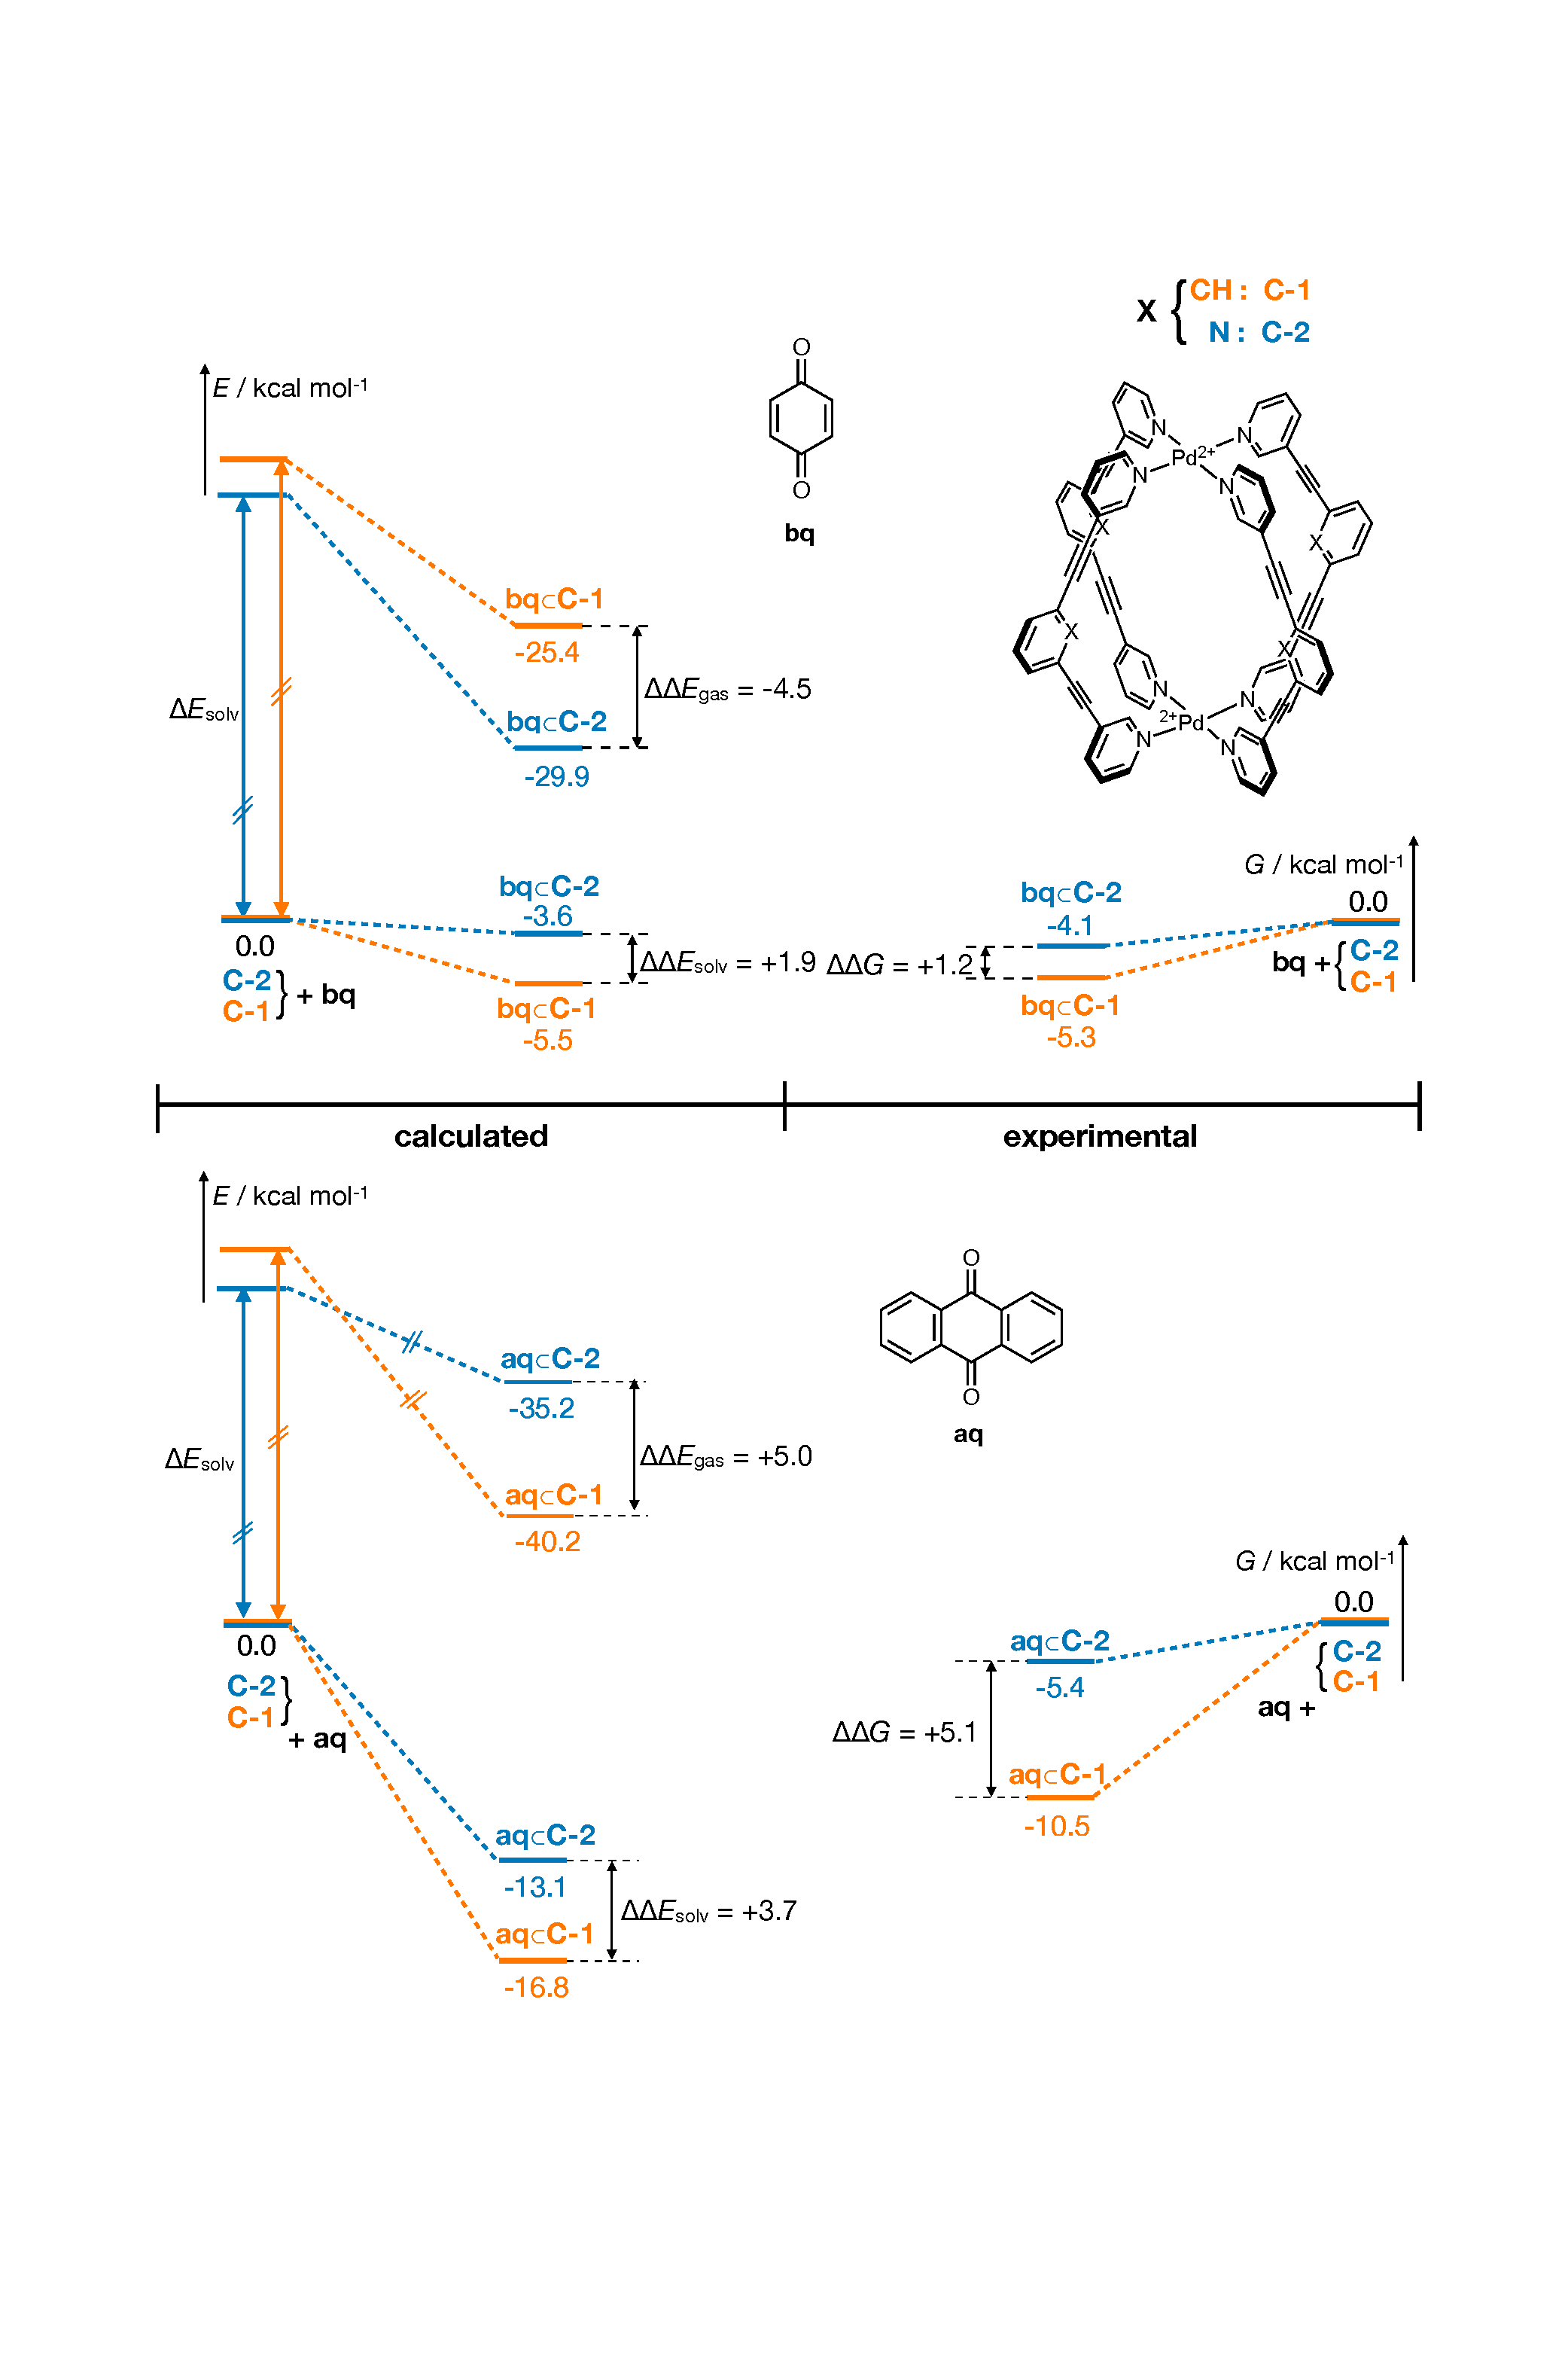
\includegraphics[width=13.5cm]{3/da/figs/fig3/fig3.pdf}
	\vspace{0.2cm}
	\hrule
	\caption{Calculated and experimental absolute and relative binding affinities for (a) bq$\subset$C-1 and bq$\subset$C-2. Experimental values were obtained in dichloromethane (DCM) solvent at room temperature. Gas phase and solution phase calculations performed at the M06-2X/def2-TZVP and SMD(DCM)-M06-2X/def2-TZVP level of theory, respectively. Values reported in Table \ref{table::si_da_3}.}
	\label{fig::da_3}
\end{figure}

The absolute binding affinities of aq are overestimated ($\Delta E_\text{bind}= -16.8 (-13.1)$ vs $\Delta G_\text{bind} = -10.5 (-5.4)$ \kcalx for C-1(C-2), Table \ref{table::si_da_3}), potentially arising from the significant loss in rotational entropy of aq compared to bq upon binding, in which case $\Delta S$ is no longer negligible. Nevertheless, the relative binding energies for both cages compare well to experiment. These results demonstrate that the predicted relative binding affinities for bq and aq between C-1 and C-2 are accurate to within $\sim$2 \kcal. To probe whether this result was general for this class of system, we considered 14 experimental binding affinities (guest molecules shown in Figure \ref{fig::si_da_15}) for C-1 and C-2, including a new data point corresponding to pentacenedione (q4) bound to C-2. Bearing in mind the computational expense of performing geometry optimizations for this set at the SMD(DCM)-M2 level of theory (five days on a CPU with 8 cores), calculations were performed at the more efficient M1 level, followed by single point energy evaluations at SMD(DCM)-M2. We refer to this approach as SMD(DCM)-M2//M1 (Table \ref{table::si_da_8}).

In these systems, both relative ($\Delta\Delta E_\text{bind}$) and absolute binding energies ($\Delta E_\text{bind}$) were calculated (Figure \ref{fig::da_4}). Once again, not only are the relative binding affinities obtained to within a reasonable mean absolute deviation (MAD = 2.2 \kcal), the absolute binding affinities are close to chemical accuracy (MAD = 1.7 \kcal, Figure \ref{fig::da_4}, Table \ref{table::si_da_8}), with calculations taking less than a day on a CPU with 8 cores. Compared to predictions in organic host-guest complexes, e.g. via the Statistical Assessment of the Modelling of Proteins and Ligands (SAMPL) challenge, where errors of at least 1–4 \kcalx and correlations ($r^2$) below 0.5 have been reported, our correlation to experimental binding affinities ($r^2$ = 0.759) can be considered very good.\cite{Sure2015, Jensen2015, Rizzi2018}
 
The binding affinity outlier is tert-butyl benzoquinone (top right in Figure \ref{fig::da_4}a), for which we find binding within the cavity to be unfavourable. Experimentally, this quinone has been hypothesized to bind to the outer ‘pocket’ of the cage, i.e. expt. $\Delta G_\text{bind}$ of encapsulation may, in fact, be positive. We also hoped to further accelerate the methodology by obtaining structures at a semi-empirical (PM7\cite{Stewart2012}) or tight-binding DFT (GFN-xTB\cite{Grimme2017xtb}) level of theory. Unfortunately, these methods lead to relatively poor correlation ($r^2$(SMD(DCM)-M2//PM7) = 0.309, $r^2$(SMD(DCM)-M2//GFN-xTB) = 0.173, Figures \ref{fig::si_da_9}--\ref{fig::si_da_11}). Note the latter is in spite of the relatively small root mean squared deviation (RMSD) to M1 geometries ($0.3\pm0.2$ \AA). 

\begin{figure}[h!]
	\vspace{0.4cm}
	\centering
	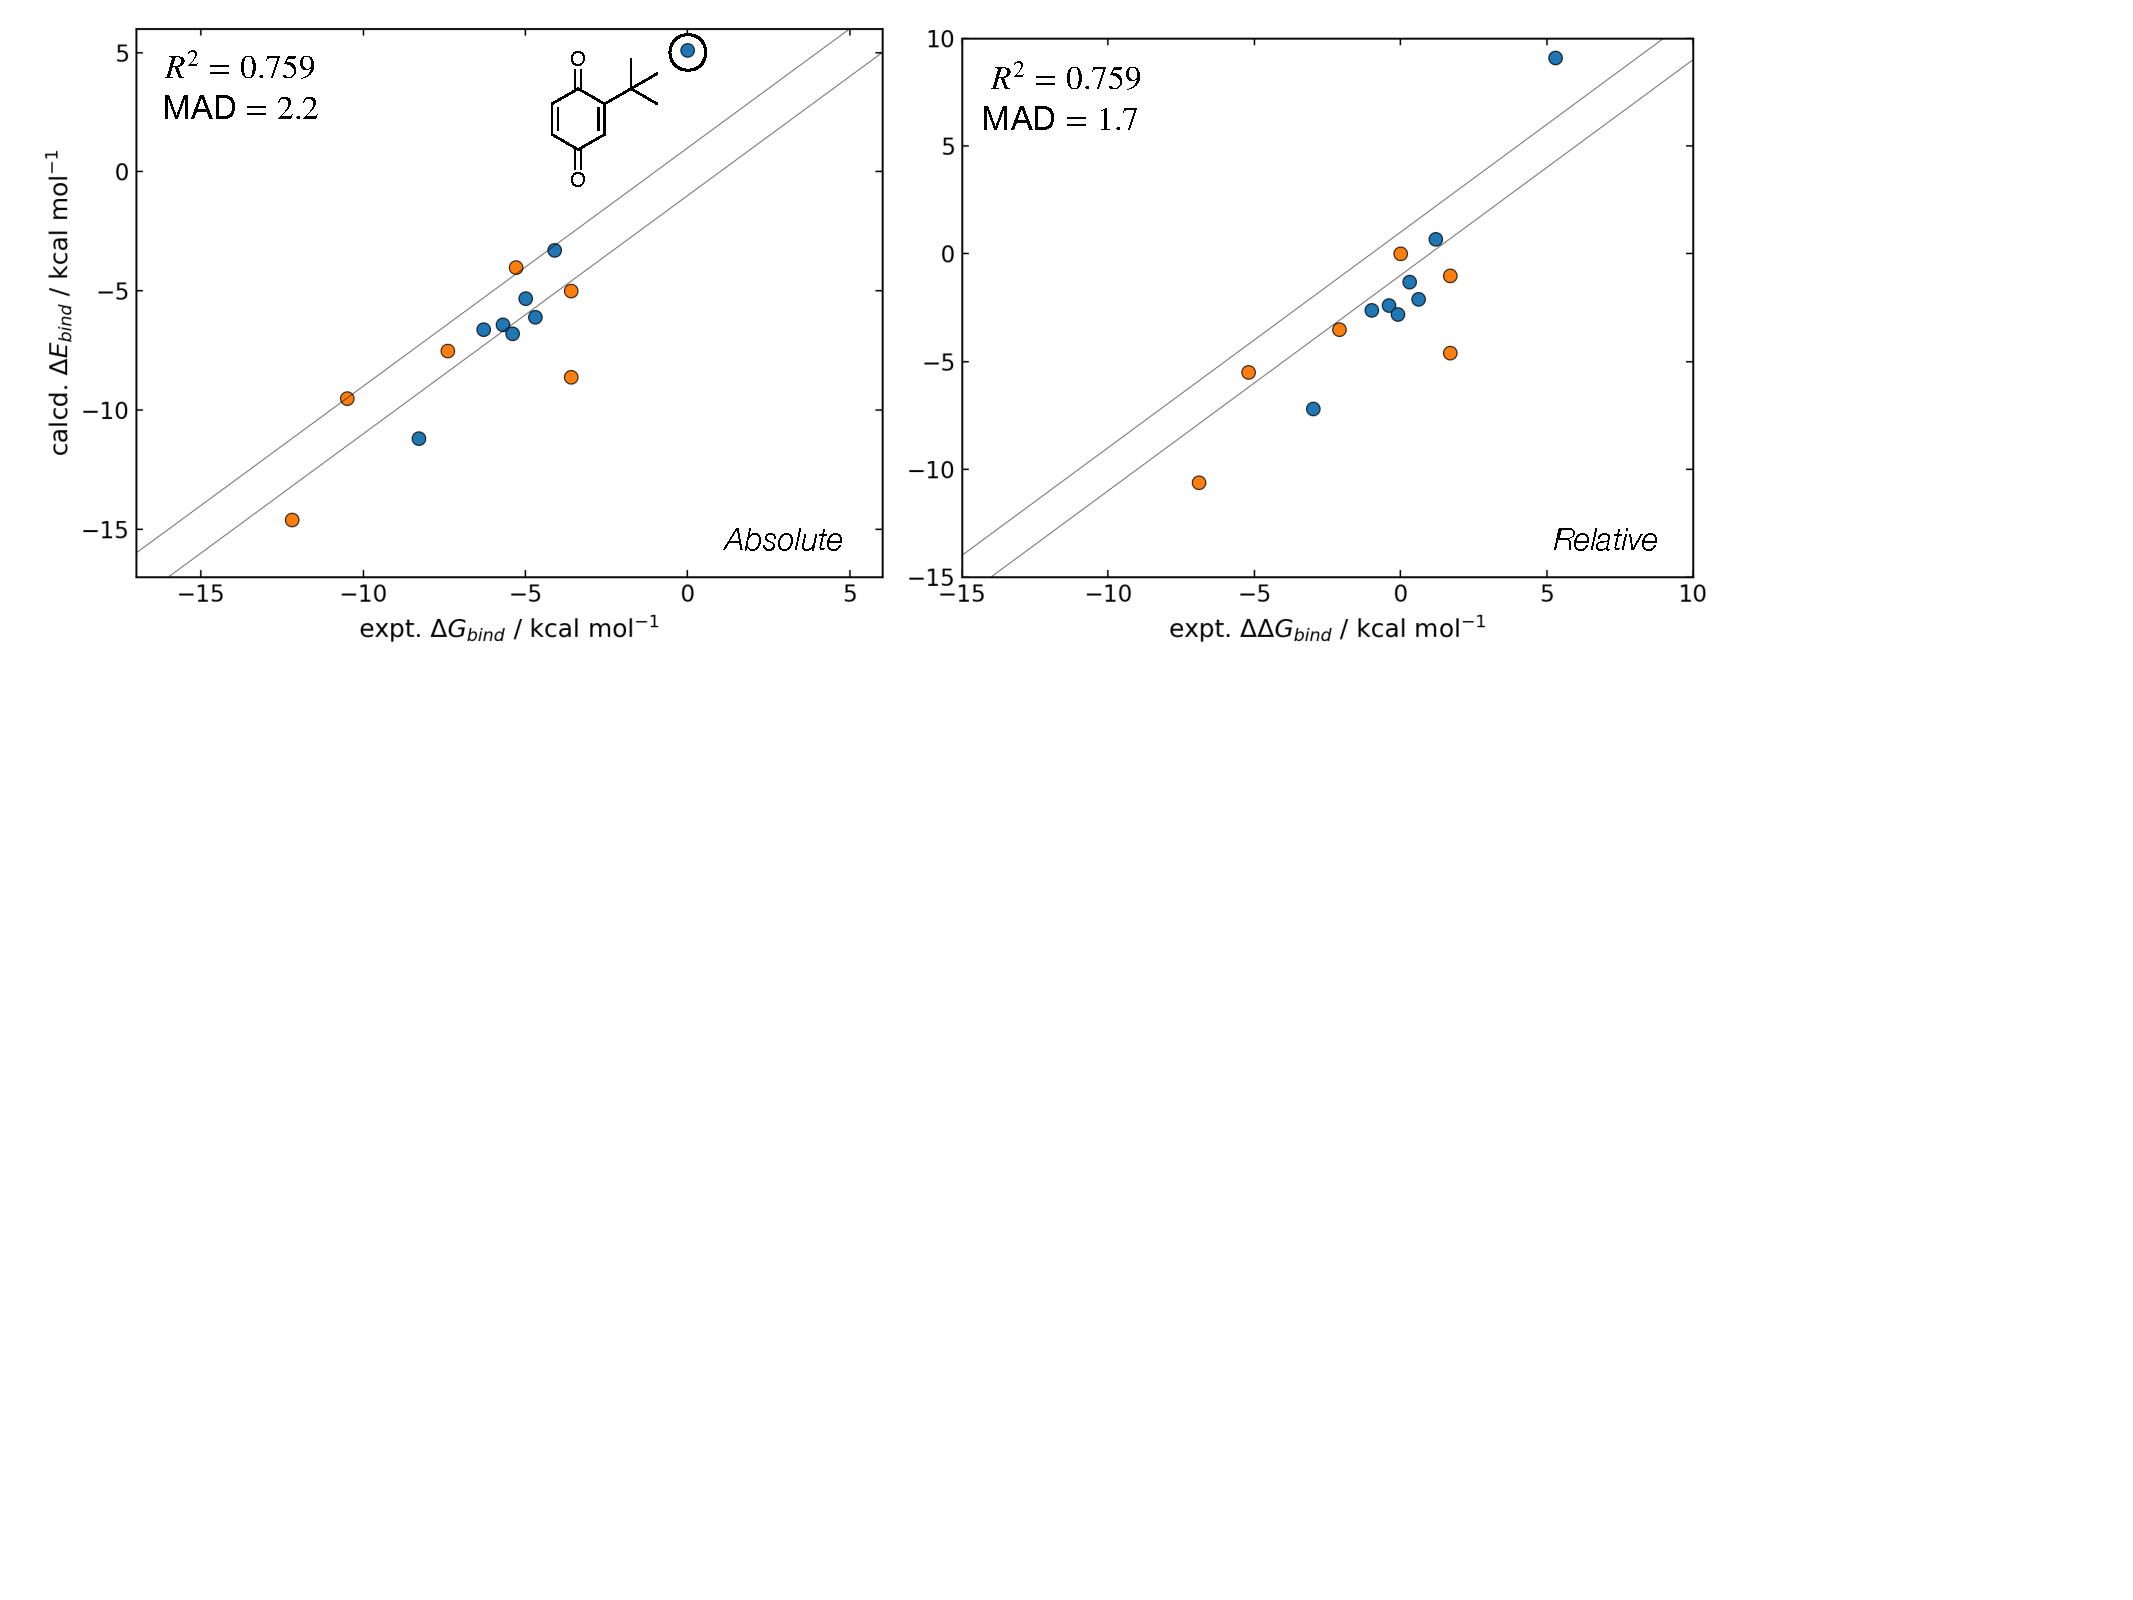
\includegraphics[width=\textwidth]{3/da/figs/fig4/fig4.pdf}
	\vspace{0.2cm}
	\hrule
	\caption{Correlation plots of (a) $\Delta\Delta E_\text{bind}$ = $\Delta E_\text{bind}$(qn$\subset$C-X) – $\Delta E_\text{bind}$(bq$\subset$C-1). and (b) $\Delta E_\text{bind}$ calculated at the SMD(DCM)-M06-2X/def2-TZVP//PBE0-D3BJ/def2-SVP level of theory to experimental free energies. Orange and blue markers corre-spond to C-1 and C-2 cages, respectively. The different diagonals bracket the ±1 \kcalx area of accuracy. The dash line represents the line of best fit.}
	\label{fig::da_4}
\end{figure}


\subsubsection{Rationalizing Differences in Binding Affinities}
 To elucidate the nature of the non-covalent interactions driving quinone binding, and the differences between C-1 and C-2, we constructed two reduced models. The first uses\\ [Pd(pyridine)$_4$]$^{2+}$ as a model of the “top” and “bottom” of the cage (model 1, Figure \ref{fig::da_5}a), while the second describes the interaction between the quinone guest with the central meta-substituted benzene or 2,6-pyridyl groups in C-1 and C-2, respectively (model 2, Figure \ref{fig::da_5}b). 

Using model 1 we analyse the effect of the metal and the +2 charge it introduces Figure \ref{fig::da_5}a, by comparing the canonical complex ([Pd(pyridine)$_4$]$^{2+}$,  light blue) to a complex without metal and an overall +2 charge ([(pyridine)$_4$]$^{2+}$, cyan), and without metal and an overall zero charge ([(pyridine)$_4$], green). This model demonstrates that the metal influences binding by mainly introducing a positive charge that polarizes the adjacent \emph{o}-pyridine (C)H donor groups (Figure \ref{fig::da_5}a and \ref{fig::si_da_16}). The second model, model 2, describes the interaction between the quinone guest with the `equatorial' meta-substituted phenyl or pyridyl moieties. In this system, rotation of bq around the z-axis (defined by the angle $\chi$, Figure \ref{fig::da_5}b-c) shows a minimum at $\chi \approx$ 0${}^\circ$ for the bq$\subset$[(pyridine)${}_4$] system (blue line), while for the bq$\subset$[(benzene)${}_4$] system (orange line), minima are found at $\chi \pm 45{}^\circ$. In the former, electron donation from the nitrogen lone pair ($n$) to the anti-bonding $\sigma$*(C–H) orbital leads to the formation of weak hydrogen bonds at $\chi = 0^\circ$ (Figure \ref{fig::si_da_17}, \ref{fig::si_da_18}).\cite{Lewis2013} In contrast, for the bq$\subset$[(benzene)$_4$] system, repulsion between CH groups produces a maximum at the same position (Figure \ref{fig::da_5}b). This explains why in C-1, bq sits out of the plane of opposing ligands in ($\chi \approx$ 45${}^\circ$), while in C-2, bq lies in the plane ($\chi \approx$ 0${}^\circ$, Figure \ref{fig::da_5}c). The $n \rightarrow \sigma$*(C–H) interactions are strong in the gas phase; however, due to their electrostatic nature, they are lost once implicit solvent is included. In contrast, while the $\pi \rightarrow \sigma$*(C–H) interactions are relatively weak, they are less dependent on the solvent and contribute to the binding of the guest within C-1 (Figure \ref{fig::si_da_19}). These results explain the observed preference for binding qn within C-1 over C-2, which originates from differences in solvation energy, with C-2 being the intrinsically stronger binder. 

\begin{figure}[h!]
	\vspace{0.4cm}
	\centering
	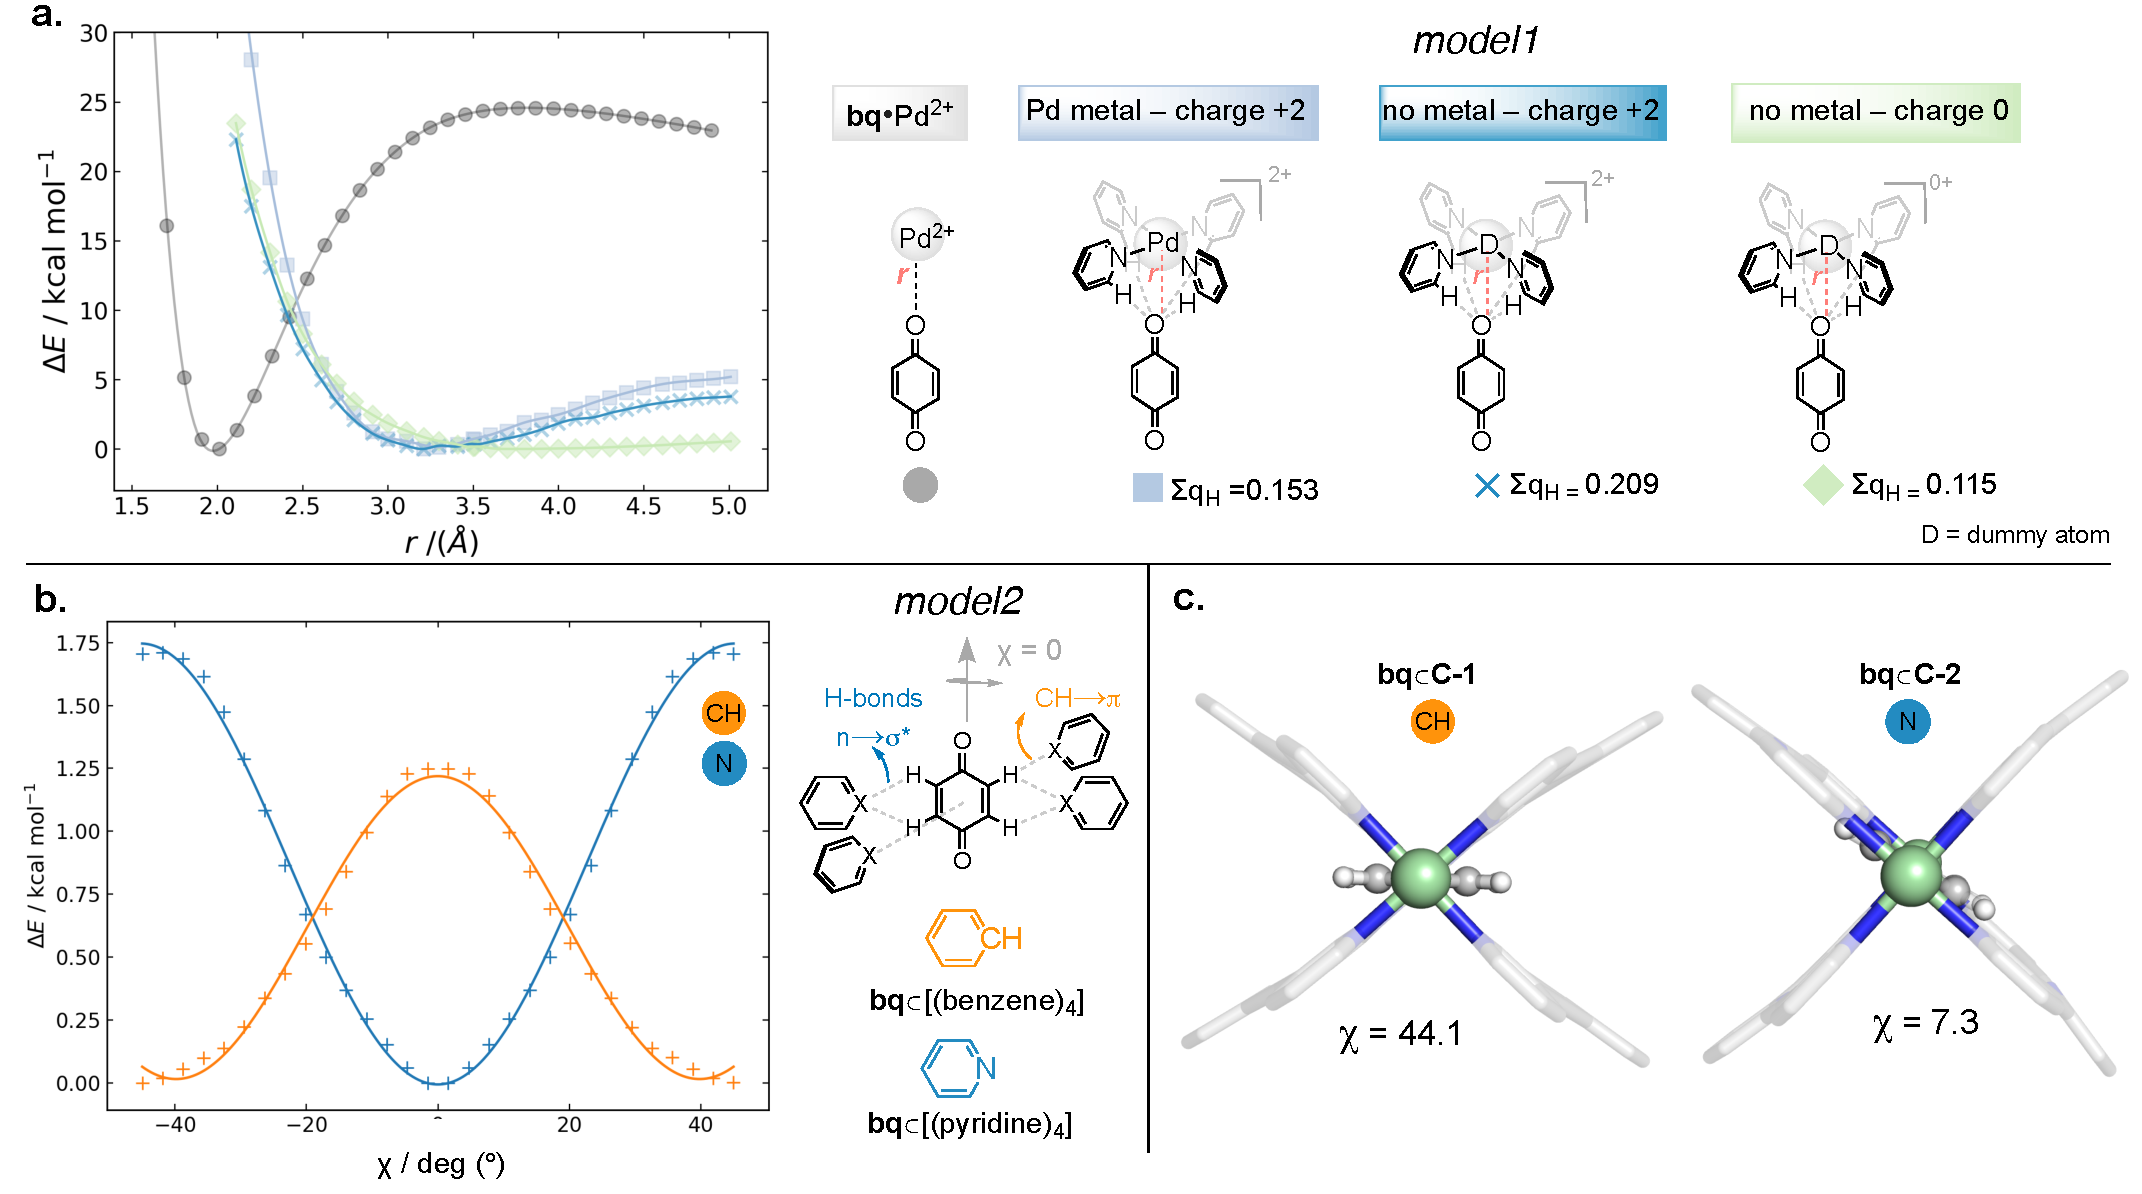
\includegraphics[width=\textwidth]{3/da/figs/fig5/fig5.pdf}
	\vspace{0.2cm}
	\hrule
	\caption{(a) Comparative PES for bq with Pd(II) (grey), the canonical complex ([Pd(pyridine)$_4$]$^{2+}$, light blue) complex without metal and an overall +2 charge ([(pyridine$_4$]$^{2+}$, cyan), and complex without metal and an overall zero charge ([(pyridine)$_4$]$^0$, green). The sum of atomic partial charges on the (C)H atoms, using the Hirshfeld scheme, is shown in each case (b) Non-covalent interaction in model 2, including benzenes/pyridines and bq. (c) Global minima of bq$\subset$C-1 and bq$\subset$C-2. All calculated at the M06-2X/def2-TZVP level of theory.}
	\label{fig::da_5}
\end{figure}

\subsubsection{Rationalizing the Differences in Catalytic Activity}
	
To assess the influence of the cages on DA reactivity, the activation energies for a set of 10 uncatalysed reactions (Figure \ref{fig::si_da_20}) were calculated using a highly accurate quantum chemical method. Pleasingly, the error to experiments\cite{MartCentelles2018} was within $\pm$1 \kcalx (MAD = 0.9 \kcalx). Among the different DFT functionals tested, the M2 method was found to have the lowest error relative to the \emph{ab initio} results (MAD 1.2 \kcalx for reaction barriers and 1.7 \kcalx for reaction energies, Figures \ref{fig::si_da_21}, \ref{fig::si_da_22}). In all cases, a highly synchronous transition state (TS) was observed, with the endo cycloadduct being preferred (Table \ref{table::si_da_11_12}). These results are in agreement with previous computational studies on the uncatalysed reaction of para-quinone imine derivatives using the M06-2X functional in vacuum.\cite{Uliana2014}

With a chemically accurate computational methodology in hand, the reaction barriers for the DA reaction between bq and isoprene (d1) in the presence of C-1 or C-2 were calculated. Formation of an association complex between d1 and bq$\subset$C-1/C-2 is unfavourable. For example, with C-2 it leads to a complex 8.8 \kcalx higher in free energy than bq$\subset$C-2 and isoprene separately (Table \ref{table::si_da_16}). This result is in line with ${}^1$H NMR data of the catalytic process, which shows that neither the cage nor the quinone signals shift upon addition of diene to the reaction,\cite{MartCentelles2018} and contrast with most supramolecular host-guest complexes exhibiting DA catalytic activity, where a so-called “ternary Michaelis complex” is observed.\cite{Daver2017} As suggested experimentally, our calculations confirm that the complex bq$\subset$C-2 is first formed and then reacts intermolecularly with an incoming isoprene molecule. 

Defining the catalytic activity as $\Delta\Delta E_\text{CA}$ = $\Delta E_\text{uncat}^\ddagger$ - $\Delta E_\text{cat}^\ddagger$ , such that positive values correspond to effective catalysis we calculate $\Delta\Delta E_\text{CA}$ (d1+bq$\subset$C-2) = $+5.4$ \kcalx (expt. $\Delta\Delta G_\text{CA}$  = +3.6 \kcalx) while $\Delta\Delta E_\text{CA}$ (d1+bq$\subset$C-1) = $-0.3$ \kcalx (expt. catalytically inactive, Table \ref{table::da1}). As shown in Figure \ref{fig::da_6}a, while C-1 binds the substrate more strongly in the reactant state, C-2 provides a better stabilisation at the TS and slightly better stabilization of the product state (Figure \ref{fig::si_da_25}). Analysis of the encapsulated TS geometries indicate that, for asymmetric dienes, the cage increases the asymmetric nature of the TSs compared to the uncatalysed analogues, making it less pericyclic and more stepwise (Figure \ref{fig::da_6}b). The active C-2 cage affords a slightly more asynchronous reaction ($\Delta d$ = 0.28/$-0.17$, 0.36/$-0.23$ \AA$\;$ for TS[d1+bq$\subset$C-1] and TS[d1+bq$\subset$C-2], respectively). 
To rationalize these differences, we explored the electronic and steric contributions to the reaction energy in each system. In both cases, and as previously seen for Lewis acid-catalysed [4+2] cycloadditions,\cite{Fringuelli2002, Corey2002, Liu2015} the cages enhance the electrophilic character of the dienophile bound in the cavity. Polarization of the dienophile within the cage leads to a net charge of +0.25 and +0.16 in bq for C-1 and C-2, respectively,\cite{MartCentellesDuarte2018} leading to a lowering the LUMO energy by 1.5 and 1.6 eV in C-1 and C-2, respectively (see full SI). These results, demonstrate that both C-1 and C-2 can activate the dienophile by reducing its LUMO energy. However, as discussed below, other interactions in C-1 offset this activating effect. To analyse this contrasting behaviour between C-1 and C-2, we performed an energy decomposition analysis using the distortion/interaction framework.\cite{Ess2007} Within this framework, the activation energy of a reaction ($\Delta E^\ddagger$) is partitioned into the energy required to distort the reactants from their ground-state to their transition state geometry ($\Delta E^\ddagger_\text{dist}$) and the energy of interaction between these fragments ($\Delta E^\ddagger_\text{int}$). For the reaction under study, the optimal interaction between the activated dienophile and the incoming diene takes place within one of the cage portals (Figure \ref{fig::da_6}b); this requires the ligand to distort significantly, thus suggesting that distortion of the cage and the substrate is required to reach the TS in the cage-catalysed process.

\begin{figure}[h!]
	\vspace{0.4cm}
	\centering
	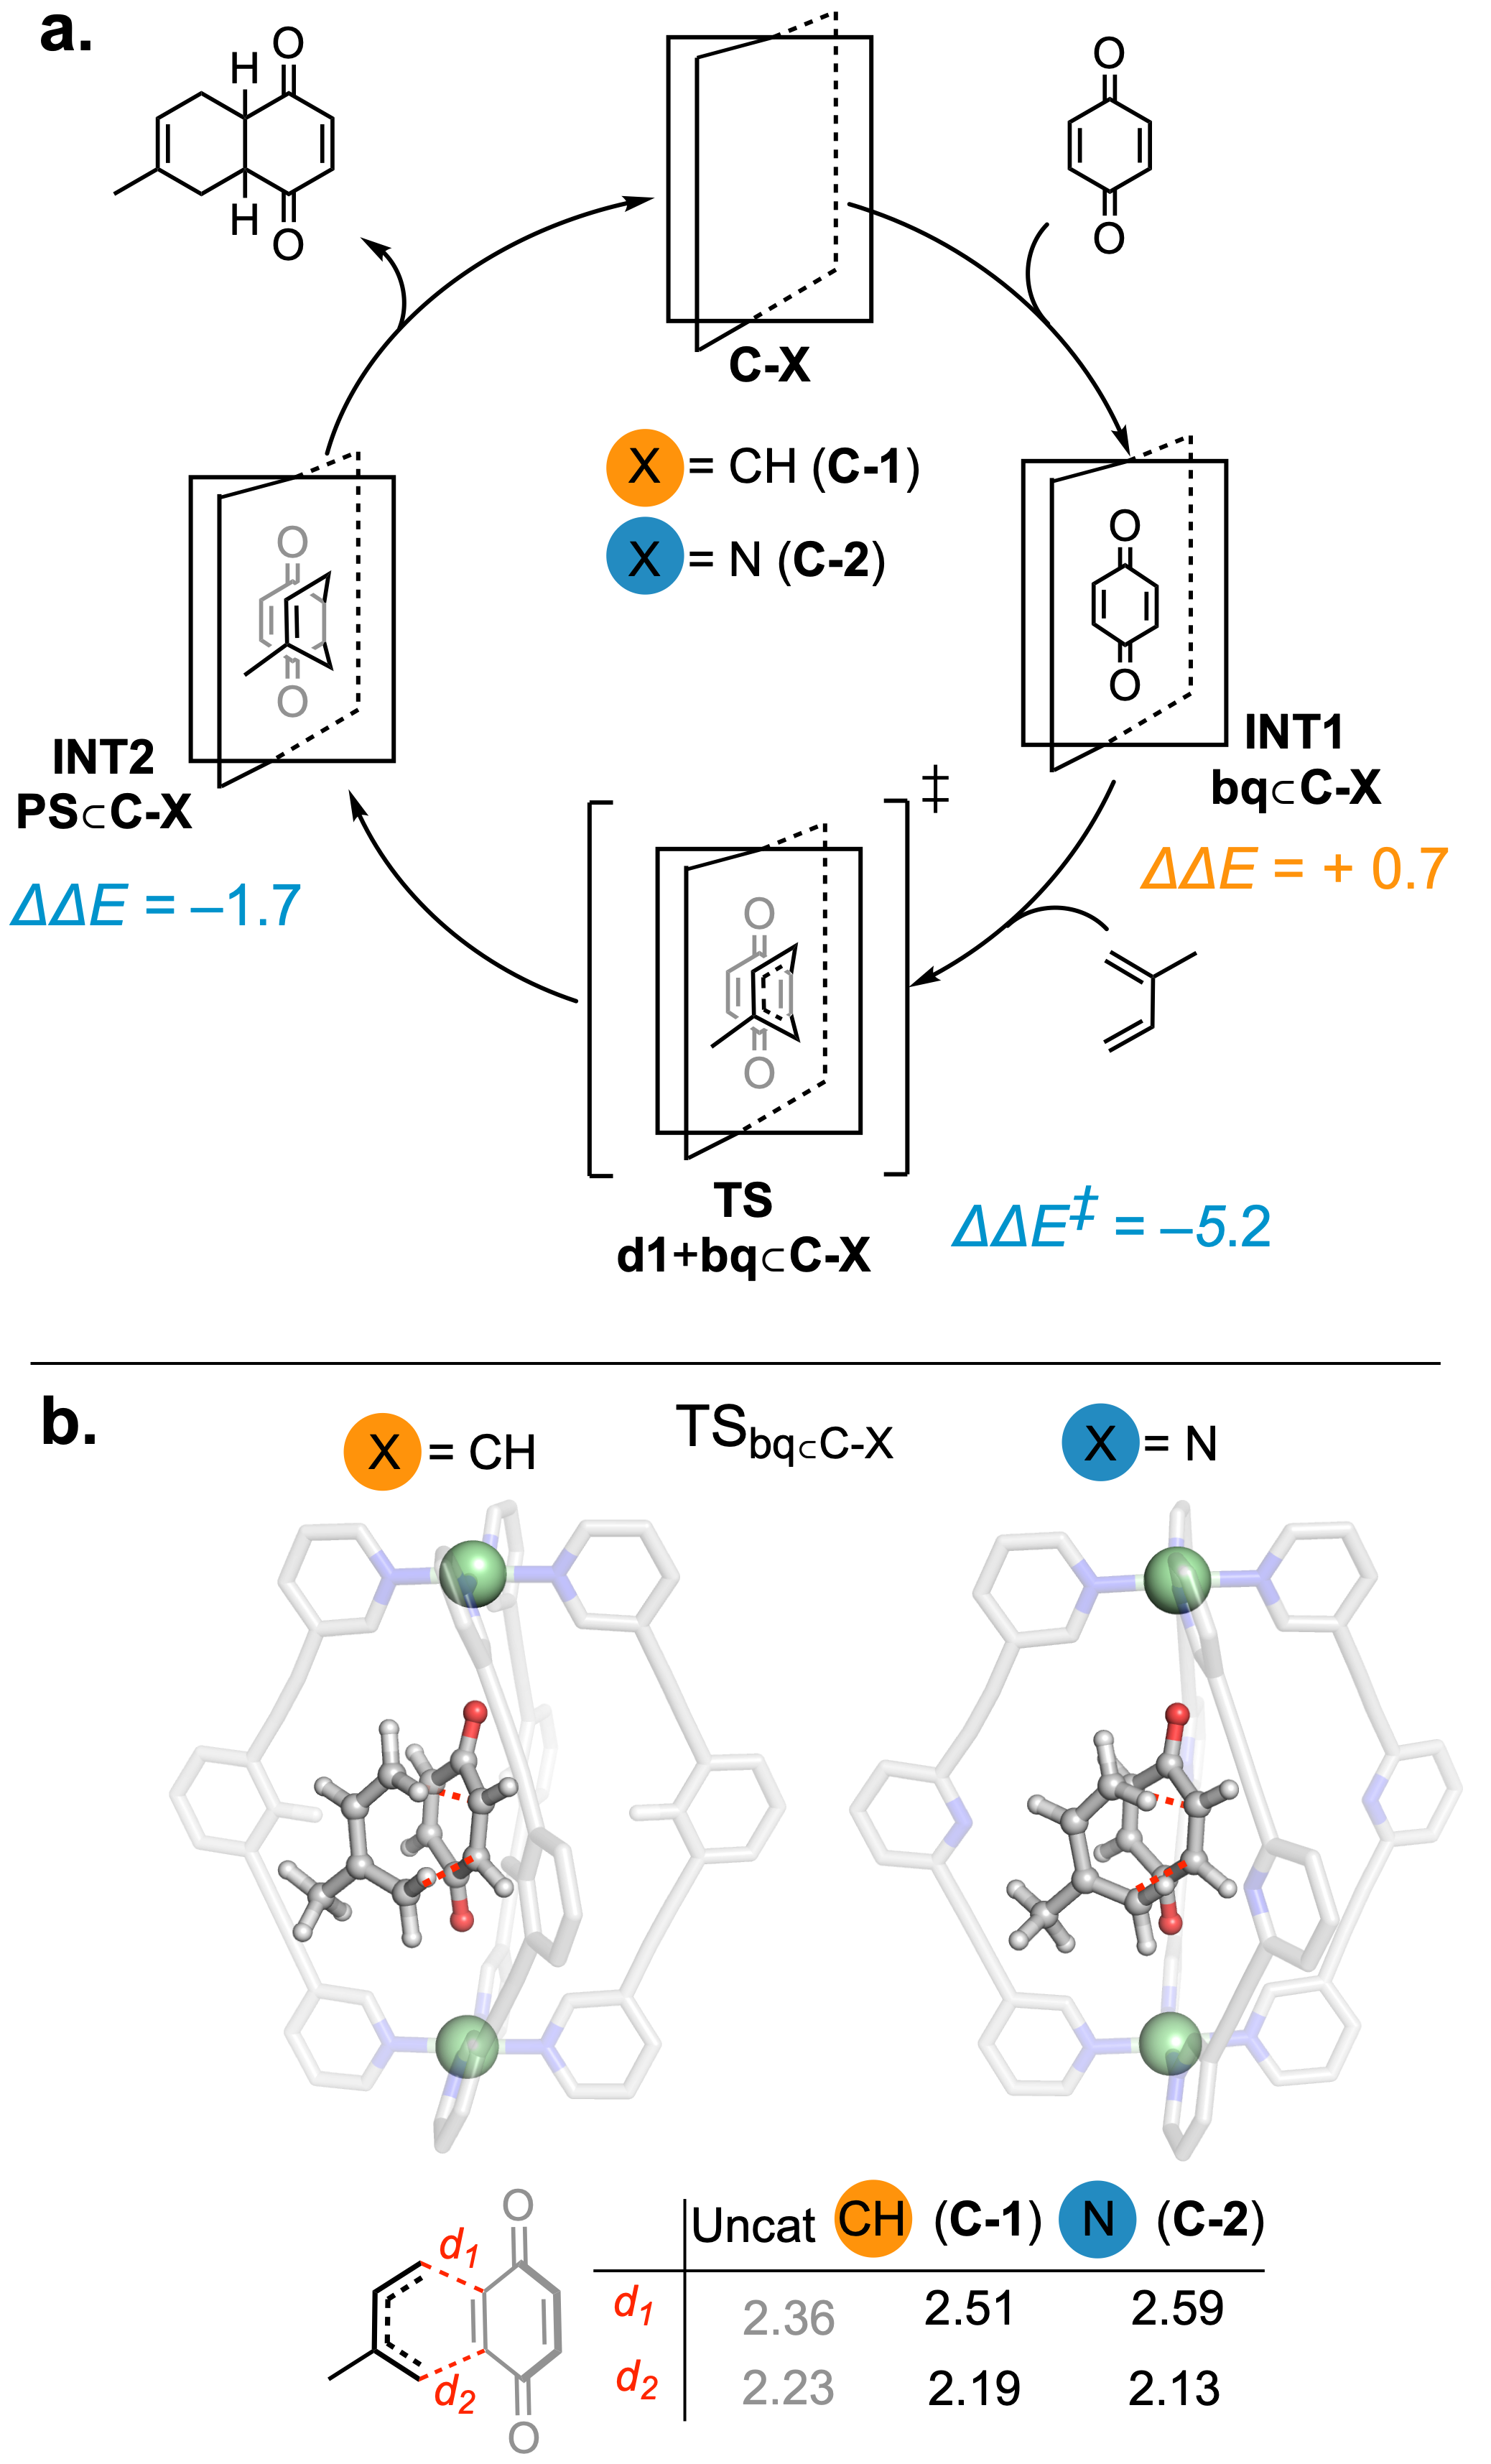
\includegraphics[width=8.5cm]{3/da/figs/fig6/fig6}
	\vspace{0.2cm}
	\hrule
	\caption{(a) Catalytic cycle for the reaction between benzoquinone and isoprene ($\Delta\Delta E$ = $\Delta E$(C-2) – $\Delta E$(C-1) in \kcalx at SMD(DCM)-M06-2X/def2-TZVP//PBE0-D3BJ/def2-SVP, negative(positive) values in blue(orange) refer to favourable stabilization for C-2 (C-1)). (b) Optimized TS geometries; Distances (\AA) of the forming bonds at the TS for the uncatalysed (grey) and encapsulated (black) reaction.}
	\label{fig::da_6}
\end{figure}


\begin{table}[h!]
	\def\arraystretch{2.0}
	\begin{tabularx}{\textwidth}{YYYYYYYY}
		\hline
		& \small{$\Delta E^\ddagger_d$ [C-X]} &\small{$\Delta E^\ddagger_d$ [diene]}&	\small{$\Delta E^\ddagger_d$ [bq]}&	\small{$\Delta E^\ddagger_d$ [bq$\subset$C-X]} &	\small{$\Delta E^\ddagger_d$[bq$\subset$C-X +diene]} &  \small{$\Delta E^\ddagger_\text{int}$} & \small{$\Delta E^\ddagger$
}\\
		\hline
		Uncat.         	&--	 &   15.8 	&7.1	&--	&22.9${}^a$&	-13.0&	9.9
\\
		C-1	               &5.2	  &  16.2&	8.8	  &13.2&	29.4&	-19.2&	10.2
\\
		C-2               &	5.1	 &   14.9	&9.3&	10.0&	24.9&	-20.4&	4.5
\\
		$\Delta\Delta E_\text{C2-C1}$ &	-0.1	&-1.3&	0.5	&-3.2&	-4.5&	-1.2&	-5.7
\\
	\end{tabularx}
\hrule
\caption{Distortion/Interaction Analysis for the [4+2] cyclisation of isoprene with benzoquinone calculated at the SMD(DCM)-M2 level of theory. Shown here are the distortion energies of the cage ($\Delta E^\ddagger_d$[cage]), substrate ($\Delta E^\ddagger_d$[diene]), dienophile ($\Delta E^\ddagger_d$[bq]), and bq$\subset$C-X complex ($\Delta E^\ddagger_d$[bq$\subset$C-X]). The interaction energy is defined as $\Delta E^\ddagger_\text{int}$ = $\Delta E^\ddagger - \Delta E^\ddagger_d$, where $\Delta E^\ddagger$ is the activation energies and total $\Delta E^\ddagger_d$ = $\Delta E^\ddagger_d$[bq$\subset$C-X] + $\Delta E^\ddagger_d$[diene]. All energies are given in \kcal. $a.$ Sum of diene and quinone distortion.}
\label{table::da1}
\end{table}

The energetic cost of distorting each component of the reaction is shown in Table 1. Here, we separated each TS structure into three fragments ($\Delta E_d^\ddagger$[C-X], $\Delta E_d^\ddagger$[diene], and $\Delta E_d^\ddagger$[bq]) and also evaluated the bq$\subset$C-X complex as a single fragment ($\Delta E_d^\ddagger$[bq$\subset$C X]). In C-2 a smaller distortion compared to C-1 is obtained for both the diene (1.3 \kcal) and the cage-dienophile complex (4.5 \kcal). For C-1, the cost of aligning the dienophile bq with the cage portal is found to be twice the cost seen in C-2 (Figure \ref{fig::si_da_29}). This can be associated to steric clashes arising between the central moiety of L${}^\text{CH}$ and the dienophile. This effect can be visually understood through the use of non-covalent interaction (NCI) plots, which in C-1 shows steric clashes between the dienophile and the cage, while in C-2 these regions are smaller and compensated by a favourable N$\cdots$HC hydrogen interaction between the diene and the cage. The latter may also lead to the slightly more positive interaction term for this cage (Figure \ref{fig::si_da_29}). For both cages, the interaction energy ($\Delta E^\ddagger_\text{int}$) is more favourable compared to the uncatalysed reaction, which is in line with lowering of dienophile LUMO energy. However, distortion effects render C-1 uncatalytic. These results demonstrate that small differences in cage sterics and flexibility play an important role in determining the potential catalytic activity of very similar metallocages towards a given reaction. Such energetic costs will vary depending on the activation mode required and the nature of the substrates involved but can be easily quantified. 
Finally, while our analysis in Table \ref{table::da1} included only potential energies, Gibbs free energies can be obtained by adding thermal and entropic contributions (Table \ref{table::si_da_20}). By doing so, we obtain $\Delta G_\text{uncat}^\ddagger$ = 23.5 \kcalx and $\Delta G_\text{cat}^\ddagger$ (C-1/C-2) = 23.6/18.8 \kcal, which are in good agreement with experimental results and confirm that catalysis in C-2 is enthalpic in origin.

\subsubsection{Efficient Protocol for Calculating Catalytic Activity}

Having rationalized the catalytic properties of the two cages for a single cycloaddition reaction, we sought to validate our methods with a wider range of substrates. Although fully optimized TSs for the DA reactions outlined in Figure \ref{fig::da_7} can be located within these cages, the computational demand is significant, even using a low level of theory ($>3$ days on a CPU with 8 cores). With the aim to decrease this time, we proposed to evaluate catalytically promising cages considering the following approximations: (1) To rely on potential energy rather than free energies differences, and (2) to calculate the activation energy of ‘TS analogues’ rather than the true transition state. We use the term ‘TS analogues’ to indicate that the bonds being formed and broken are constrained to the distance values found in the uncatalysed TS. 

The catalytic activity ($\Delta\Delta E'_\text{CA}$) is then found by performing a constrained minimization and comparing to the uncatalysed variant (Figure \ref{fig::da_7}). This computationally inexpensive approach can achieve 80\% accuracy in predicting the catalytic proficiency towards the DA reactions tested (Figure \ref{fig::da_7}), while providing a ten-fold reduction in computational time.


\begin{figure}[h!]
	\vspace{0.4cm}
	\centering
	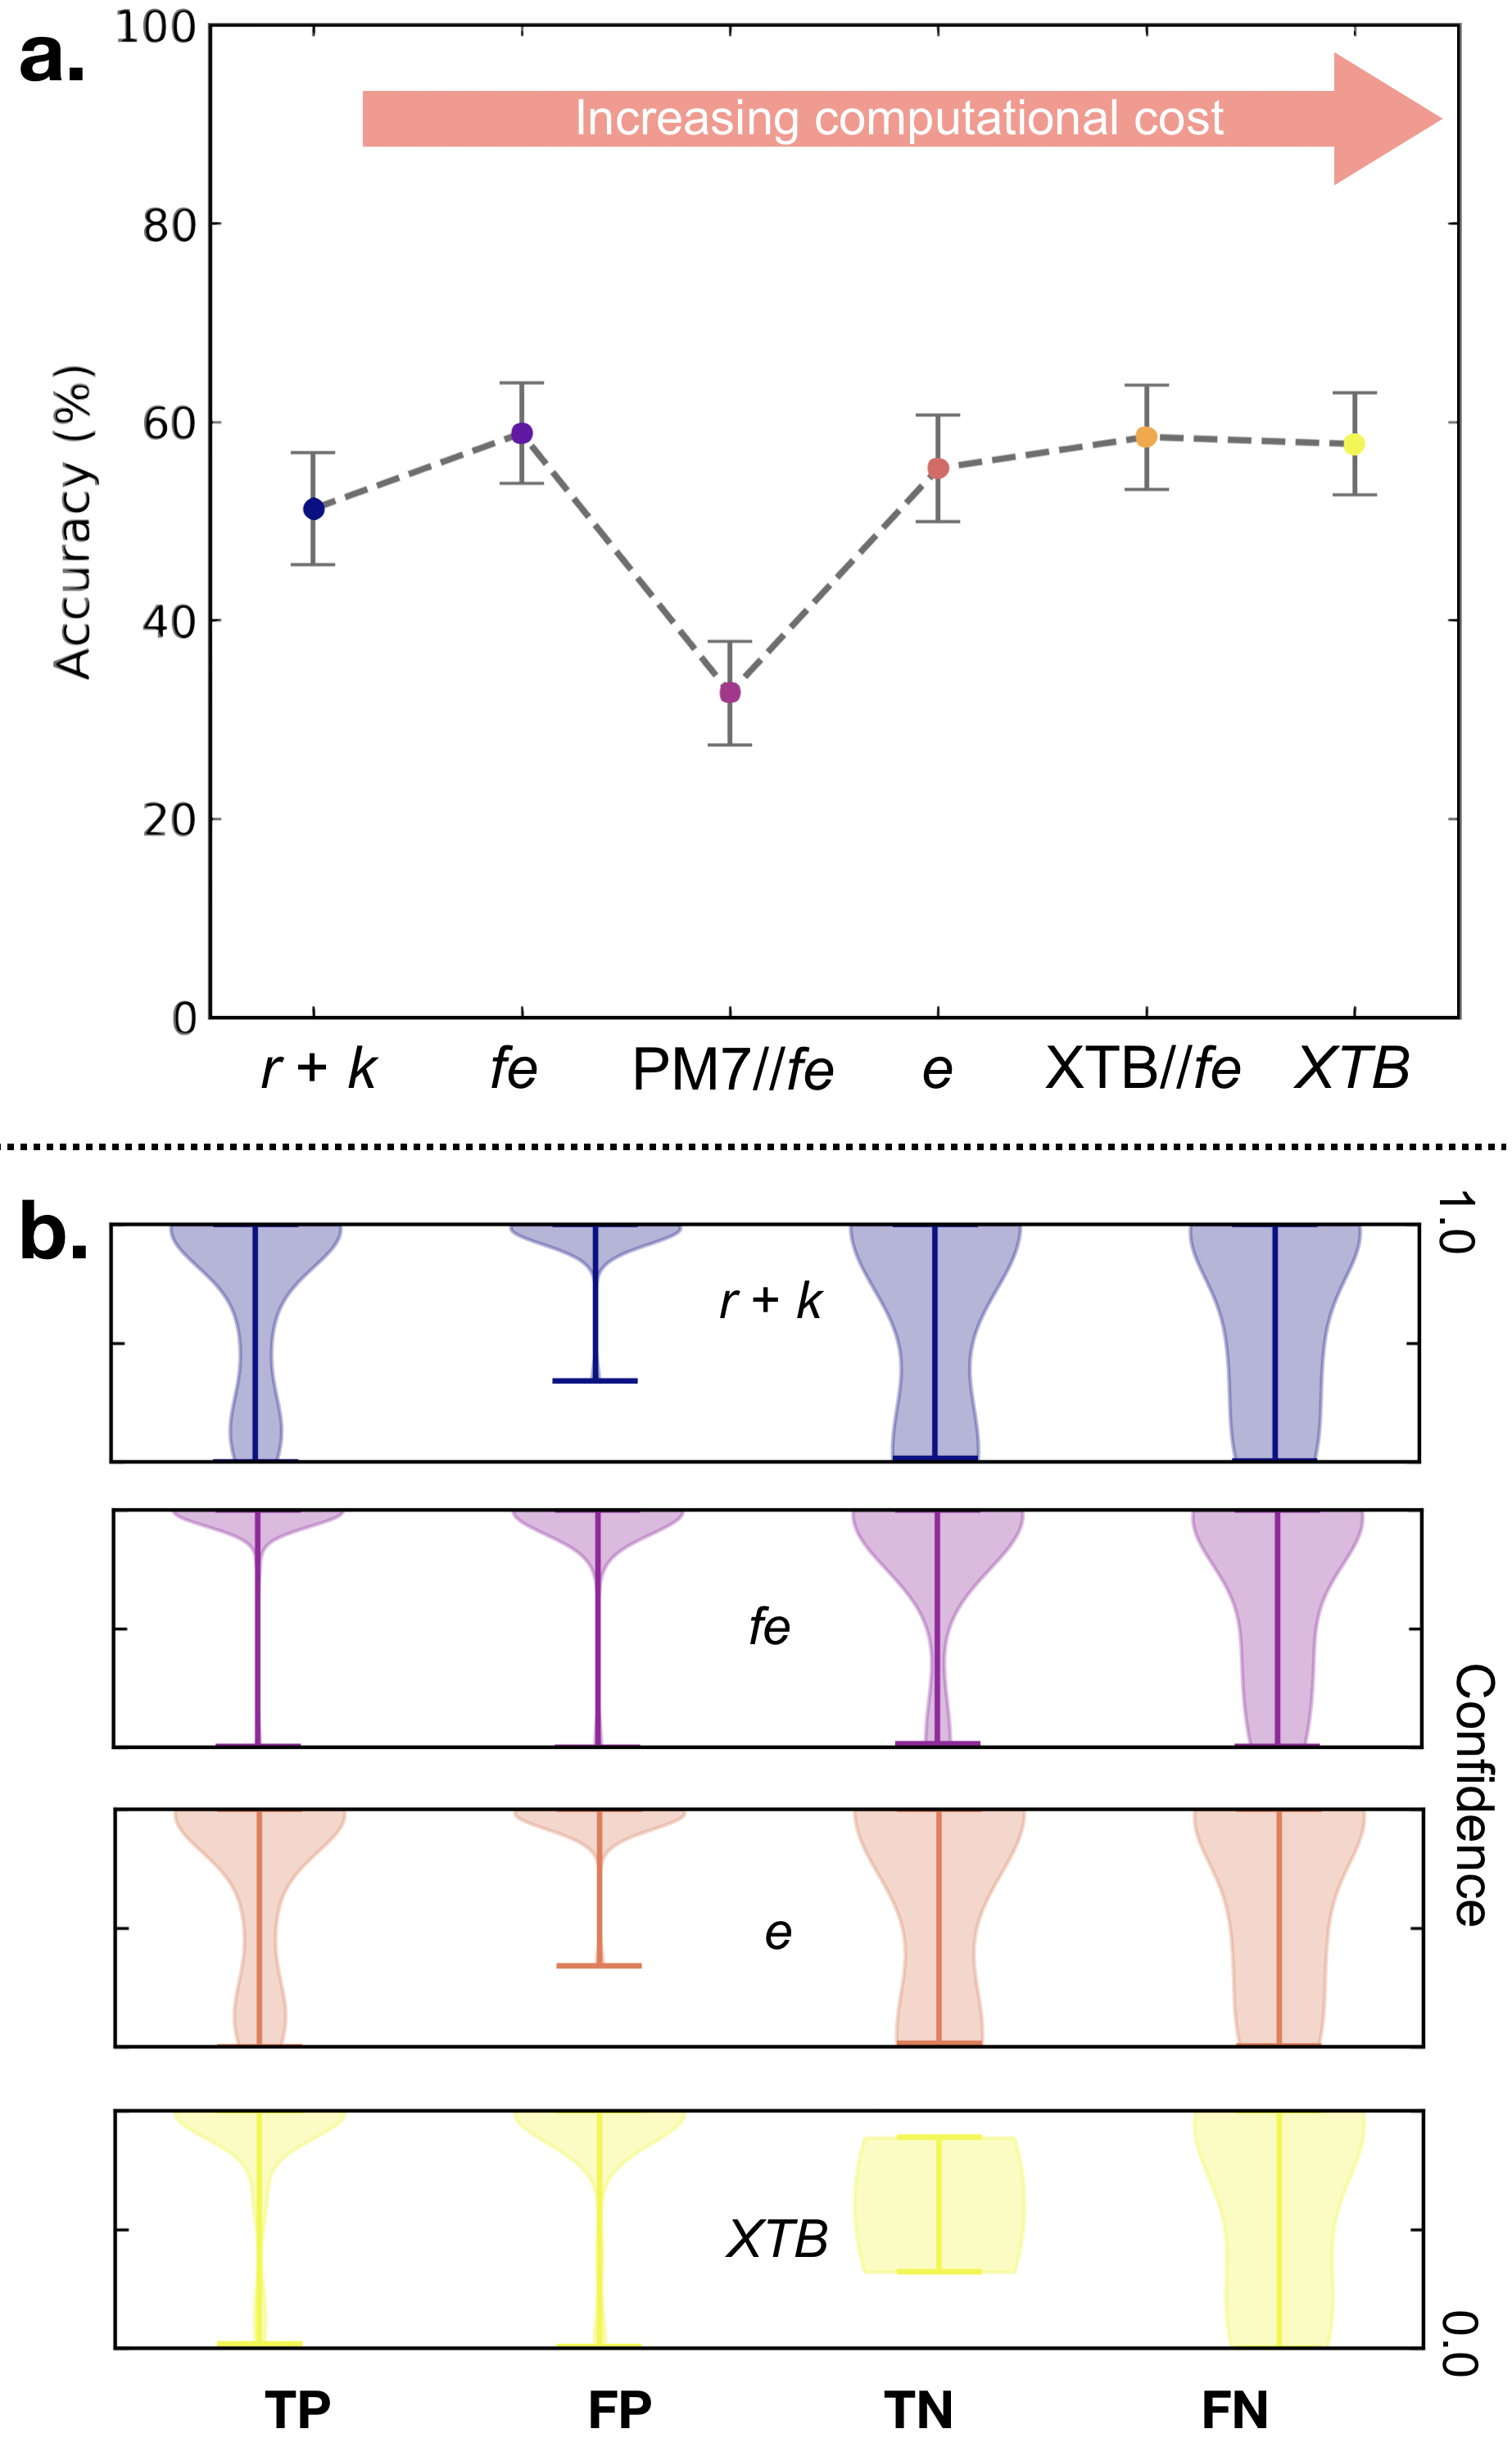
\includegraphics[width=\textwidth]{3/da//figs/fig7/fig7}
	\vspace{0.2cm}
	\hrule
	\caption{Calculated analogue activation energy ($\Delta\Delta E'_\text{CA}$, dark color) and experimentally observed catalytic efficiency ($\Delta\Delta G_\text{CA}$, light blue, only available for C-2). For C-1, the experimentally untested quinone-diene reactions are shown in bold. Two false positive for C-1 are indicated with an asterisk *. Values tabulated in Table \ref{table::si_da_20}.}
	\label{fig::da_7}
\end{figure}


Using this computationally inexpensive approach cage C-1 was found to be non-catalytic for seven out of ten reactions tested, while q1-d1 and q1-d3 combinations were within computational error. However, the substrate combination q5-d4 is clearly predicted to lead to catalysis. As this cage-substrate combination was not reported in our original work,\cite{MartCentelles2018} we have now monitored this reaction and found no obvious acceleration compared to the cage-free control experiment. This suggests that there are other subtleties involved in promoting catalysis, which will need to be explored in further studies. 

We have compared these results to those obtained using full optimization (Figure \ref{fig::si_da_30}). Selecting the set of substrates with the largest discrepancy to experiments (q1+d1 q5+d4) and q7+d2 within C-1 and C-2, we observed that the full transition states provided almost identical results to those obtained using TS analogues ($R^2 =0.94$, MAD = 0.6 \kcalx, Figure \ref{fig::si_da_30}). Moreover, the number of CPU-hours (CPUh) required to calculate a single $\Delta\Delta E$ value using TS analogues ($\sim$100 CPUh, up to 12 hours on 8 CPUs) is at least an order of magnitude lower than when using fully optimised TS ($\sim$1000 CPUh, 5 days on 8 CPUs using the TS analogues as starting point), thus demonstrating the substantial computational cost saved by our approach without compromising accuracy. 

\subsection{Conclusion}

Supramolecular metallocages have emerged as promising biomimetic catalysts. However, a theoretical understanding of the structural and electronic factor that determine efficient binding and catalysis has been lacking. Here, we have rationalized the binding and significantly different Diels-Alder catalytic activity for two highly-homologous metallocages (C-1 and C-2) through complementary classical simulations and quantum calculations. This is the first computational study that simultaneously explores binding and catalysis with multiple cage and substrate combinations. For the DA reactions studied here, we find that electronic activation of dienophile is observed for both cages. However, in the case of inactive C-1, this is offset by significant distortion energy which inhibits the interaction with the incoming diene. In contrast, catalytically active C-2 is much more able to accommodate distortion approaching the transition state. This suggests that, in addition to the catalytic machinery required to activate the substrates undergoing chemical reactions, novel metallocages designs should consider the plasticity of the building blocks and the cage as a whole. While these features are now understood in enzyme catalysis, they have been much less studied in biomimetic catalyst design.

In addition to rationalising the catalytic activity, this work introduces an efficient computational protocol to model metallosupramolecular catalysts in solution. Further work is underway to automate this process within an open-source Python module (cgbind, {\url{https://github.com/duartegroup/cgbind}}). We expect this to motivate a closer interaction between experimentalists and computational chemists in the quest towards the discovery of novel catalysts. 


\subsection{Computational Methods}

{\bfseries{MD Simulations}}. Configurational sampling of the cage structures in dichloromethane (DCM) was performed using classical MD simulations. For ligands and substrates, OPLS-AA-compatible force-field parameters were generated using the Macromodel ffld14 version (Schrödinger LCC).\cite{MacroModel} Restrained electrostatic potential (RESP) charges were derived by fitting partial charges to HF/6-31G(d) electrostatic potentials calculated using Gaussian 09 (version D.01).\cite{G09} Geometries for these calculations were obtained from optimisations at the TPSS-D3BJ/def2TZVP/fit level of theory. The topology for DCM was taken from the GROMACS Molecule \& Liquid Database.\cite{vanderSpoel2012}
All simulations were performed using the GROMACS package (version 2019.1)\cite{Abraham2015} using three-dimensional periodic boundary conditions. Long-range electrostatic interactions were treated using the particle mesh Ewald (PME) approach\cite{Darden1993} with a cut-off length of 1.0 nm. A dispersion correction was applied to energy and pressure terms to account for truncation of van der Waals terms.
The systems were immersed in a box of solvent with a distance from the border of at least 15 \AA. Following steepest descent minimization, the systems were equilibrated in two steps; the first phase involved simulating for 100 ps under a constant volume ($NVT$) ensemble with position restraints applied to heavy atoms. The temperature was maintained at 298 K using the velocity-rescale method. This was followed by 100 ps of constant-pressure ($NPT$) equilibration using the Parrinello–Rahman pressure coupling algorithm with the compressibility set to 4.5 × 10${}^{–5}$ bar${}^{-1}$ and the time constant set to 5 ps. A 1 fs time step was used during these stages to allow potential inhomogeneities to self-adjust. Each system was then equilibrated initially for 10 ns with a 1 fs time step at constant pressure. Three different runs, differing in the initial random seed were run per system. The first 1 ns was removed from the analysis.

{\bfseries{Electronic Structure Calculations}}. All density functional theory (DFT) calculations were performed in the ORCA v. 4.1 software package.\cite{Neese2017} Initial geometry optimisations for cages (C-1, C-2) and cage–substrate complexes (bq$\subset$C-1, bq$\subset$C-2) were performed with the M06-2X functional,\cite{Zhao2007} the Ahlrichs def2-TZVP\cite{Weigend2005, Weigend2006} basis set which includes the ECP28MWB81 on Pd. Solvent effects were accounted for with the SMD\cite{Marenich2009} solvent model with parameters appropriate for DCM. Subsequent optimisations were performed with the PBE0\cite{Adamo1999} functional with the Becke-Johnson damped D3 dispersion correction (D3BJ)\cite{Johnson2006} in combination with a def2-SVP basis set. Where stated vibrational frequencies were computed at the optimization level of theory to confirm whether the structures correspond to minima or a transition states and to evaluate the zero-point vibrational energy (ZPE) and thermal corrections at 298 K. Gibbs free energies in which a change of molecularity occurs include a 1 atm to 1 M standard state correction. 
Single-point energies were obtained at the M06-2X/def2-TZVP level of theory in DCM solvent using the SMD solvent model. Single point energies for non-catalysed DA reactions have also been carried out using PBE0,\cite{Adamo1999} TPSS,\cite{TPSS} PW6B95,\cite{Zhao2005} $\omega$B97X-D3\cite{Chai2008} and M06-2X\cite{Zhao2007} functionals to analyse the influence of the functional and dispersion upon optimized structures and stabilities when compared to the DLPNO-CCSD(T)\cite{Riplinger2016} linear-scaling coupled cluster implementation, which was used in combination with the minimally augmented doubly polarized ma-def2-TZVPP basis set. The chain of spheres resolution of identity (RIJCOSX in ORCA) approximation was used for the Hartree-Fock exchange component of hybrid functionals, with the default fitting bases. NBO charge and second order perturbation analyses were carried out in NBO\cite{Glendening2013} v. 6.0. Multiwfn v. 3.6\cite{Lu2011} has been used for electron density analysis. Unless specified otherwise, all energy differences are calculated at SMD(DCM)-M06-2X/def2-TZVP//PBE0-D3BJ/def2-SVP level of DFT theory.


\clearpage
\section{Selected Supporting Information I}
\emph{Full Supporting Information including raw data can be found at:}\\ {\url{https://pubs.acs.org/doi/abs/10.1021/jacs.9b10302}}


\subsection{Square-planar Metal Model}
\label{section::da_si_1_1}

The square planar palladium dummy atom model originally presented by Fujita et al. was used for all MD simulations.\cite{Yoneya2012} This model is based on previous work on transition metal parameterization by Aqvist and Warshel.\cite{Aaqvist1990} The model consists of four particles, each of them possessing a charge of +0.5, while the central particle possesses zero charge. The geometry of the dummy complex itself is kept rigid by the imposition of large force constants on the metal–dummy bonds (Table \ref{table::si_da_1}). However, as there are no bonds between the dummy complex and the surrounding ligands, overall rotation is allowed, and no internal forces are associated with such rotation. This means that the system is free to exchange ligands on the relevant time scale. 


\begin{table}[h]
	\def\arraystretch{1.7}
	\begin{tabularx}{\textwidth}{YYYYY}
		\hline
		\multicolumn{5}{c}{van der Waals}\\
		\hline
		
		name &	Mass / amu&	Charge / $e$& $\sigma$ / nm&	$\epsilon$ / kJ mol$^{–1}$\\
		M  &   	98.336&	0.0	&0.1718	&2.89951
 \\
		D$_{i/j}$ &	2.016&	0.500&	0.0	&0.0
\\
		
		\hline
		\multicolumn{3}{c}{Bond}&&\\
		
		          &  $r_0$ / nm	& \multicolumn{2}{c}{$K_b$ / kJ mol$^{–1}$}
&\\
		D$_{i/j}$--M&	0.09&	\multicolumn{2}{c}{669440}
&\\
		
		\hline
		\multicolumn{3}{c}{Angle}&&\\
		
		& $\theta$ / degrees&		\multicolumn{2}{c}{$K_\theta$ / kJ mol$^{-1}$ rad$^{-2}$}
&\\
		D$_{i}$-M-D$_{j}$(trans)	&180&	\multicolumn{2}{c}{2092}&\\
		D$_{i}$-M-D$_{j}$(cis)	&90	&\multicolumn{2}{c}{2092}&\\

	\end{tabularx}
	\hrule
	\vspace{0.2cm}
	\caption{Force Field Parameters for the Pd dummy model used in this work. Definitions appropriate for the GROMACS simulation package.}
	\label{table::si_da_1}
\end{table}

The modified Fujita parameters a Pd(II) were initially tested in water, employing the three-point transferable intermolecular potential (TIP3P).\cite{Jorgensen1983} The system was simulated for 5 ns and the Pd–O distance obtained from analysis of the radial distribution function (RDF, Figure \ref{fig::si_da_1}). The modal distance is somewhat shorter than the experimental value (1.85 \AA$\;$ cf. expt.\cite{Persson2010} 2.01 \AA).


\begin{figure}[h!]
	\vspace{0.4cm}
	\centering
	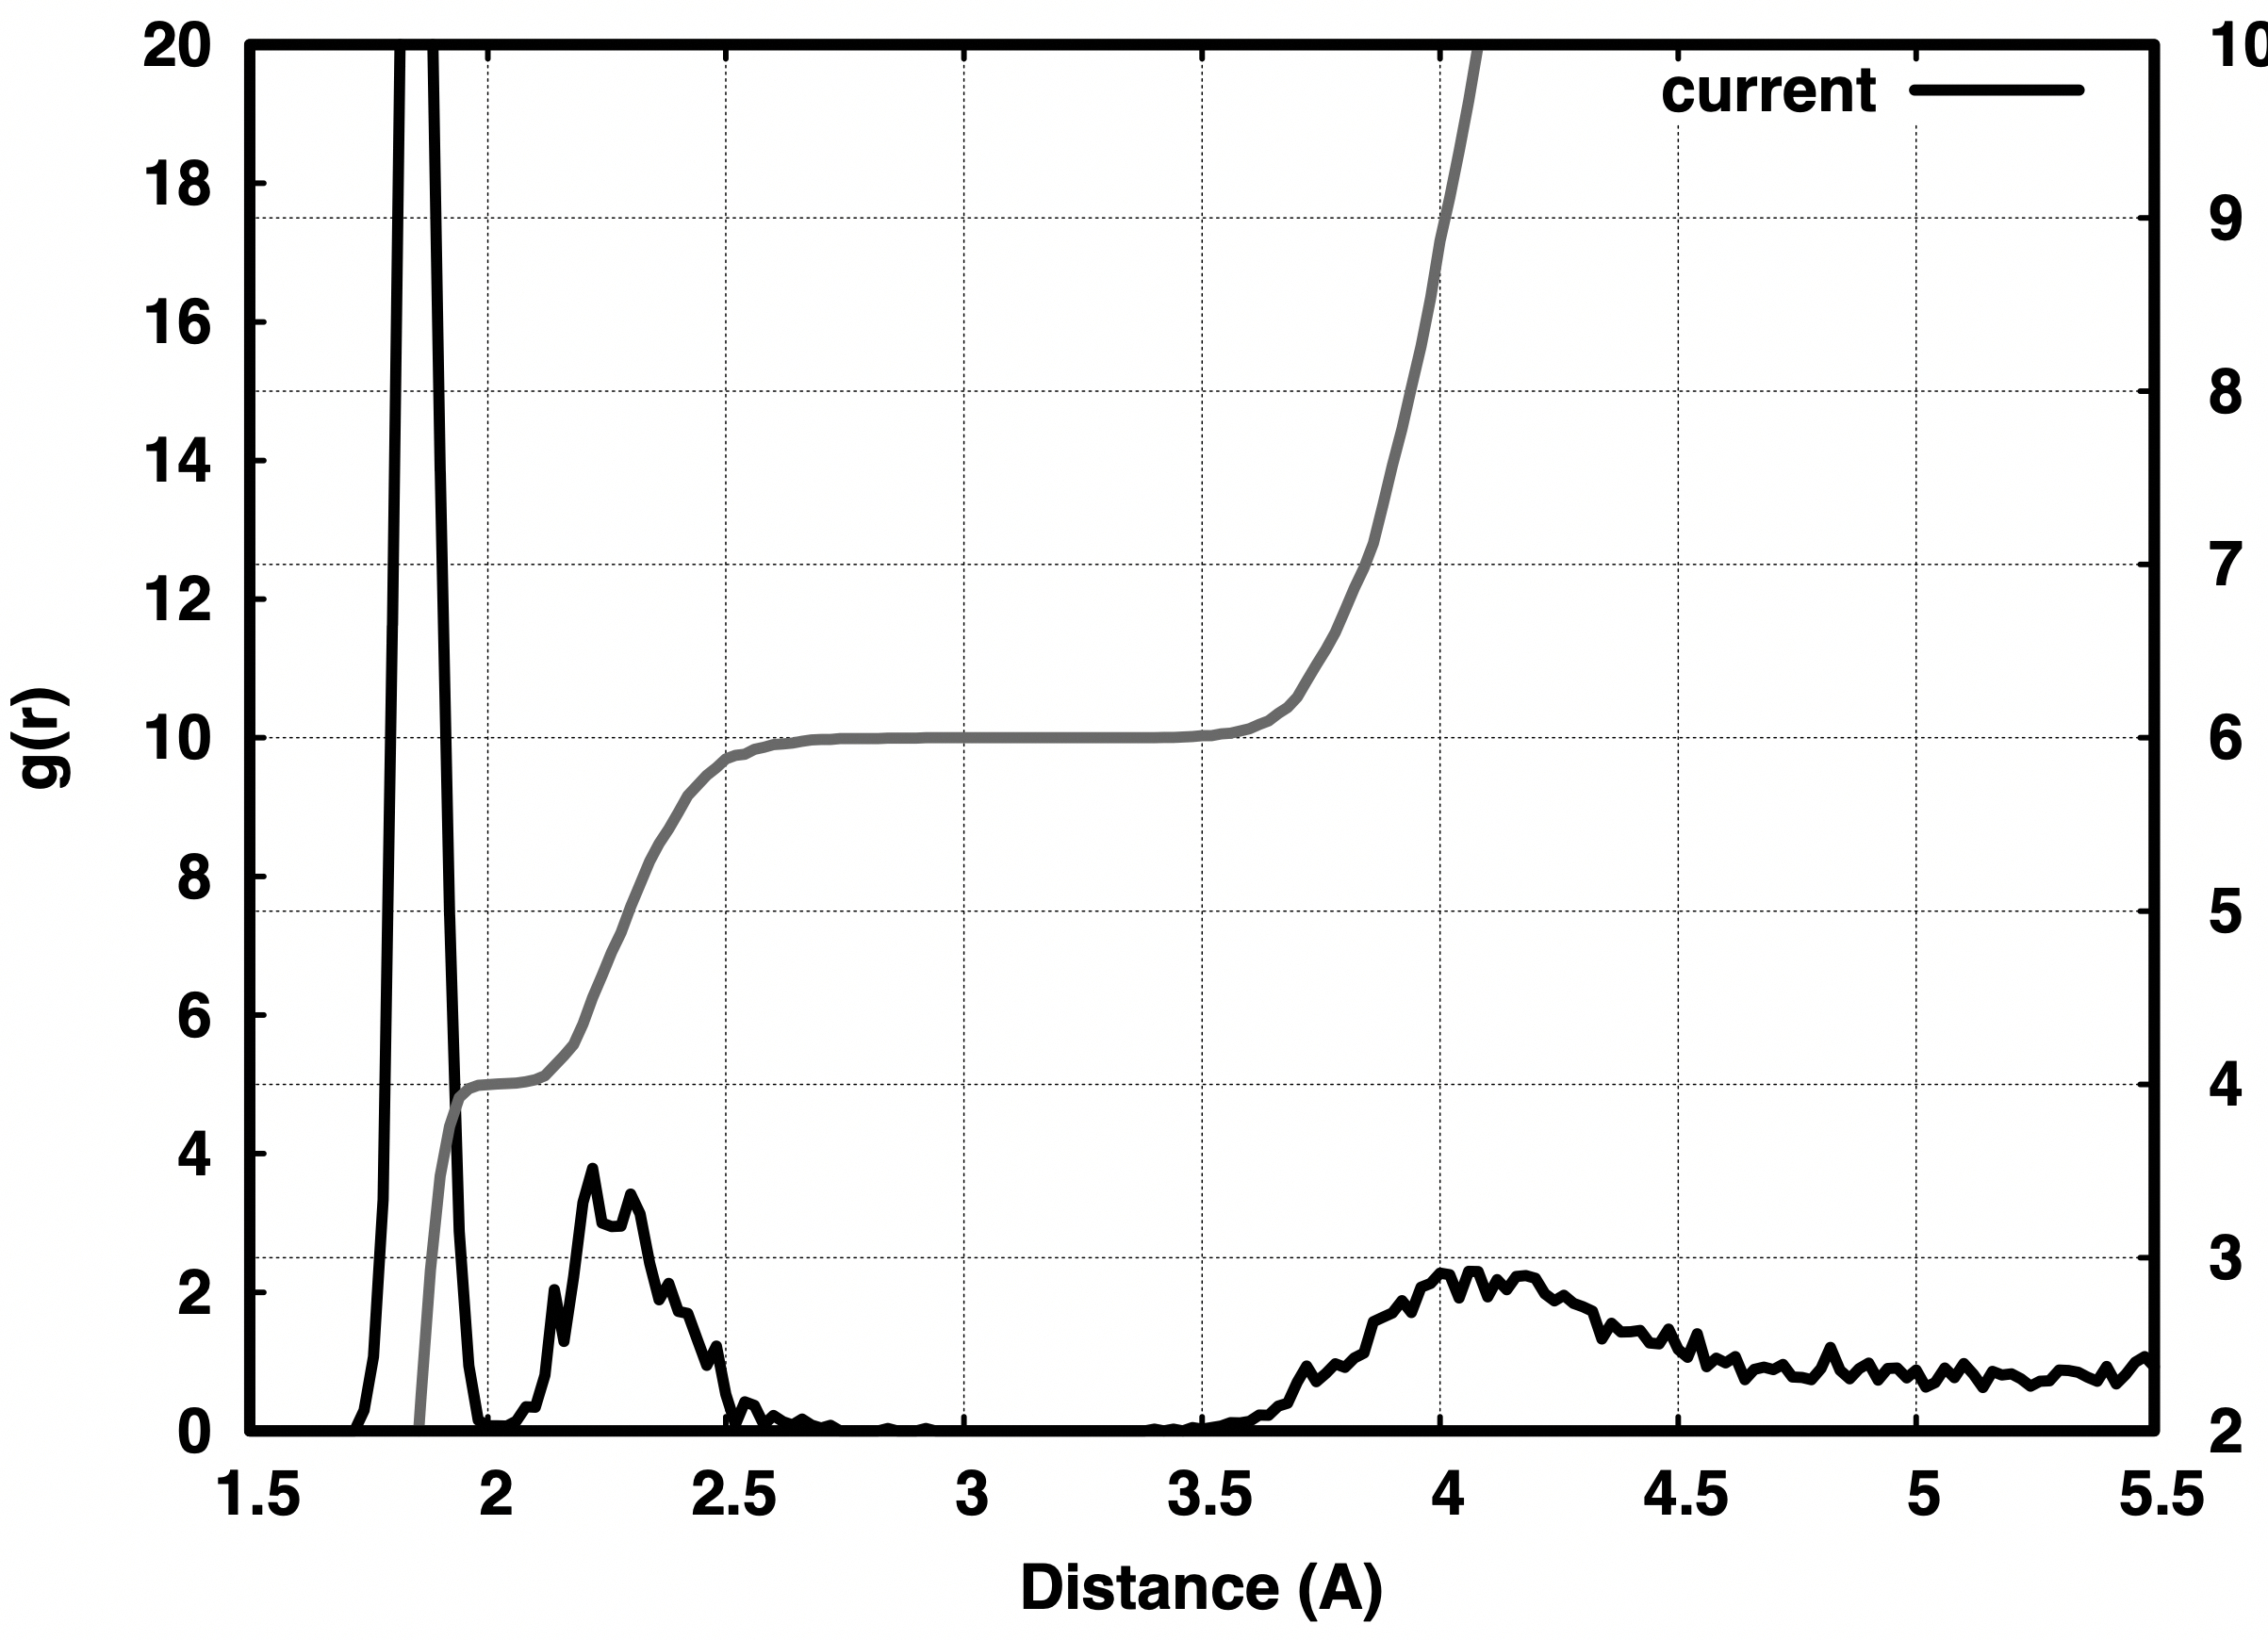
\includegraphics[width=10cm]{3/da//figs/figS1}
	\vspace{0.2cm}
	\hrule
	\caption{Pd–O radial distribution function [$g(r)$] for a Pd(II) ion in a cubic box balanced with two Cl$^{-}$ ions at 298.15 K from a 5 ns MD trajectory. Simulation set up by Prof. Fernanda Duarte.}
	\label{fig::si_da_1}
\end{figure}


\subsection{Metallocage MD Modelling}
\label{section::da_si_1_2}

\begin{figure}[h!]
	\vspace{0.4cm}
	\centering
	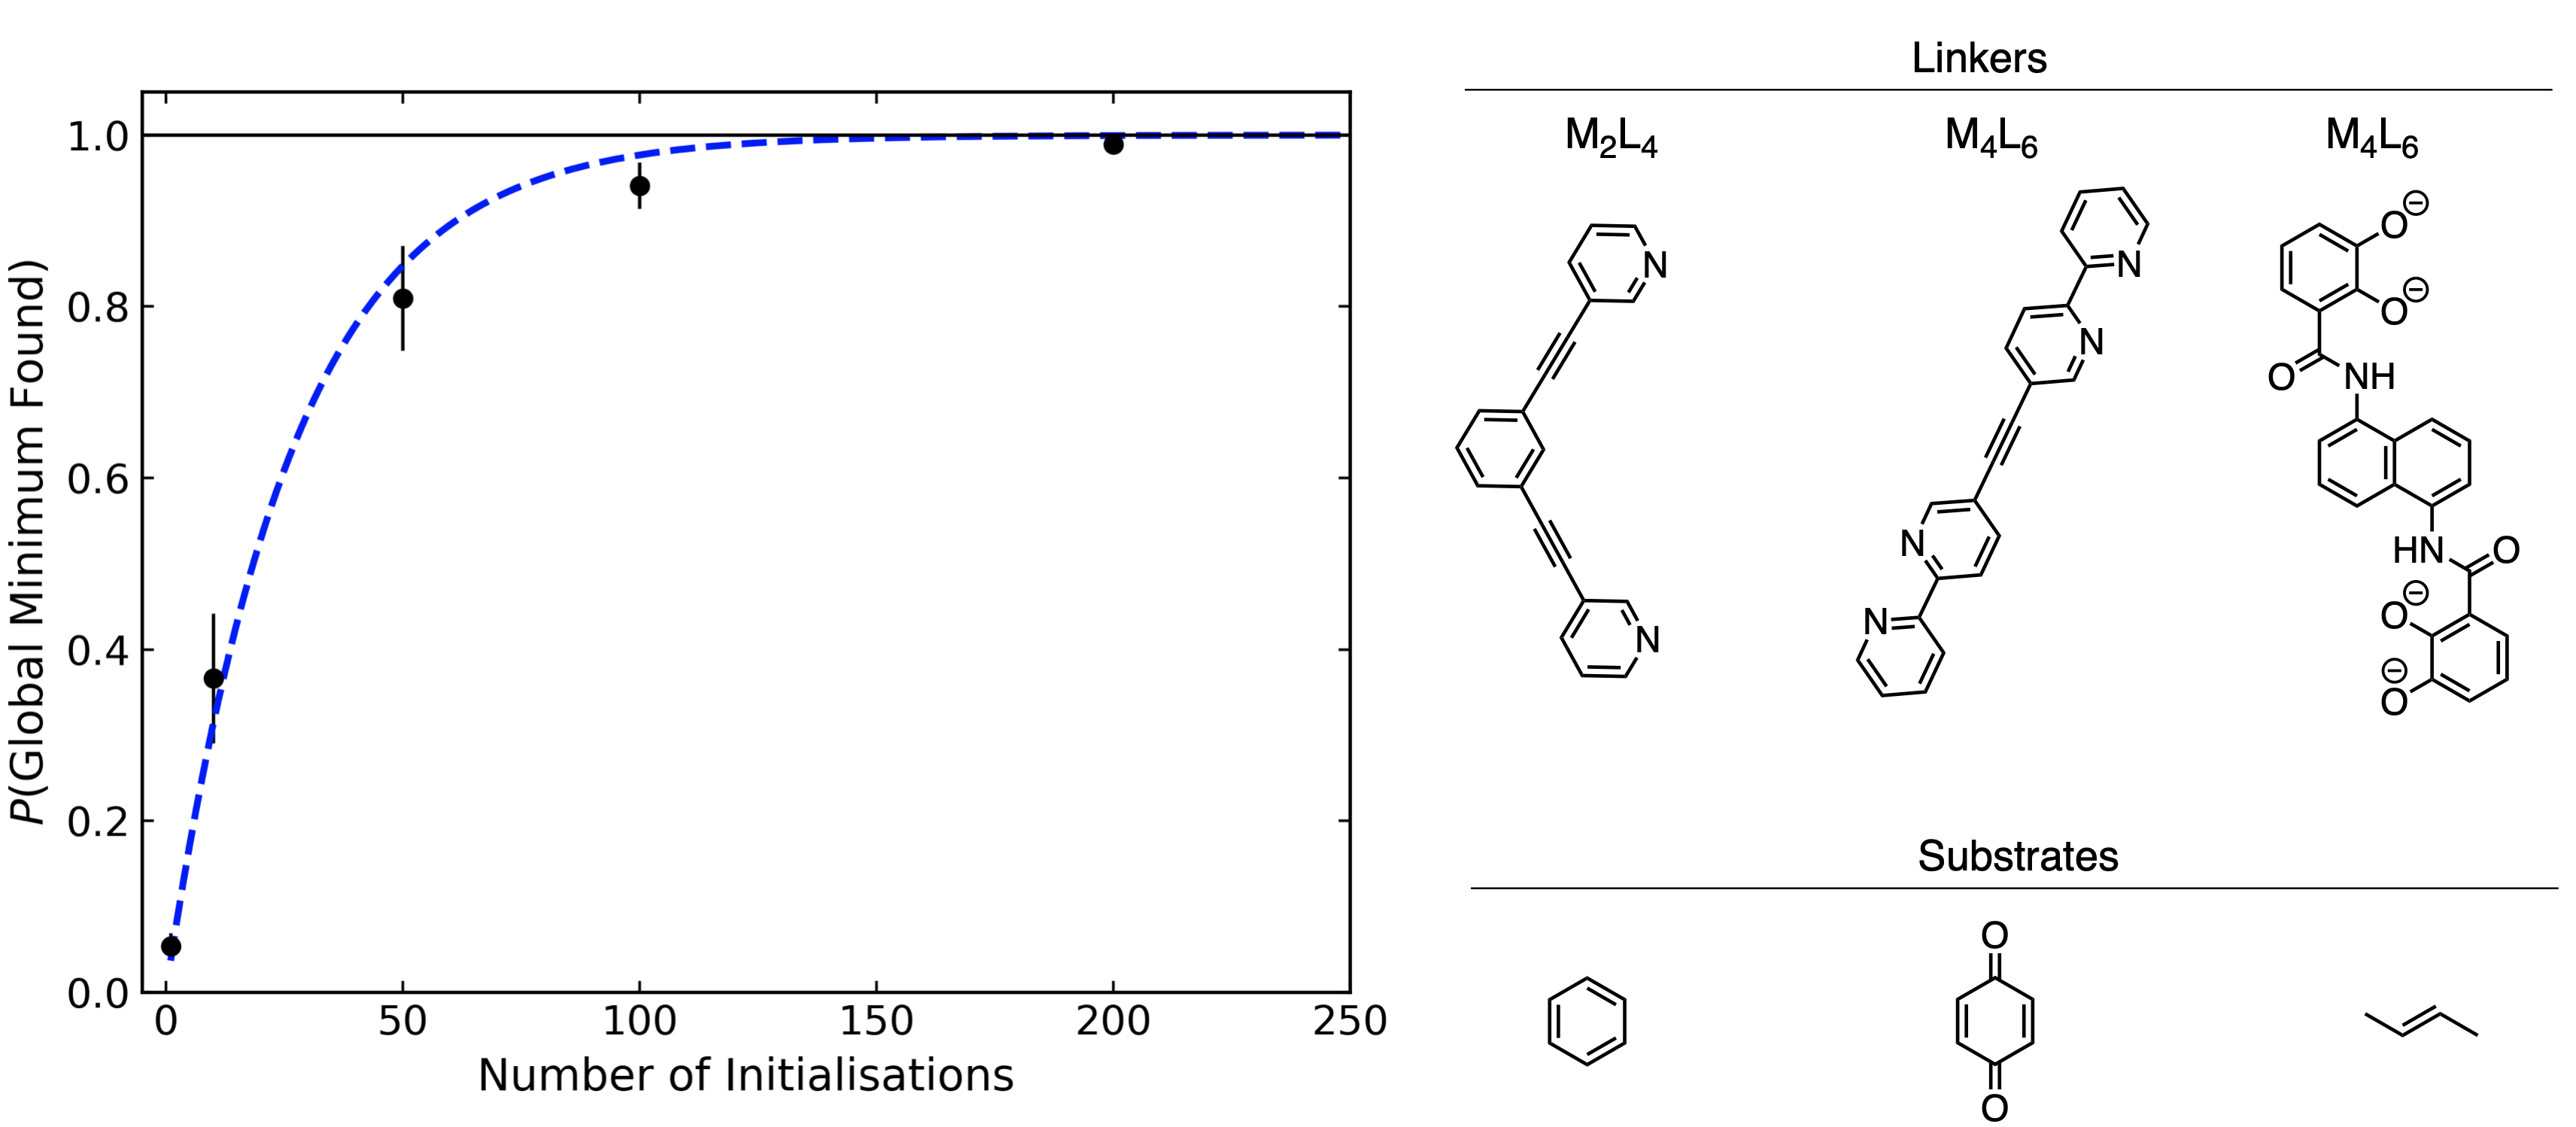
\includegraphics[width=\textwidth]{3/da//figs/figS2}
	\vspace{0.2cm}
	\hrule
	\caption{Temporal Pd–N(donor) distance variation. The solid line corresponds to a 20-step block average over 3 replicas and the shaded area the range of the block.}
	\label{fig::si_da_2}
\end{figure}


\begin{figure}[h!]
	\vspace{0.4cm}
	\centering
	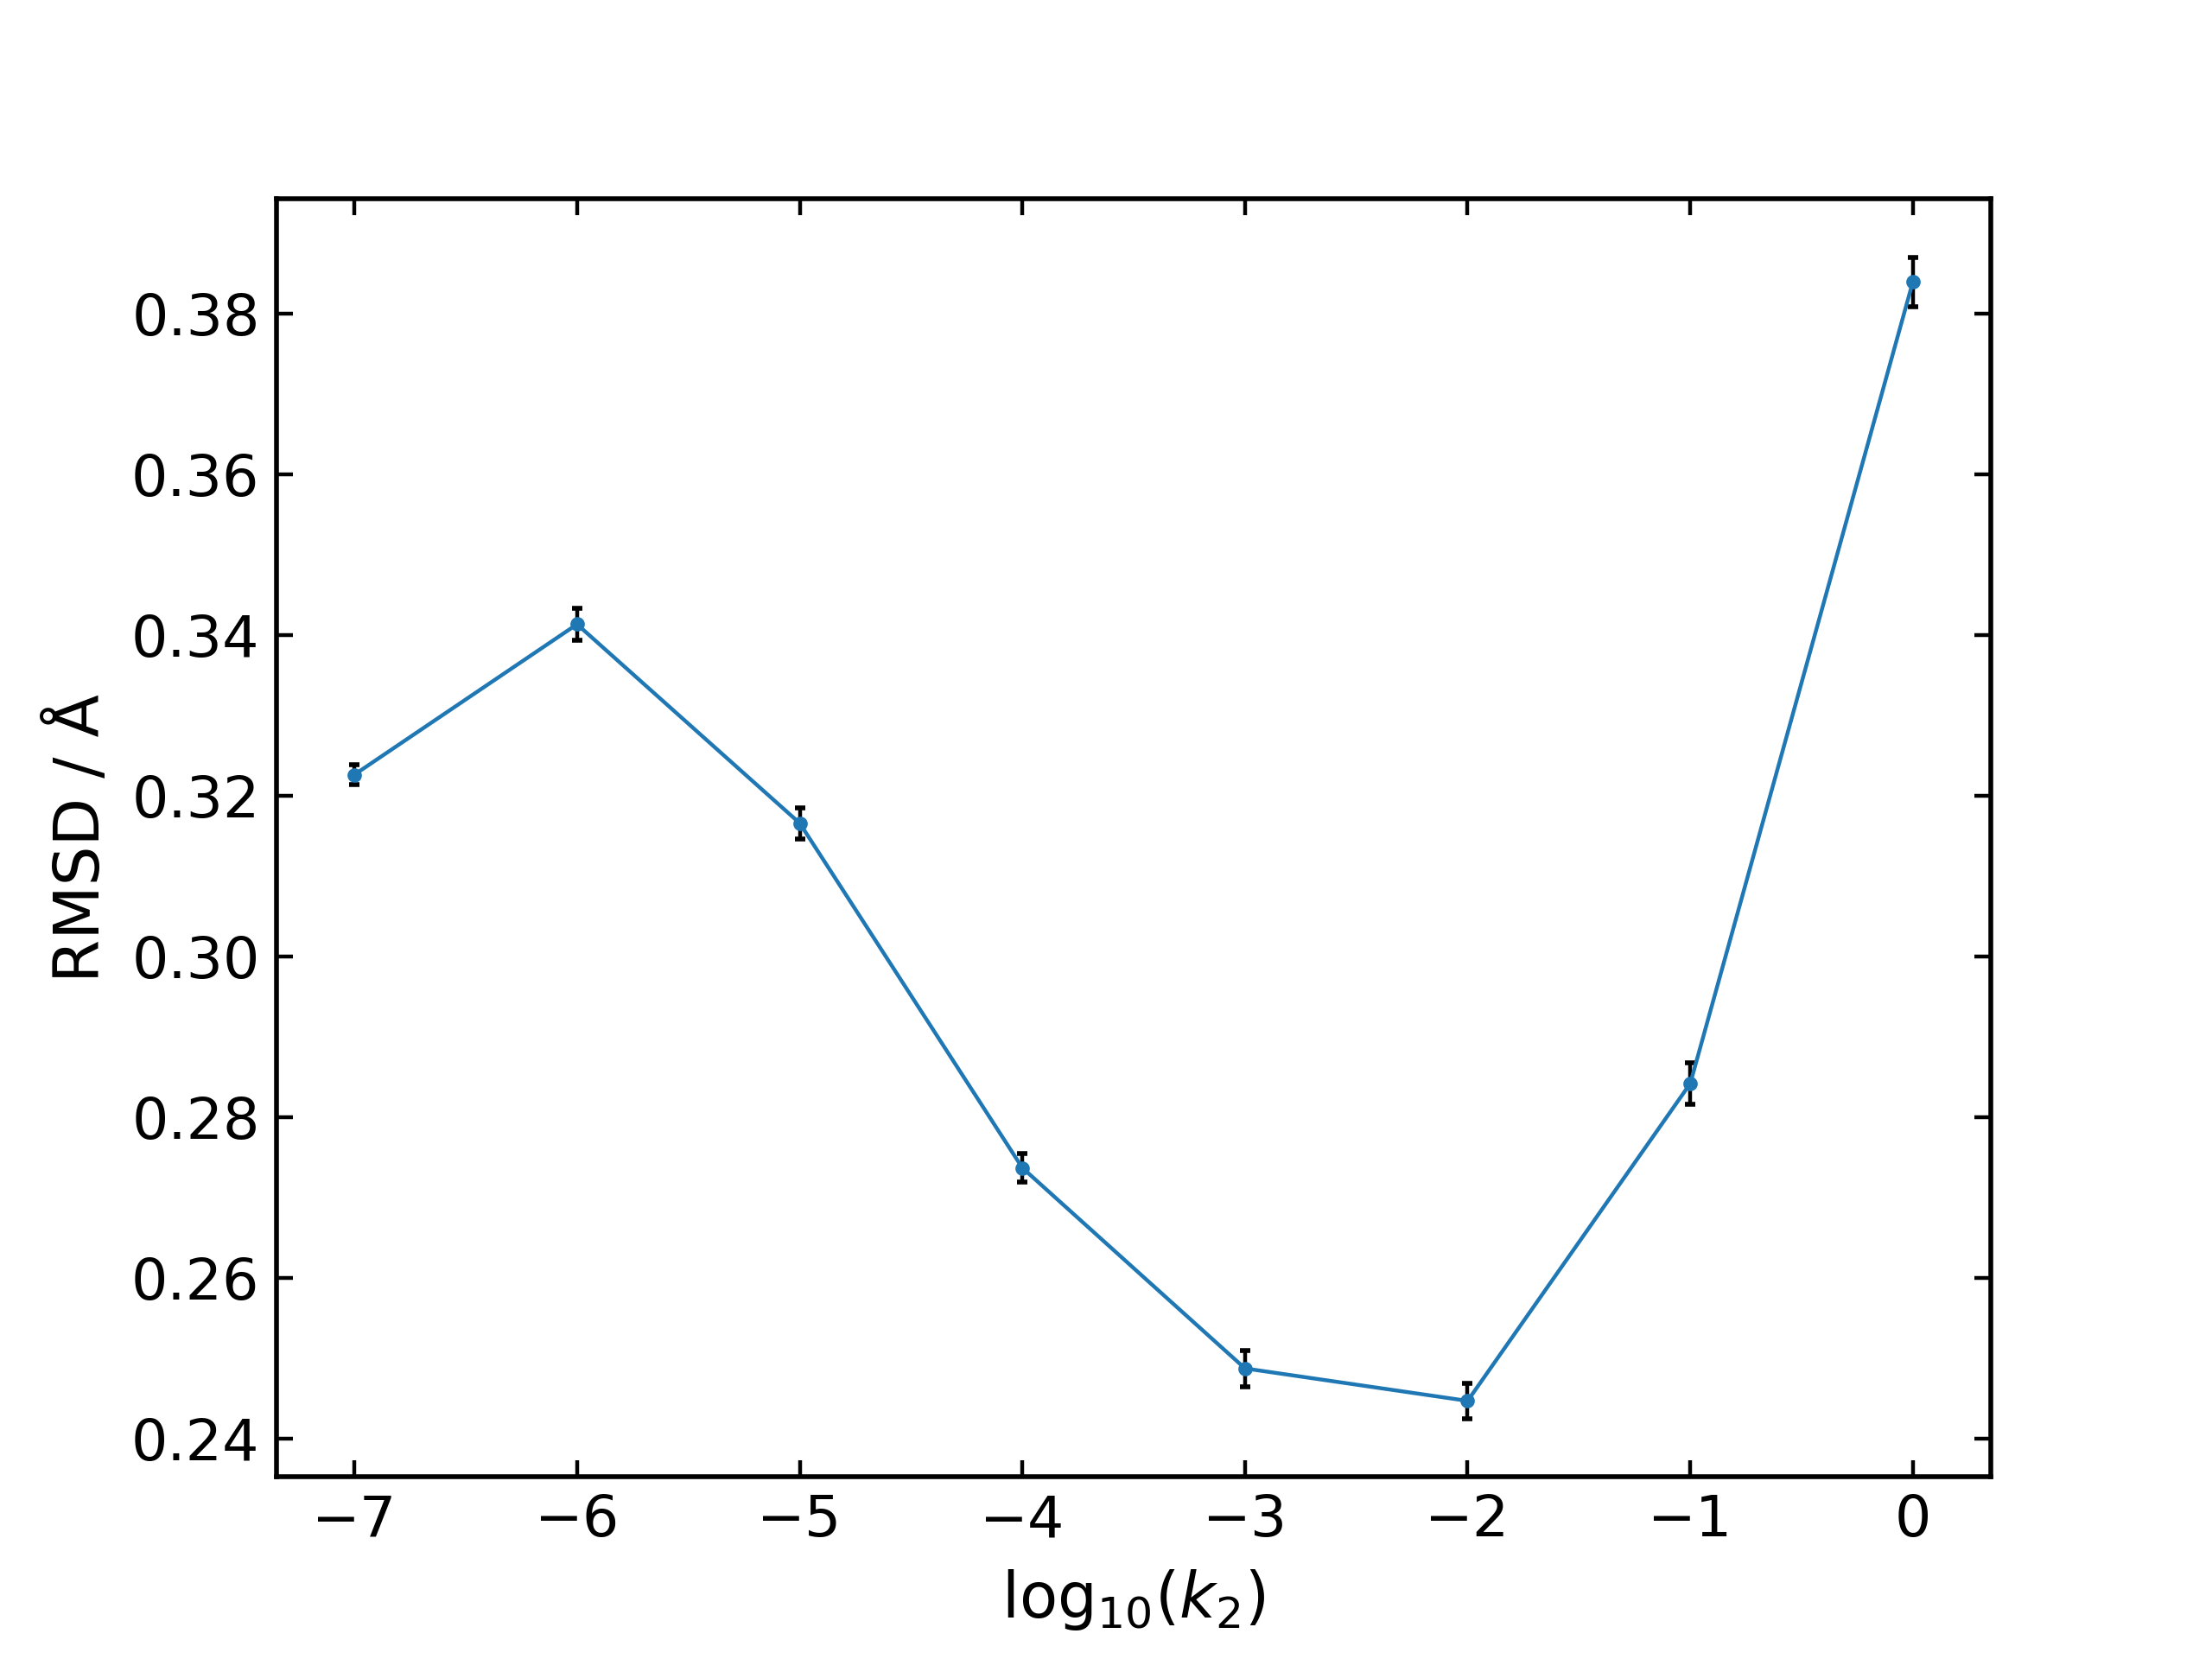
\includegraphics[width=\textwidth]{3/da//figs/figS3}
	\vspace{0.2cm}
	\hrule
	\caption{Temporal Pd–Pd distance variation. The solid line corresponds to a 20-step block average over 3 replicas and the shaded area the range of the block.}
	\label{fig::si_da_3}
\end{figure}

\begin{figure}[h!]
	\vspace{0.4cm}
	\centering
	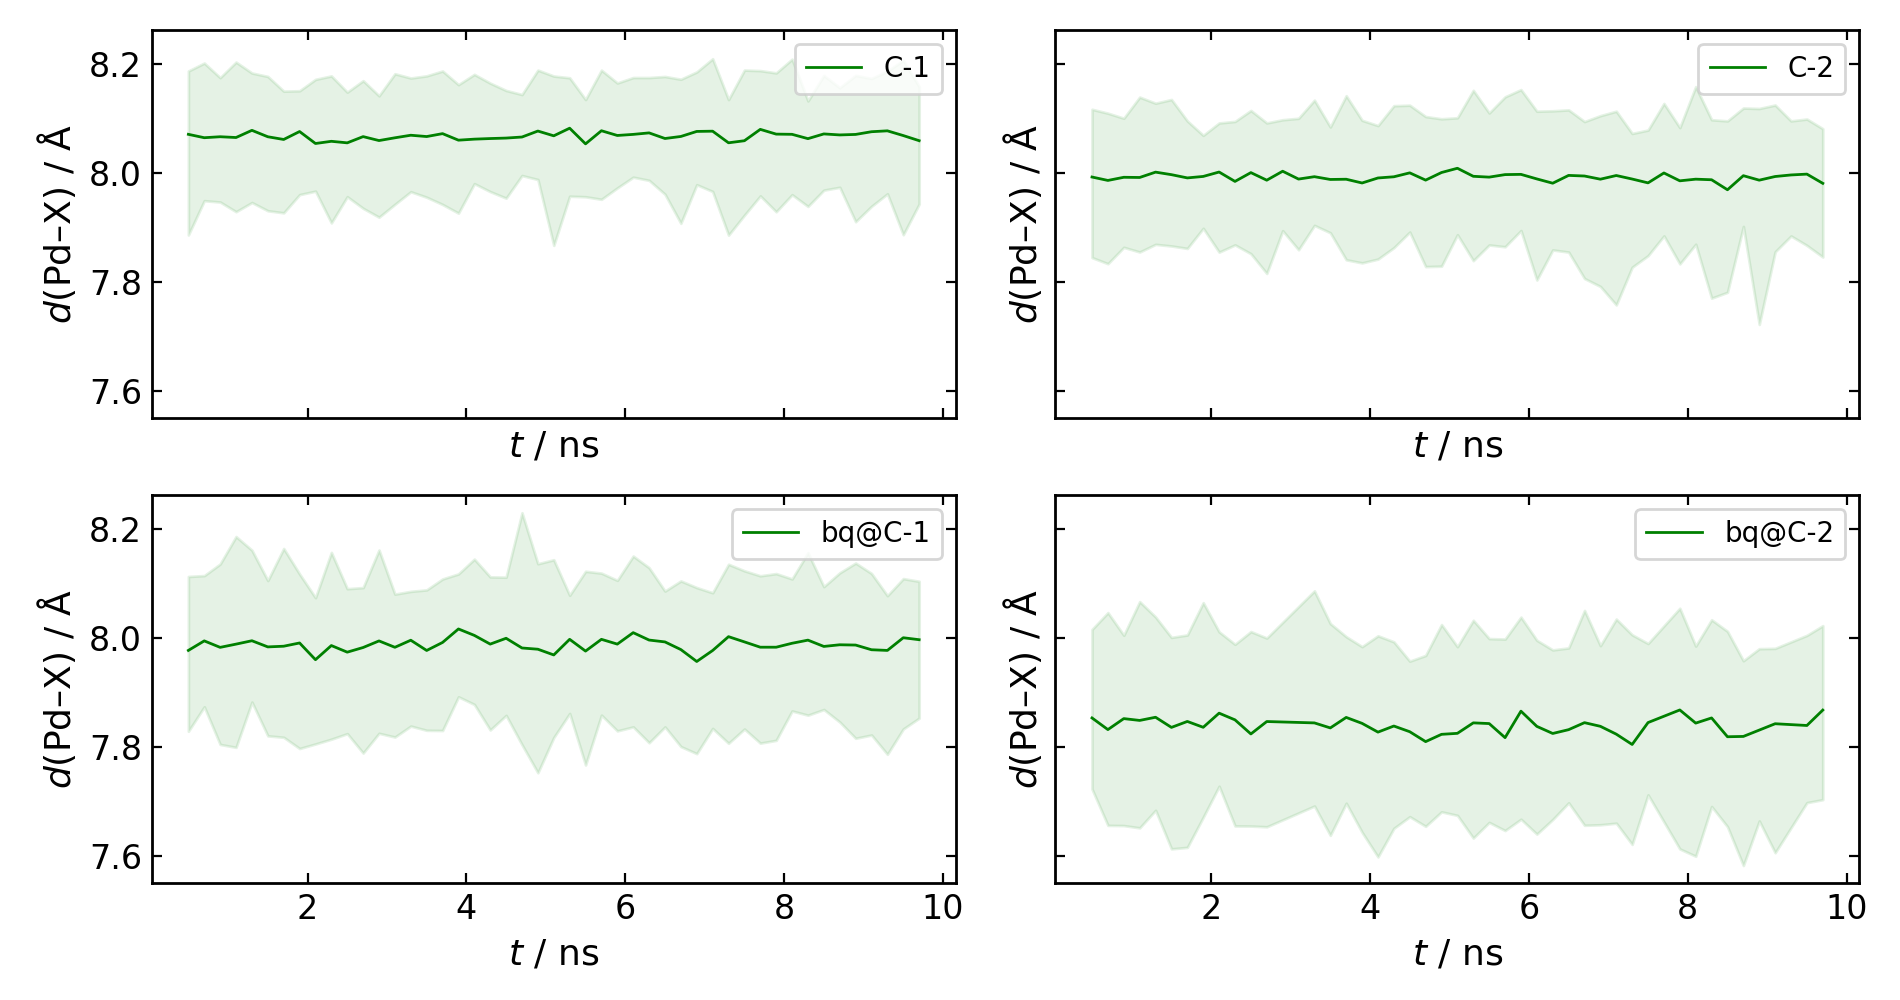
\includegraphics[width=\textwidth]{3/da//figs/figS4}
	\vspace{0.2cm}
	\hrule
	\caption{Temporal Pd–X distance variation, where X=CH, N for C-1 and C-2 respectively. The solid line corresponds to a 20-step block average over 3 replicas and the shaded area the range of the block.}
	\label{fig::si_da_4}
\end{figure}


\begin{table}[h]
	\def\arraystretch{1.7}
	\begin{tabularx}{\textwidth}{YYYY}
		\hline		
		Species &	Description	&Distance / \AA&	Ref. distance / \AA \\
		\hline
		
			  & Pd–N&	1.954±0.002	&2.02±0.01$^a$
\\
		 C-1 &        	Pd–Pd&	12.111±0.029&	11.85$^a$
\\
			&	Pd–X	&8.067±0.007	&7.99±0.11$^a
$\\
						&	Pd–N&	1.957±0.002	&2.02±0.00$^b$
\\
		bq$\subset$C-1	&	Pd–Pd	&11.771±0.043&	12.21$^b$
\\
			&	Pd–X&	7.987±0.011	&8.02±0.17$^b$
\\
		&Pd–N&	1.952±0.002	&2.02±0.01$^c$
\\
			C-2		&Pd–Pd	&11.738±0.032	&11.50$^c
$\\
				&Pd–X	&7.991±0.007&	7.96±0.17$^c$
\\
			&Pd-N&	1.961±0.001	
&\\
			bq$\subset$C-2	&Pd–Pd	&10.960±0.052&	NA
\\
				&Pd–X&	7.83±0.015	&
\\
	
	\end{tabularx}
	\hrule
	\vspace{0.2cm}
	\caption{Average key distances for C-1, C-2, bq$\subset$C-1 and bq$\subset$C-2 calculated from MD simulations. Standard deviations in the block averages through the trajectory are given. NA = not available. a) OTf$\subset$C-1[OTf]. CCDC: 768969. Ref \cite{Liao2010}; b) [pentacenedione$\subset$C-1][OTf]4. CCDC: 1492902. Ref. \cite{August2016}; c) [C-2][SbF$_6^{-}$]$_2$. CCDC: 853226. Ref. \cite{Lewis2012}.}
	\label{table::si_da_2}
\end{table}


\begin{figure}[h!]
	\vspace{0.4cm}
	\centering
	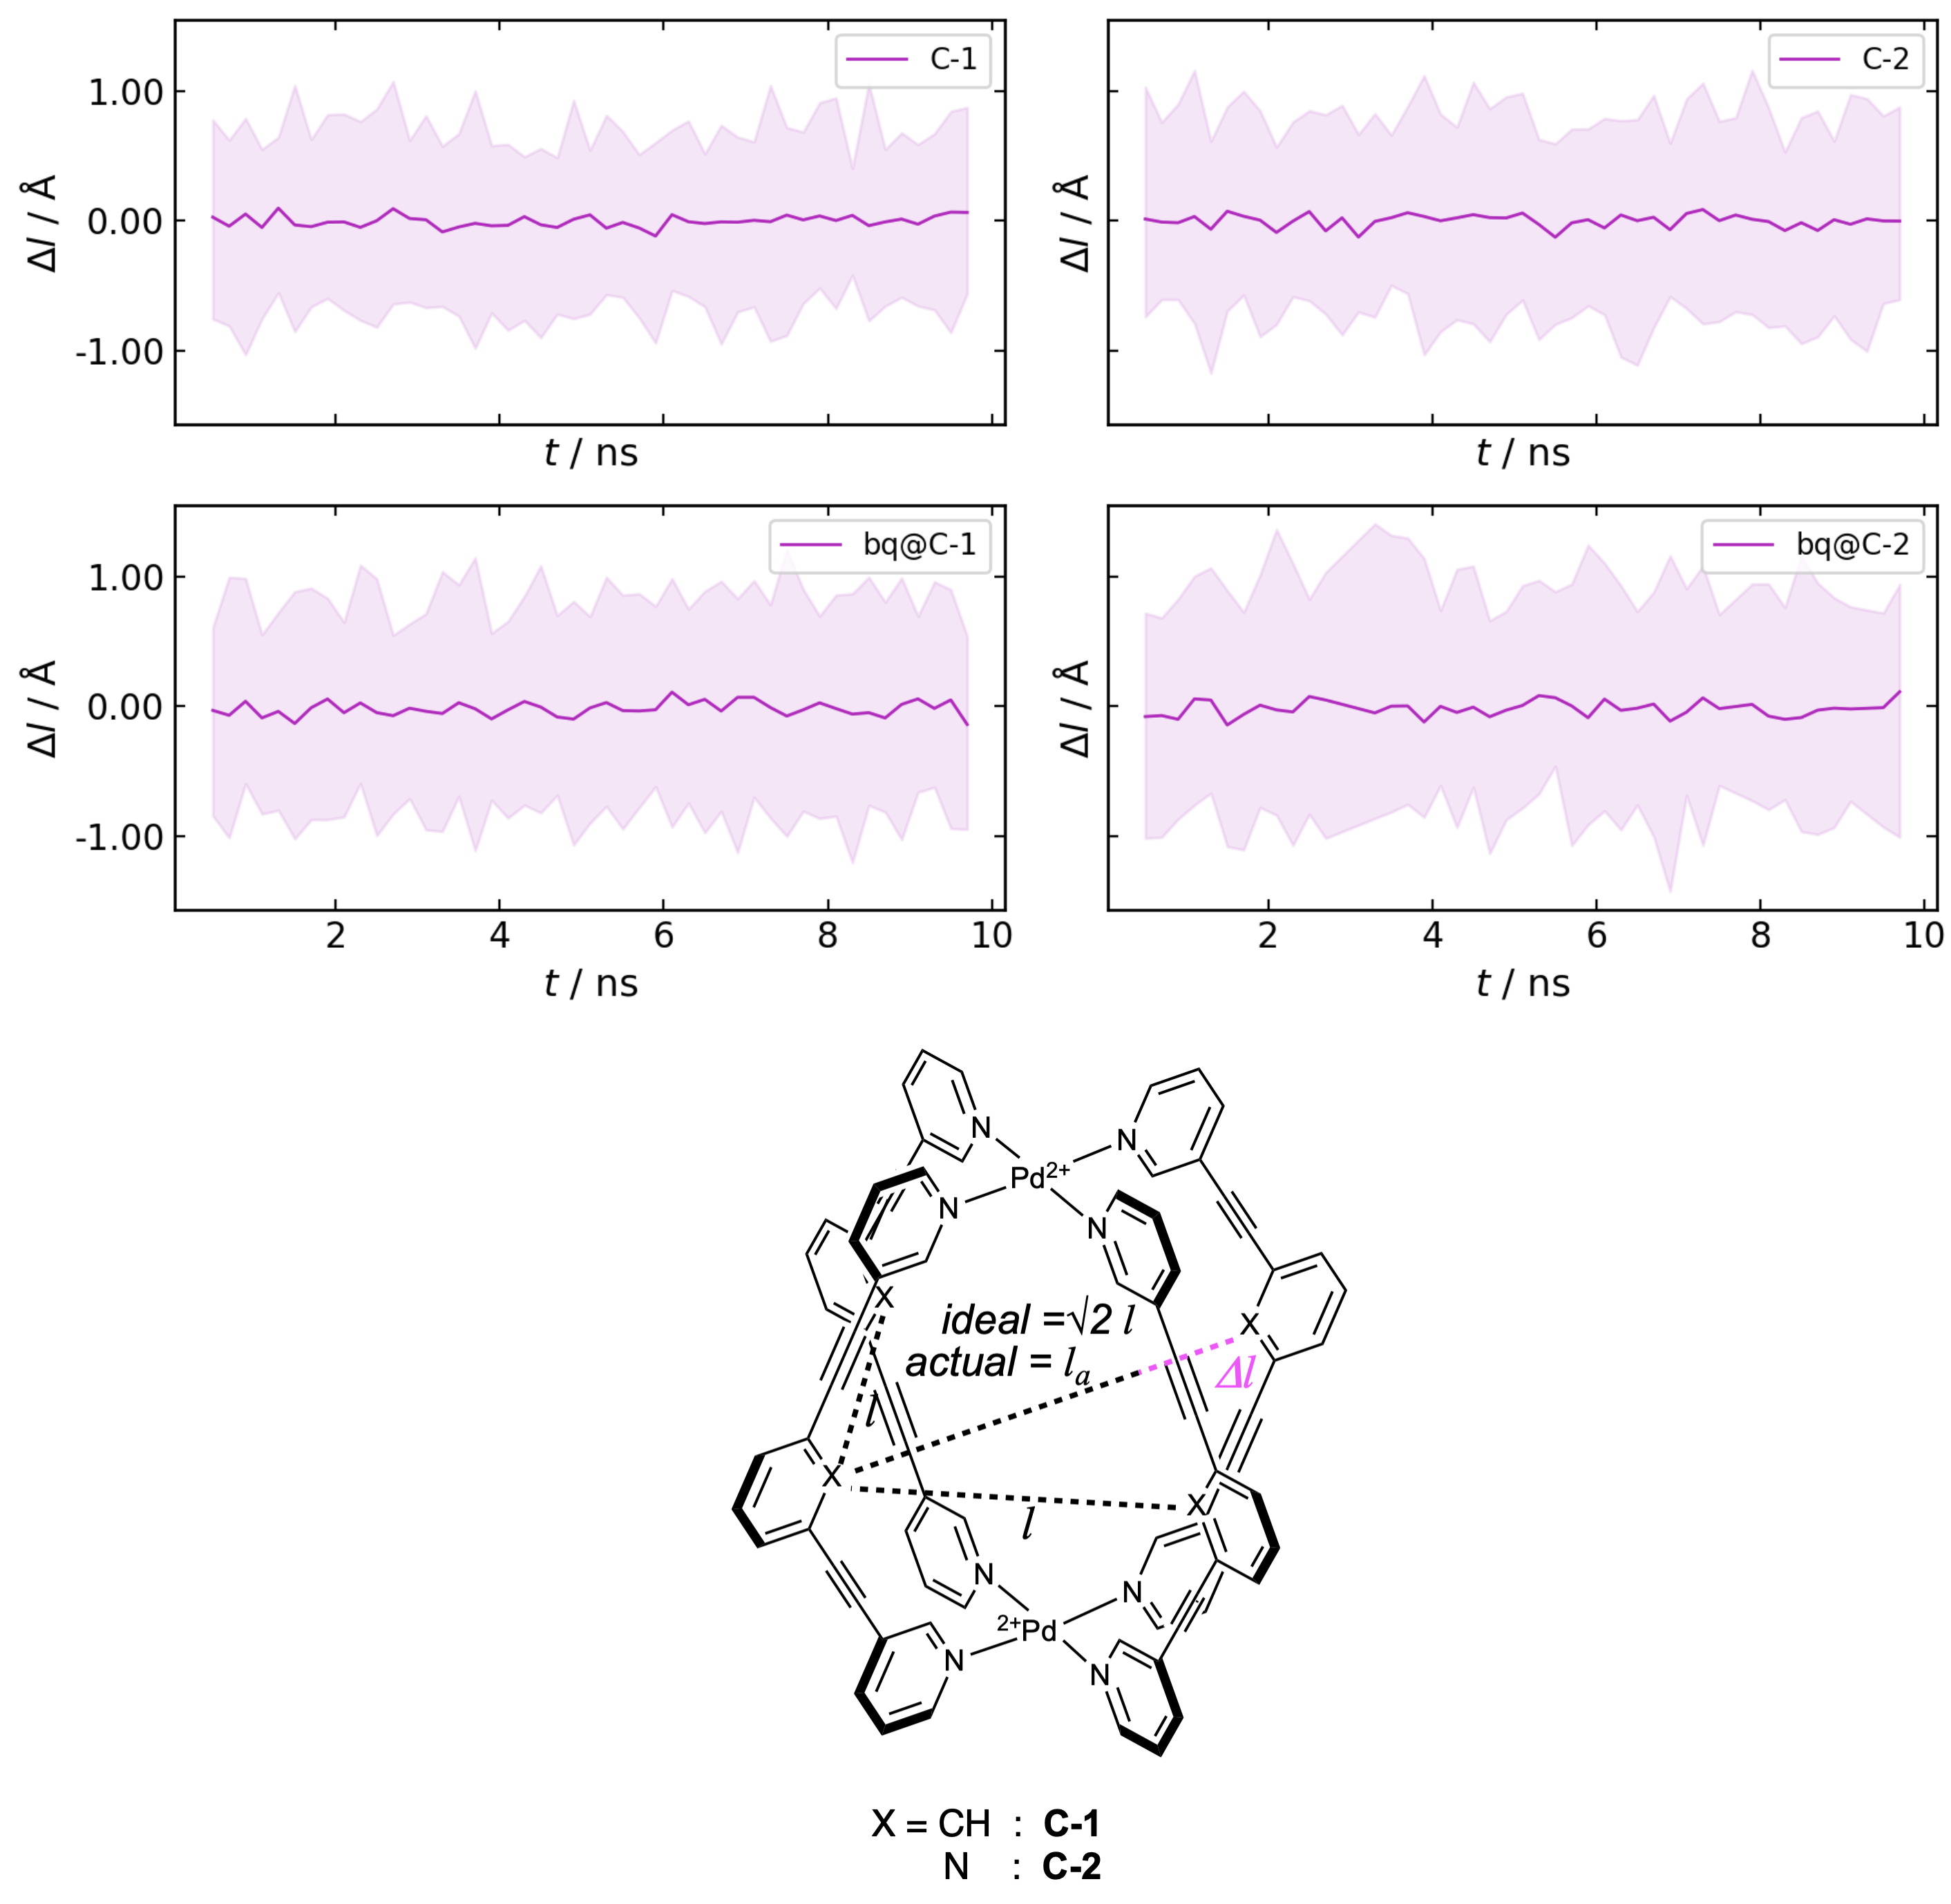
\includegraphics[width=\textwidth]{3/da//figs/figS5}
	\vspace{0.2cm}
	\hrule
	\caption{Temporal variation of the absolute value of $\Delta l$, a measure of squareness of the cavity.}
	\label{fig::si_da_5}
\end{figure}


\begin{figure}[h!]
	\vspace{0.4cm}
	\centering
	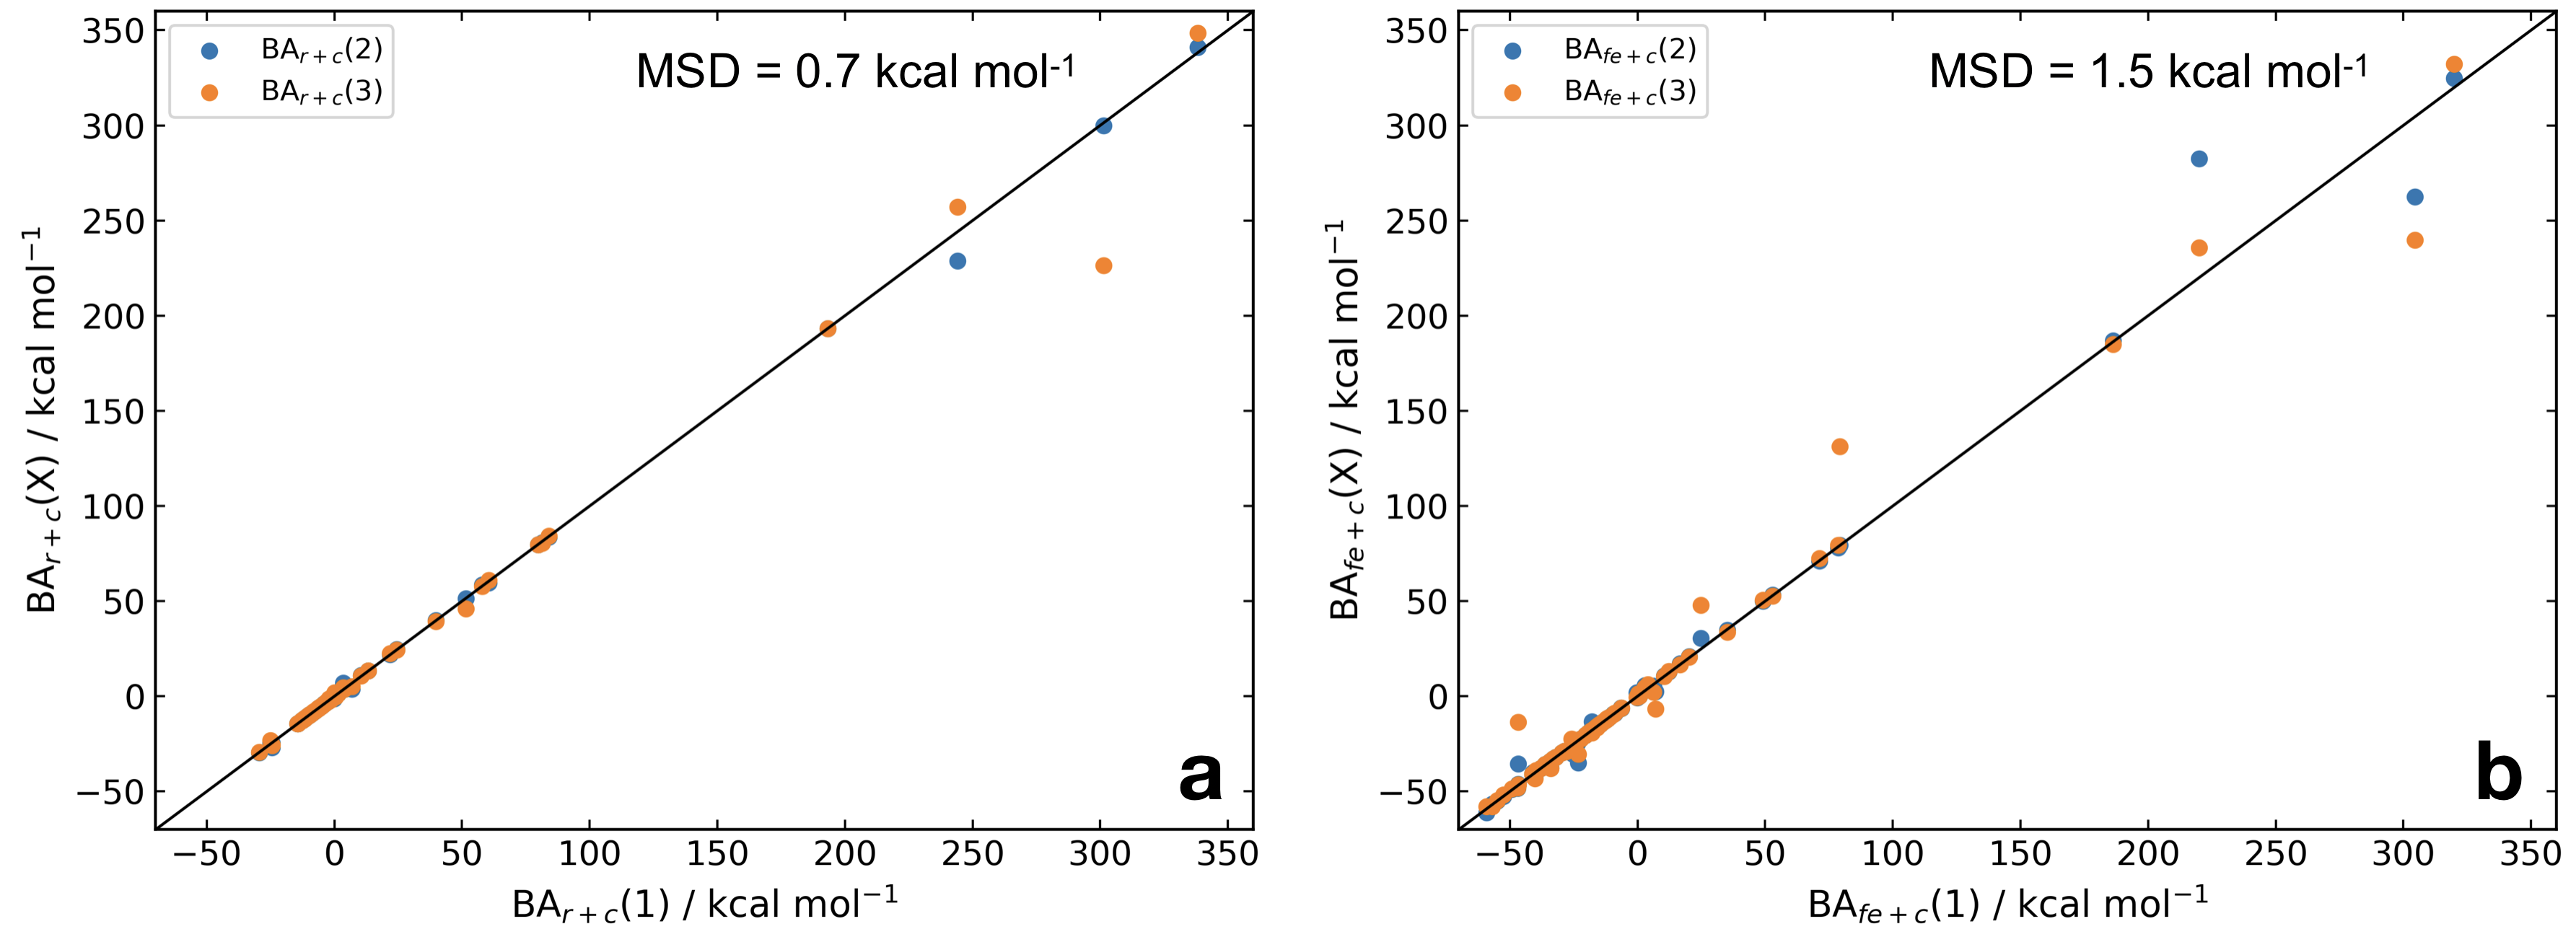
\includegraphics[width=\textwidth]{3/da//figs/figS6}
	\vspace{0.2cm}
	\hrule
	\caption{Temporal variation of the absolute deviation of $\theta$ from 90${}^\circ$.}
	\label{fig::si_da_6}
\end{figure}


\begin{figure}[h!]
	\vspace{0.4cm}
	\centering
	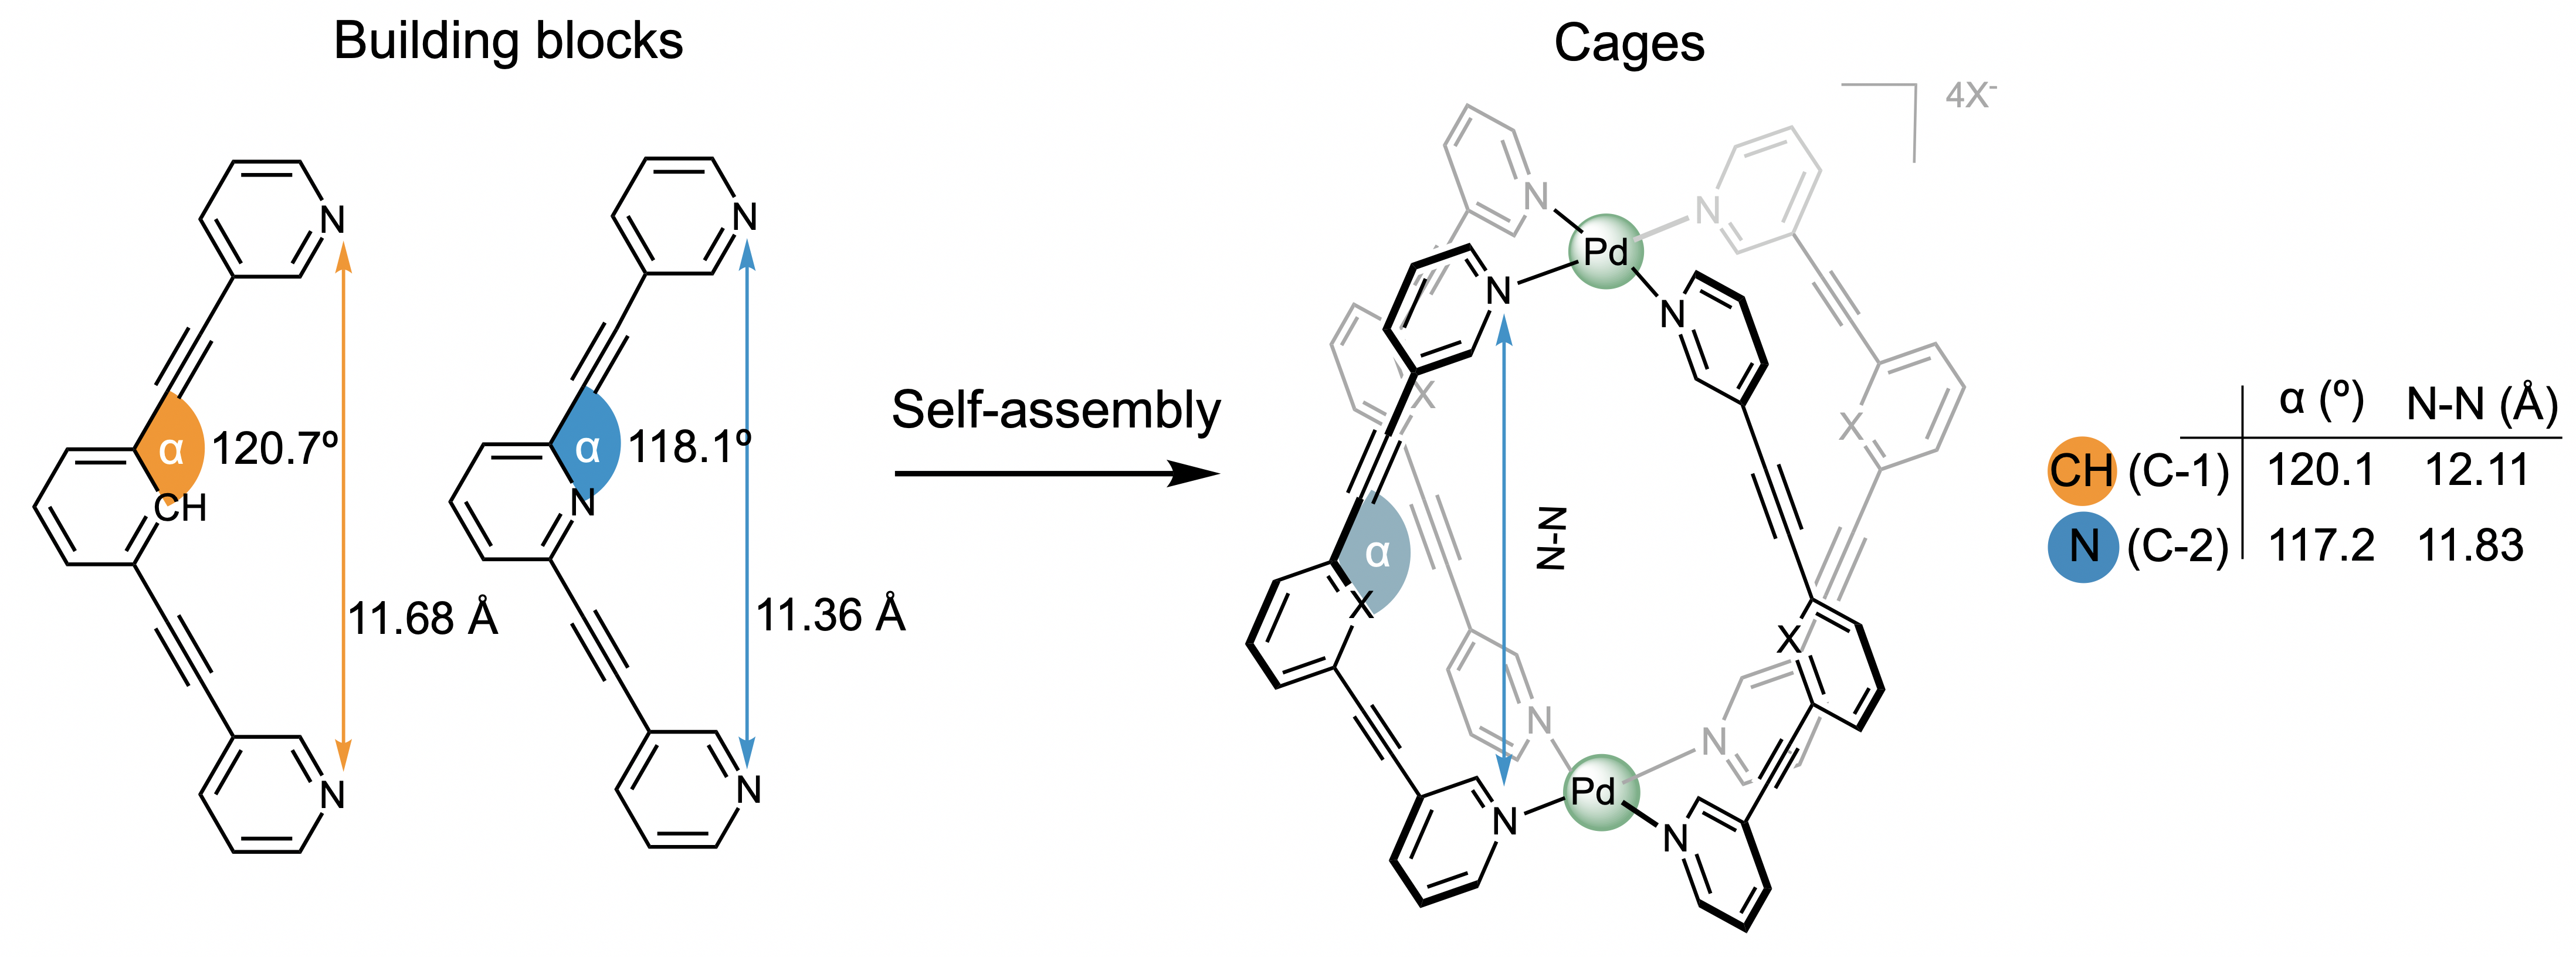
\includegraphics[width=\textwidth]{3/da//figs/figS7}
	\vspace{0.2cm}
	\hrule
	\caption{Illustration of the interior angles on the N-N distance in the D$_{4h}$-symmetric conformation.}
	\label{fig::si_da_7}
\end{figure}


\begin{figure}[h!]
	\vspace{0.4cm}
	\centering
	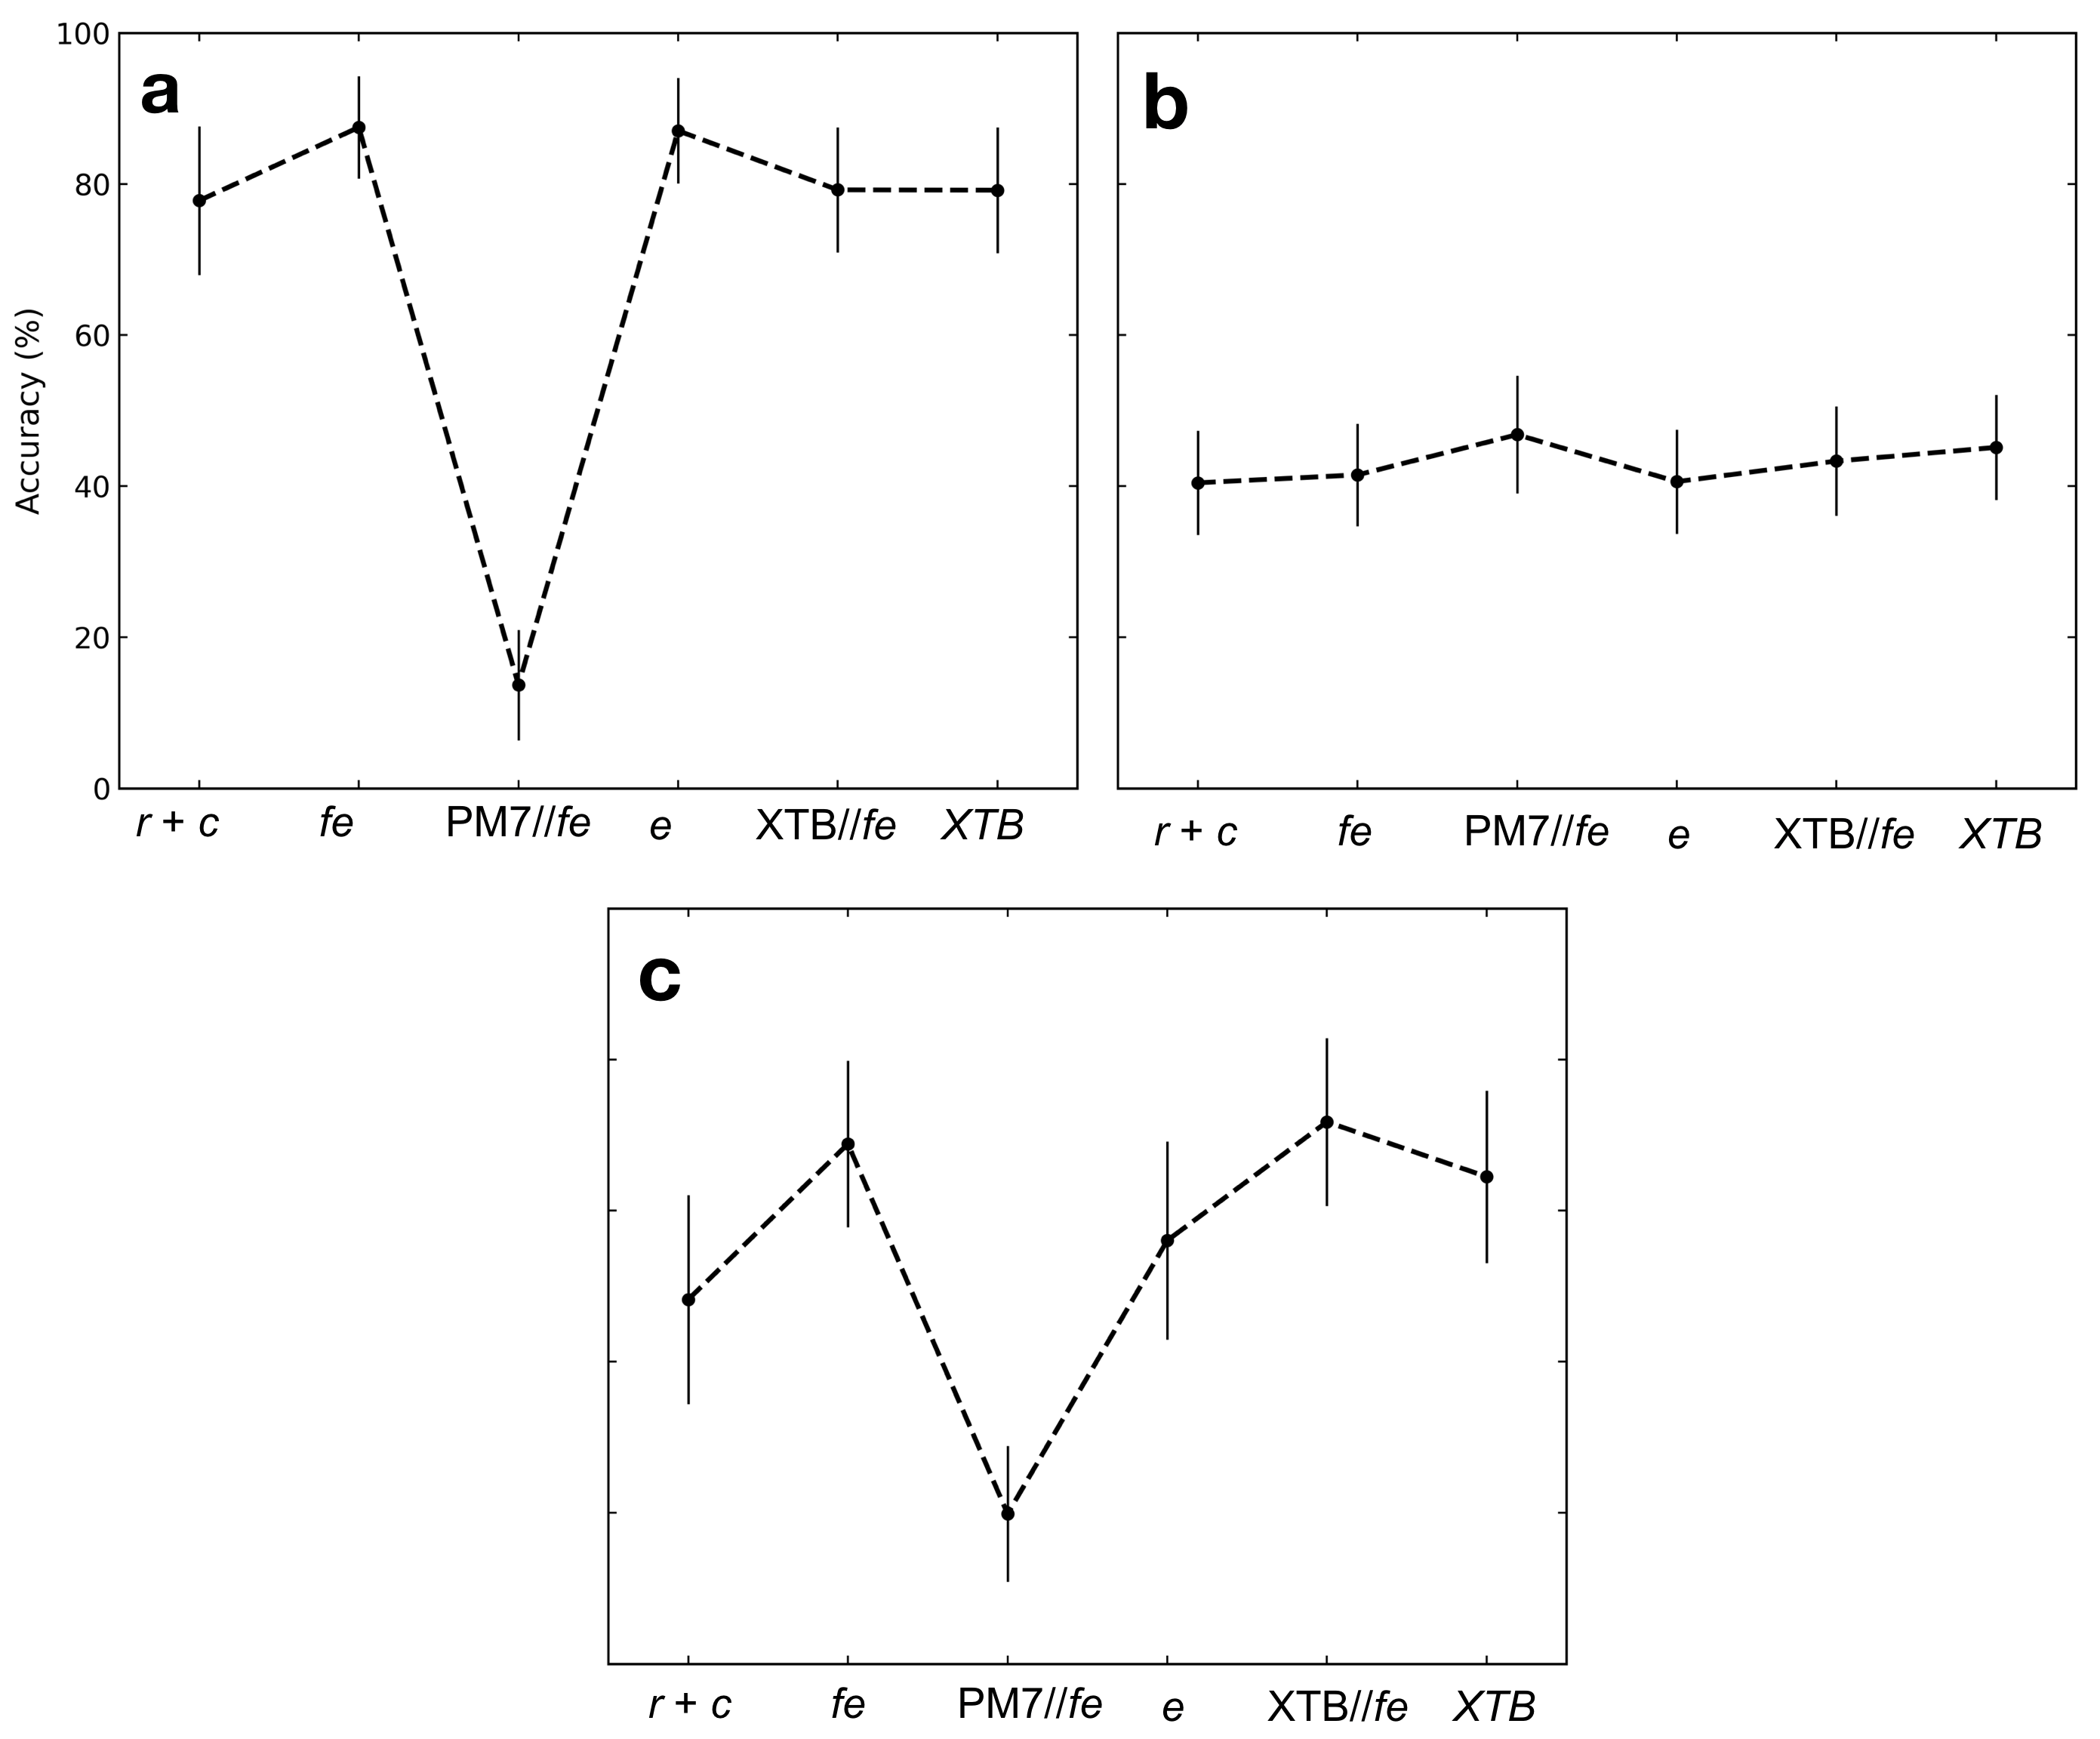
\includegraphics[width=\textwidth]{3/da//figs/figS8}
	\vspace{0.2cm}
	\hrule
	\caption{PES calculated at the M06-2X/def2-TZVP level of theory for rotation about the abcd dihedral for the linker in C-1 and C-2. This very small barrier is retained at a different level of DFT theory (PBE0-D3BJ/def2-TZVP) with $\Delta E^\ddagger$= 2.1, 1.3 \kcalx for L-1 and L-2 respectively. Note that these barriers are smaller than that for rotation of ethane ($\Delta E^\ddagger$ = 2.7 \kcalx calculated at the same M2 level, which compares well to the expt. \cite{Hirota1979} value of 2.9 \kcal).}
	\label{fig::si_da_8}
\end{figure}


\begin{sidewaystable}[h]
	\def\arraystretch{1.2}
	\begin{tabularx}{\textwidth}{YYYYYYYYYY}
		\hline
		Opt. Method & 	{\small{B3LYP/DZ}} &	{\small{PBE/DZ}}&	{\small{PBE-D3BJ/DZ}}	& {\small{PBE0/DZ}} & {\small{PBE0-D3BJ/DZ}} &	{\small{PBE-D3BJ/TZ}}	& {\small{PBE0-D3BJ/TZ}}	&
		{\small{M06-2X/TZ}} & {\small{M06-2X/TZ/
				SMD(DCM)}}
\\
		\hline

{\small{$\Delta E_\text{bind}$(bq$\subset$C-1)}}	&-19.7	&-23.0&	-35.2&	-27.1&	-22.7&	-35.5&	-29.4&	-25.4&	-5.5
\\
{\small{$\Delta E_\text{bind}$ (bq$\subset$C-2)}}	&-28.1&	-31.1&	-43.6&	-34.1&	-30.9	&-43.8&	-35.9&	-29.5&	-3.6
\\
{\small{$\Delta\Delta E_\text{bind}$(bq)}}&	-8.4&	-8.1&	-8.3&	-7.1	&-8.2&	-8.3&	-6.6&	-4.0&	2.0
\\
{\small{$\Delta E_\text{bind}$(aq$\subset$C-1)}}	&-20.4	&-26.4	&-52.4&	-43.8&	-26.7	&-53.8	&-47.1&	-40.2&	-16.8
\\
{\small{$\Delta E_\text{bind}$(aq$\subset$C-2)}}&	-21.5&	-27.3&	-52.6&	-43.5&	-26.9&	-53.4&	-45.6&	-35.2&	-13.1
\\
{\small{$\Delta\Delta E_\text{bind}$(aq)}}&	-1.1&	-0.9&	-0.3&	0.3&	-0.2&	0.4	&1.5&	5.1&	3.7
\\

\multicolumn{10}{c}{SMD(DCM)-M06-2X/def2-TZVP//Opt. Method}\\

{\small{$\Delta E_\text{bind}$(bq$\subset$C-1)}}&	-4.7&	-4.1&	-3.3&	-4.1	&-4.0&	-3.7&	-4.7&	-8.1&	-5.5a
\\
{\small{$\Delta E_\text{bind}$(bq$\subset$C-2)}}	&-5.7&	-4.9&	-4.3	&-5.3&	-3.3&	-4.4	&-4.9&	-3.8&	-3.6
\\
{\small{$\Delta\Delta E_\text{bind}$(bq)}}&	-1.0&	-0.8&	-1.1&	-1.2&	0.6&	-0.7&	-0.2&	4.2	& 1.9
\\
{\small{$\Delta E_\text{bind}$(aq$\subset$C-1)}}	&-8.6&	-8.7&	-10.3&	-10.1&	-9.5&	-9.3&	-11.9&	-14.2&	-16.8$^a$\\
{\small{$\Delta E_\text{bind}$(aq$\subset$C-2)}}	&-7.6&	-6.8&	-7.7&	-8.2&	-6.8&	-7.7&	-9.2&	-8.3&	-13.1
\\
{\small{$\Delta\Delta E_\text{bind}$(aq)}}&	1.0	&1.9&	2.6	&1.9&	2.8	&1.6&	2.7&	5.9	&3.7
\\

	\end{tabularx}
	\hrule
	\vspace{0.2cm}
	\caption{Effect of utilizing different optimization levels (MX) on $\Delta E_\text{bind}$  and  $\Delta\Delta E_\text{bind}$ (\kcal). All optimizations apart from PBE0-D3BJ/DZ were initialized from the PBE0-D3BJ/DZ-optimized geometries and single point energies calculated at SMD(DCM)-M06-2X/def2-TZVP where indicated. DZ = def2-SVP, TZ = def2-TZVP. $a.$ Optimization of C-1 required loose optimisation criteria and a quasi-Newton step method (rather than the default Rational function). }
	\label{table::si_da_3}
\end{sidewaystable}


\begin{figure}[h!]
	\vspace{0.4cm}
	\centering
	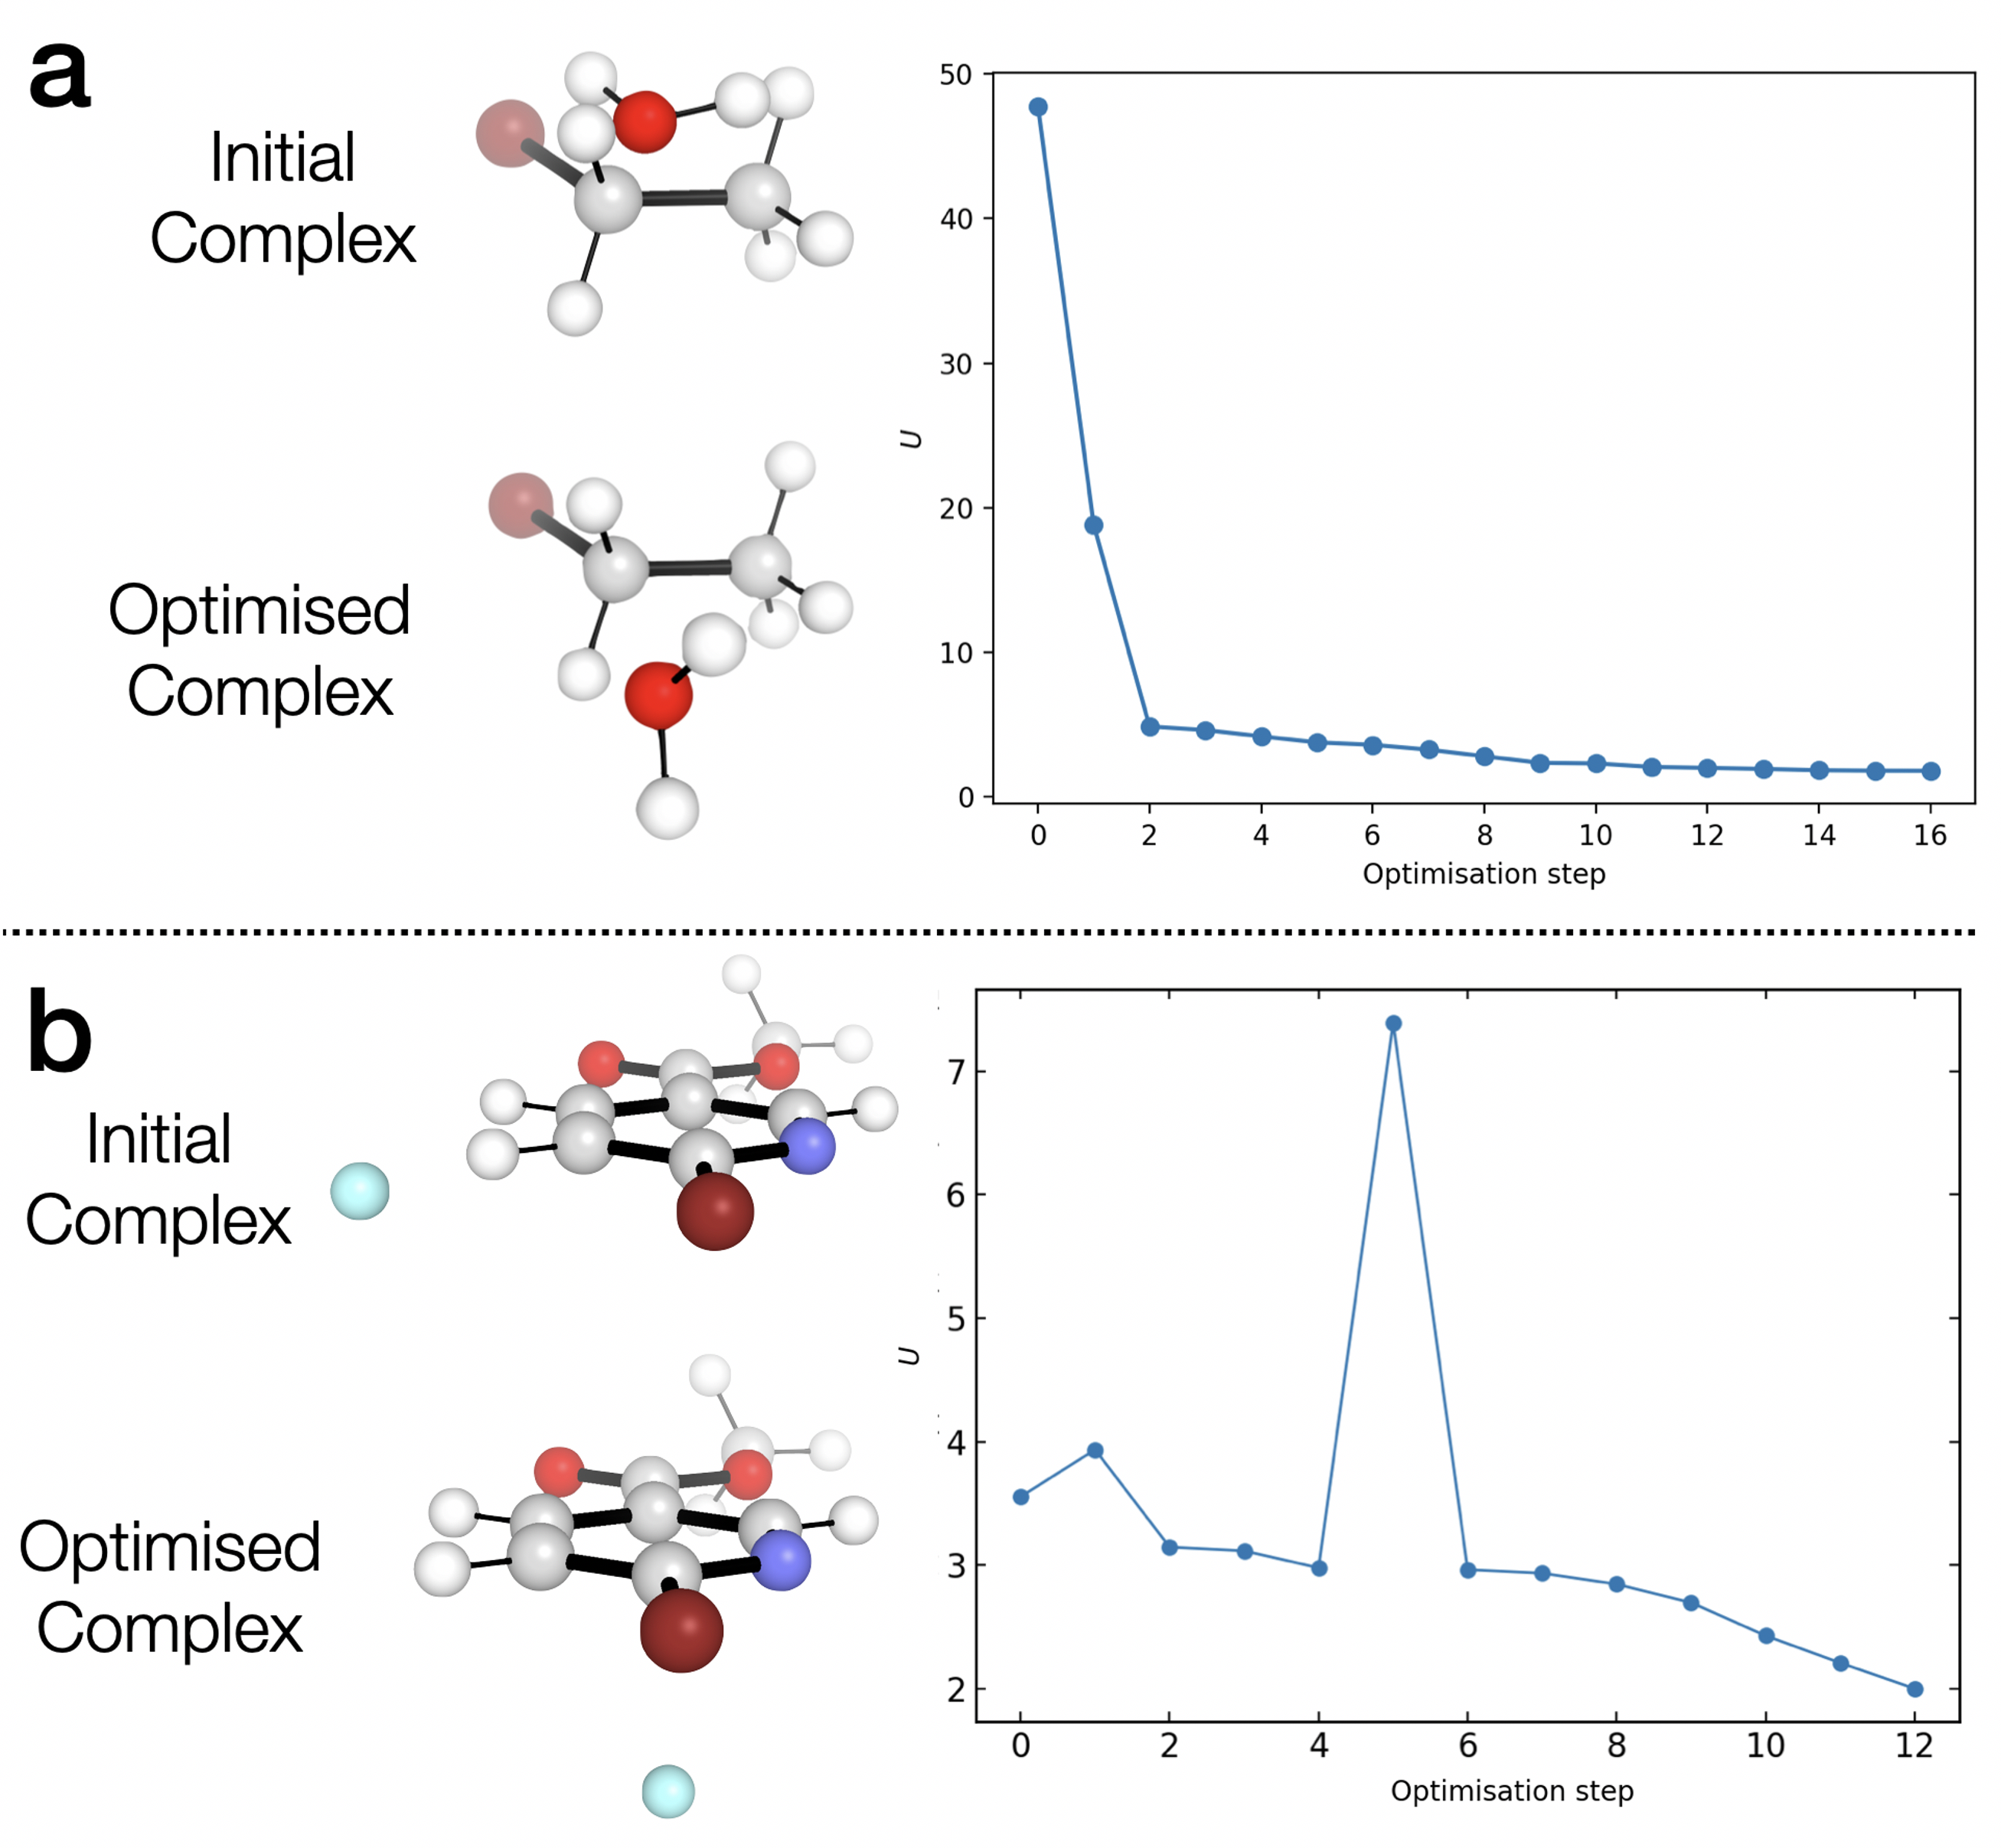
\includegraphics[width=13cm]{3/da//figs/figS9}
	\vspace{0.2cm}
	\hrule
	\caption{PM7 optimized geometries of cages and cage-substrate complexes.}
	\label{fig::si_da_9}
\end{figure}


\begin{figure}[h!]
	\vspace{0.4cm}
	\centering
	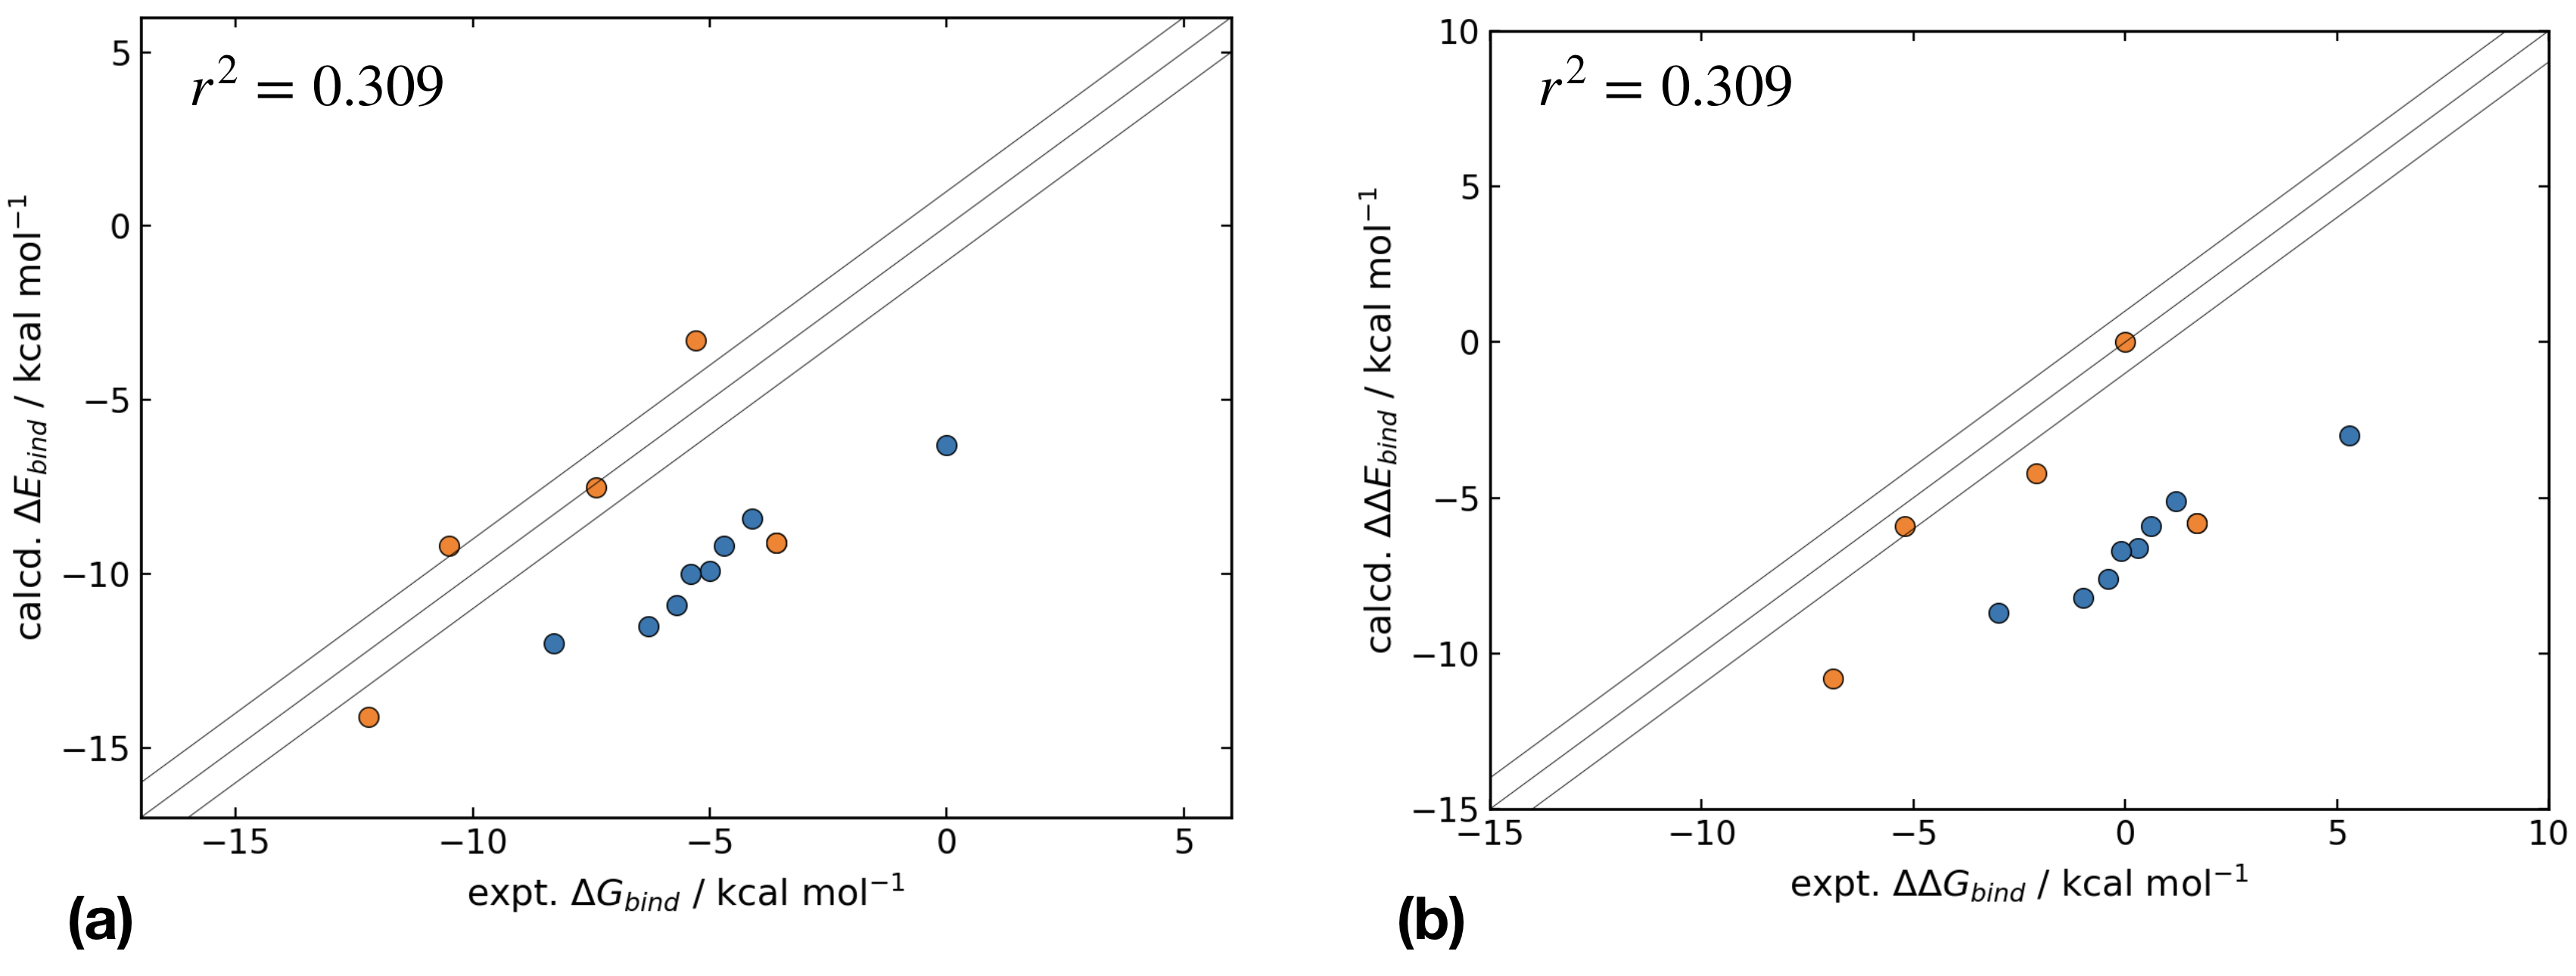
\includegraphics[width=\textwidth]{3/da//figs/figS10}
	\vspace{0.2cm}
	\hrule
	\caption{Correlation plots of (a) $\Delta E_\text{bind}$ and (b) $\Delta\Delta E_\text{bind}$ calculated at the PM7 level of theory. Orange and blue markers correspond to C-1 and C-2 cages, respectively. The different diagonals bracket the ±1 \kcalx area of accuracy.}
	\label{fig::si_da_10}
\end{figure}

\begin{figure}[h!]
	\vspace{0.4cm}
	\centering
	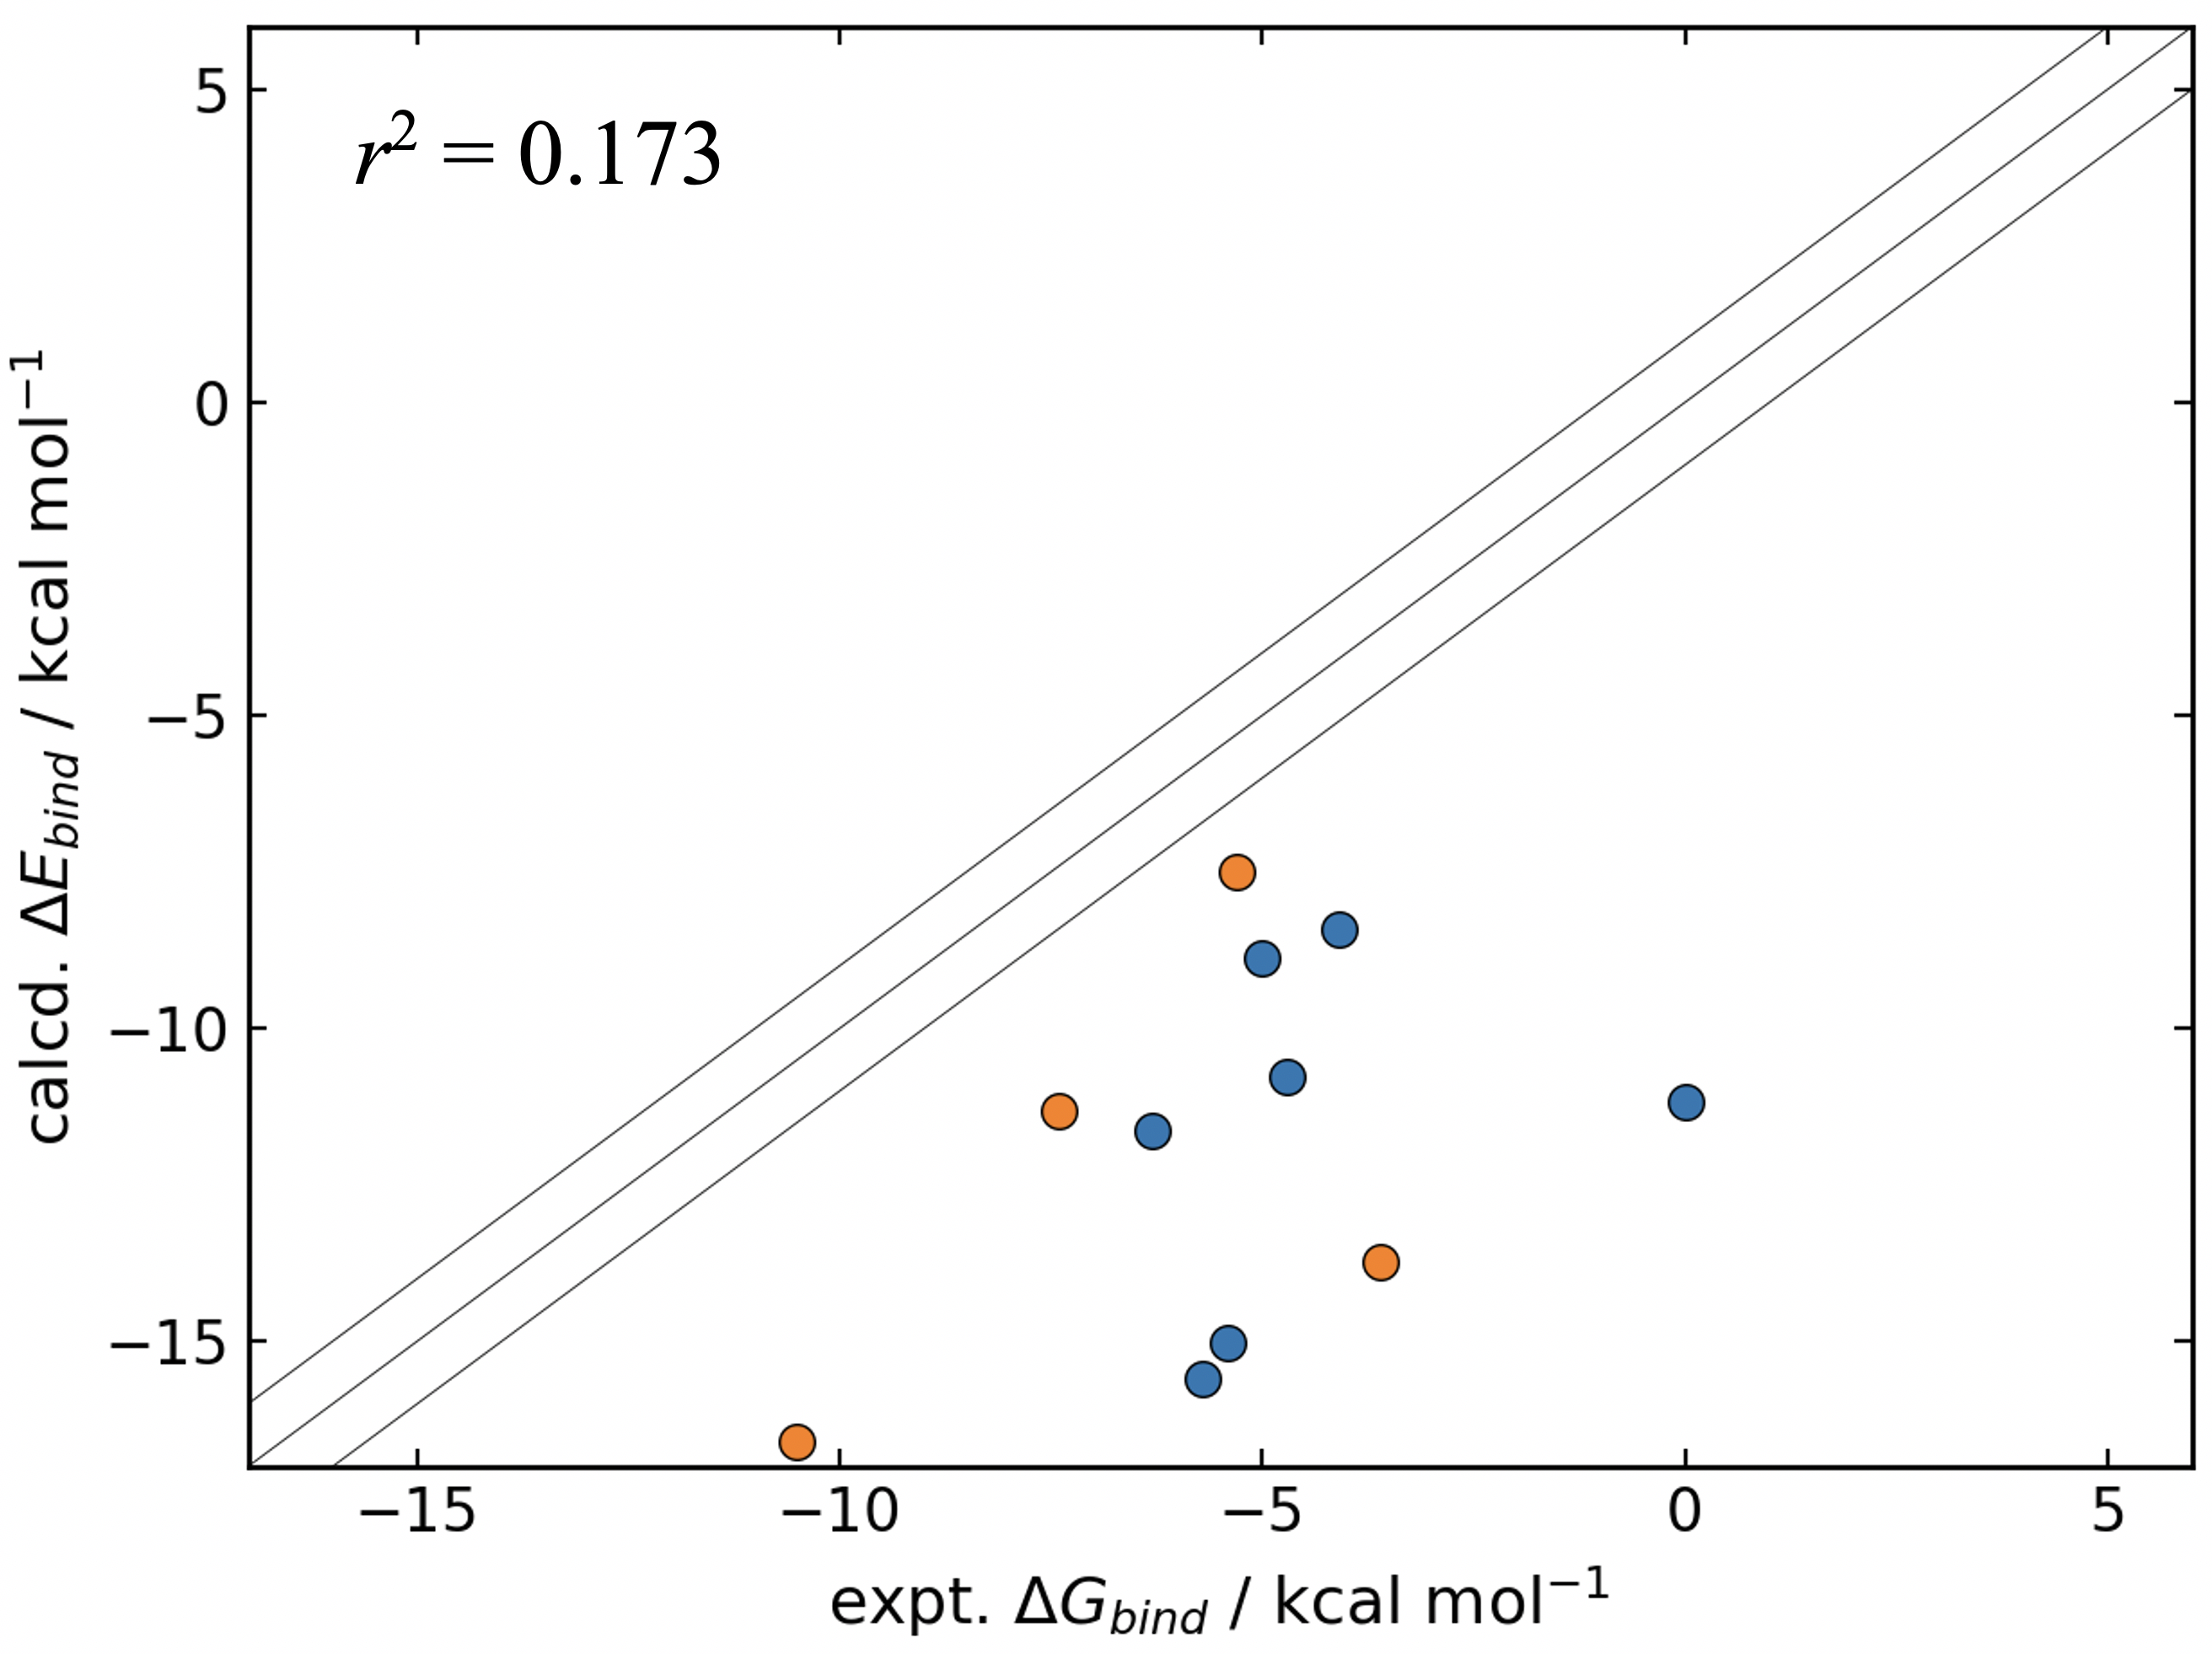
\includegraphics[width=9cm]{3/da//figs/figS11}
	\vspace{0.2cm}
	\hrule
	\caption{Correlation plots of $\Delta E_\text{bind}$ calculated at the SMD(DCM)-M06-2X/def2-TZVP//tight-binding DFT (GFN-xTB) level of theory. Orange and blue markers correspond to C-1 and C-2 cages, respectively. The different diagonals bracket the ±1 \kcalx area of accuracy.}
	\label{fig::si_da_11}
\end{figure}

\clearpage  % <- don't delete me
\subsection{Thermodynamic Contributions}
\label{section::da_si_3_3}

While thermodynamic contributions are required to obtain binding free energies ($\Delta G_\text{bind}$) and to compare to experiments directly, the accurate quantification remains challenging. Furthermore, the accuracy (in principle) gained by including these contributions comes with a much higher computational cost. For large systems, as the one considered here, the computational cost increase is from a few hours to a couple of days.\footnote{For example, the analytical hessian required to compute the vibrational frequencies for the zero-point energy and vibrational entropy components for bq$\subset$C-1 took 808 CPUh (M1) while the optimisation (M1) and single point (SMD(DCM)-M2) calculation took 36 CPUh.}

The free energy of binding qn in C-X is given by,

\begin{equation}
	\Delta G_\text{bind}(\text{qn}\subset\text{C-X}) =\Delta E_\text{bind} (\text{qn}\subset\text{C-X})+\Delta G_\text{cont}(\text{qn}\subset\text{C-X})
		\label{dg_bind}
	\end{equation}
	
and the relative free energy of binding qn is defined in,
\begin{equation}
	\begin{aligned}
		\Delta\Delta G_\text{bind} &= [\Delta E_\text{bind} (\text{qn}\subset\text{C-2}) + \Delta G_\text{cont} (\text{qn}\subset\text{C-2})] - [\Delta E_\text{bind} (\text{qn}\subset\text{C-1})  + \Delta G_\text{cont} (\text{qn}\subset\text{C-1})] \\
		&= \Delta\Delta E_\text{bind}  + \Delta\Delta G_\text{cont}
	\end{aligned}	
\end{equation}


Where $\Delta G_\text{cont}$ are the thermodynamic corrections to the potential energy difference ($\Delta E_\text{bind}$) given by the inverse of \eqref{dg_bind}.

These corrections include an enthalpic contribution ($H_\text{cont}$) containing the zero-point energy (ZPE), thermal energy plus $k_BT$, and an entropic contribution ($TS_\text{cont}$), which contains contributions from translation, rotation, vibration and electronic degrees of freedom. Table \ref{table::si_da_5} outlines these components retrieved directly from frequency calculations from the ORCA package for C-1/C-2, bq and bq$\subset$C-1/bq$\subset$C-2. Note that the electronic entropy is zero.

As can be seen in Table \ref{table::si_da_5}, the thermodynamic contributions to the binding energy ($\Delta G_\text{cont}$) of bq in C-1 and C-2 are large in magnitude but very similar ($\Delta G_\text{cont}$(bq$\subset$C-1) = 14.9 \kcal, $\Delta G_\text{cont}$(bq$\subset$C-2) = 16.0 \kcal) due to the almost identical enthalpic and entropic contributions. This explains why the calculated relative binding affinities ($\Delta\Delta E_\text{bind}$) closely match the experimental binding free energies (i.e. $\Delta\Delta E_\text{bind} \sim \Delta\Delta G_\text{bind}$). Secondly, the large positive free energy contribution ($\Delta G_\text{cont}$) to the binding energy for both C-1 and C-2 would suggest a very unfavourable binding process (i.e.$\Delta G_\text{bind}$(bq$\subset$C-1) and $\Delta G_\text{bind}$(bq$\subset$C-2) $> 0$), which is contrary to experimental observations. These results give rise to two possibilities, either (1) $\Delta G_\text{cont}$ is incorrect (mostly due to entropic contributions) or (2) $\Delta E_\text{bind}$ is underestimated when calculated using the SMD(DCM)-M06-2X/def2-TZVP methodology. The following sections explain how the former, given the literature available, is the most plausible scenario.


\begin{table}[h]
	\def\arraystretch{1.7}
	\begin{tabularx}{\textwidth}{YYYYYYY}
		\hline
		&$H_\text{cont}$&	$TS_\text{trans}$	&$TS_\text{rot}	$&$TS_\text{vib}$&	$TS_\text{tot}$&$G_\text{cont}$ 
\\
		\hline
		
		C-1	&712.0	&14.1&	12.8&	79.6&	106.6&	605.5
\\
		bq$\subset$C-1	&773.1&	14.2&	12.9&	90.7	&117.8&	655.3
\\
		C-2	&681.6	&14.1	&12.8&	79.1&	106.0&	575.6
\\
		bq$\subset$C-2	&742.9&	14.2&	12.8&	89.4&	116.5&	626.4
\\
		bq&	58.4&	11.9&	8.3	&3.4&	23.5	&34.8
\\
		$\Delta$(bq$\subset$C-1)&	2.6	&-11.8&	-8.3&	7.8&	-12.3&	14.9
\\
		$\Delta$(bq$\subset$C-2)&	2.8	&-11.8&	-8.3&	7.0	&-13.1&	16.0
\\
		&$\Delta\Delta H_\text{cont}$&	$T\Delta\Delta S_\text{trans}$	&$T\Delta\Delta S_{rot}$&	$T\Delta\Delta S_\text{vib}$&	$T\Delta\Delta S_\text{tot}$&	$\Delta\Delta G_{cont}$ 
\\
     	&	-0.2&	0.0	&0.0&	0.8	&0.8 &	-1.0
\\
		
	\end{tabularx}
	\hrule
	\vspace{0.2cm}
	\caption{Thermodynamic contributions (\kcal) to the potential energy calculated at the PBE0-D3BJ/def2-SVP level of theory obtained directly from ORCA. $\Delta X_\text{bind}$ = bq$\subset$C-X – (bq + C-X); X=$H, S, G$.}
	\label{table::si_da_5}
\end{table}


To do so, we analysed the entropic components ($T\Delta S_\text{total}$), which is the dominant contrition to $\Delta G_\text{cont}$). The partition function used to calculate the translational entropy derives from a particle in a box (PIB) treatment of the potential, within an ideal gas model of the system. In this scenario, at standard-state, the effective volume of a molecule is $V = RT/p \; (p = 1$ atm), which is an overestimation of the ‘real’ volume available, and therefore an overestimation of the translational entropy upon binding. A more appropriate effective volume can be obtained by moving to a 1 M ‘standard state’,\cite{Ribeiro2011} which when calculated with $TS_{1 atm \rightarrow 1 M} = RT \ln(c^\standardstate_\text{1 atm} / c^\standardstate_\text{1 M})$ leads to a contribution of 1.9 \kcalx at 298 K for each species considered.

This correction reduces the translational entropy term; for a two to one change in molecularity (e.g. A+B $\rightarrow$ C) this reduction is 1.9 \kcal. Using this correction, $\Delta G_\text{cont}$(bq$\subset$C-1) = 13.1 \kcalx and $\Delta G_\text{cont}$(bq$\subset$C-2) = 14.1 \kcalx (Table \ref{table::si_da_6}).


\begin{table}[h]
	\def\arraystretch{1.7}
	\begin{tabularx}{\textwidth}{YYYYY}
		\hline
		&1 atm, qRRHO &	1 M, qRRHO&	1 M, HO&	1 M, HO, real freqs 
\\
		\hline
		
		{\small{$\Delta G_\text{cont}$(bq$\subset$C-1)}}&	14.9	&13.0&	1.2	&11.6
\\
		{\small{$\Delta G_\text{cont}$(bq$\subset$C-2)}}	&16.0&	14.1&	12.5&	12.3
\\
		
	\end{tabularx}
	\hrule
	\vspace{0.2cm}
	\caption{Free energy contributions (\kcal) calculated at the PBE0-D3BJ/def2-SVP level of theory using different treatments of the translational entropy and low frequency modes.}
	\label{table::si_da_6}
\end{table}

However, despite this correction, there is still an inconsistency in the treatment of the translational entropy. In solution the translation of bq and C-1 are treated as a particle in a box, while within C-1, the translation of bq is treated by an interpolation of a harmonic oscillator (HO) and rigid rotor (RR), this quasi-RRHO approximation is the default in the ORCA package. While Grimme’s quasi-RRHO approximation\cite{Grimme2012} is suitable for treating low-frequency normal modes corresponding to rotations, obviously it is inappropriate for treating a translational mode such as those depicted in Figure \ref{fig::si_da_12}, which are treated as $>$90\% free rotors within the default weighting scheme used by Grimme and implemented in ORCA (Figure \ref{fig::si_da_13}). 

Treating all the modes harmonically partially removes the dampening of the low frequency modes contribution to the entropy and again reduces $\Delta G_\text{cont}$. Using the harmonic approximation along with the 1 M standard stare correction within our otherm code \\ (\url{https://github.com/duartegroup/otherm}) we obtain $\Delta G_\text{cont}$(bq$\subset$C-1) = 11.2 \kcal and $\Delta G_\text{cont}$(bq$\subset$C-1) = 12.5 \kcalx (Table  \ref{table::si_da_6}). Of course, this then removes the more correct treatment of modes which correspond to rotations.


\begin{figure}[h!]
	\vspace{0.4cm}
	\centering
	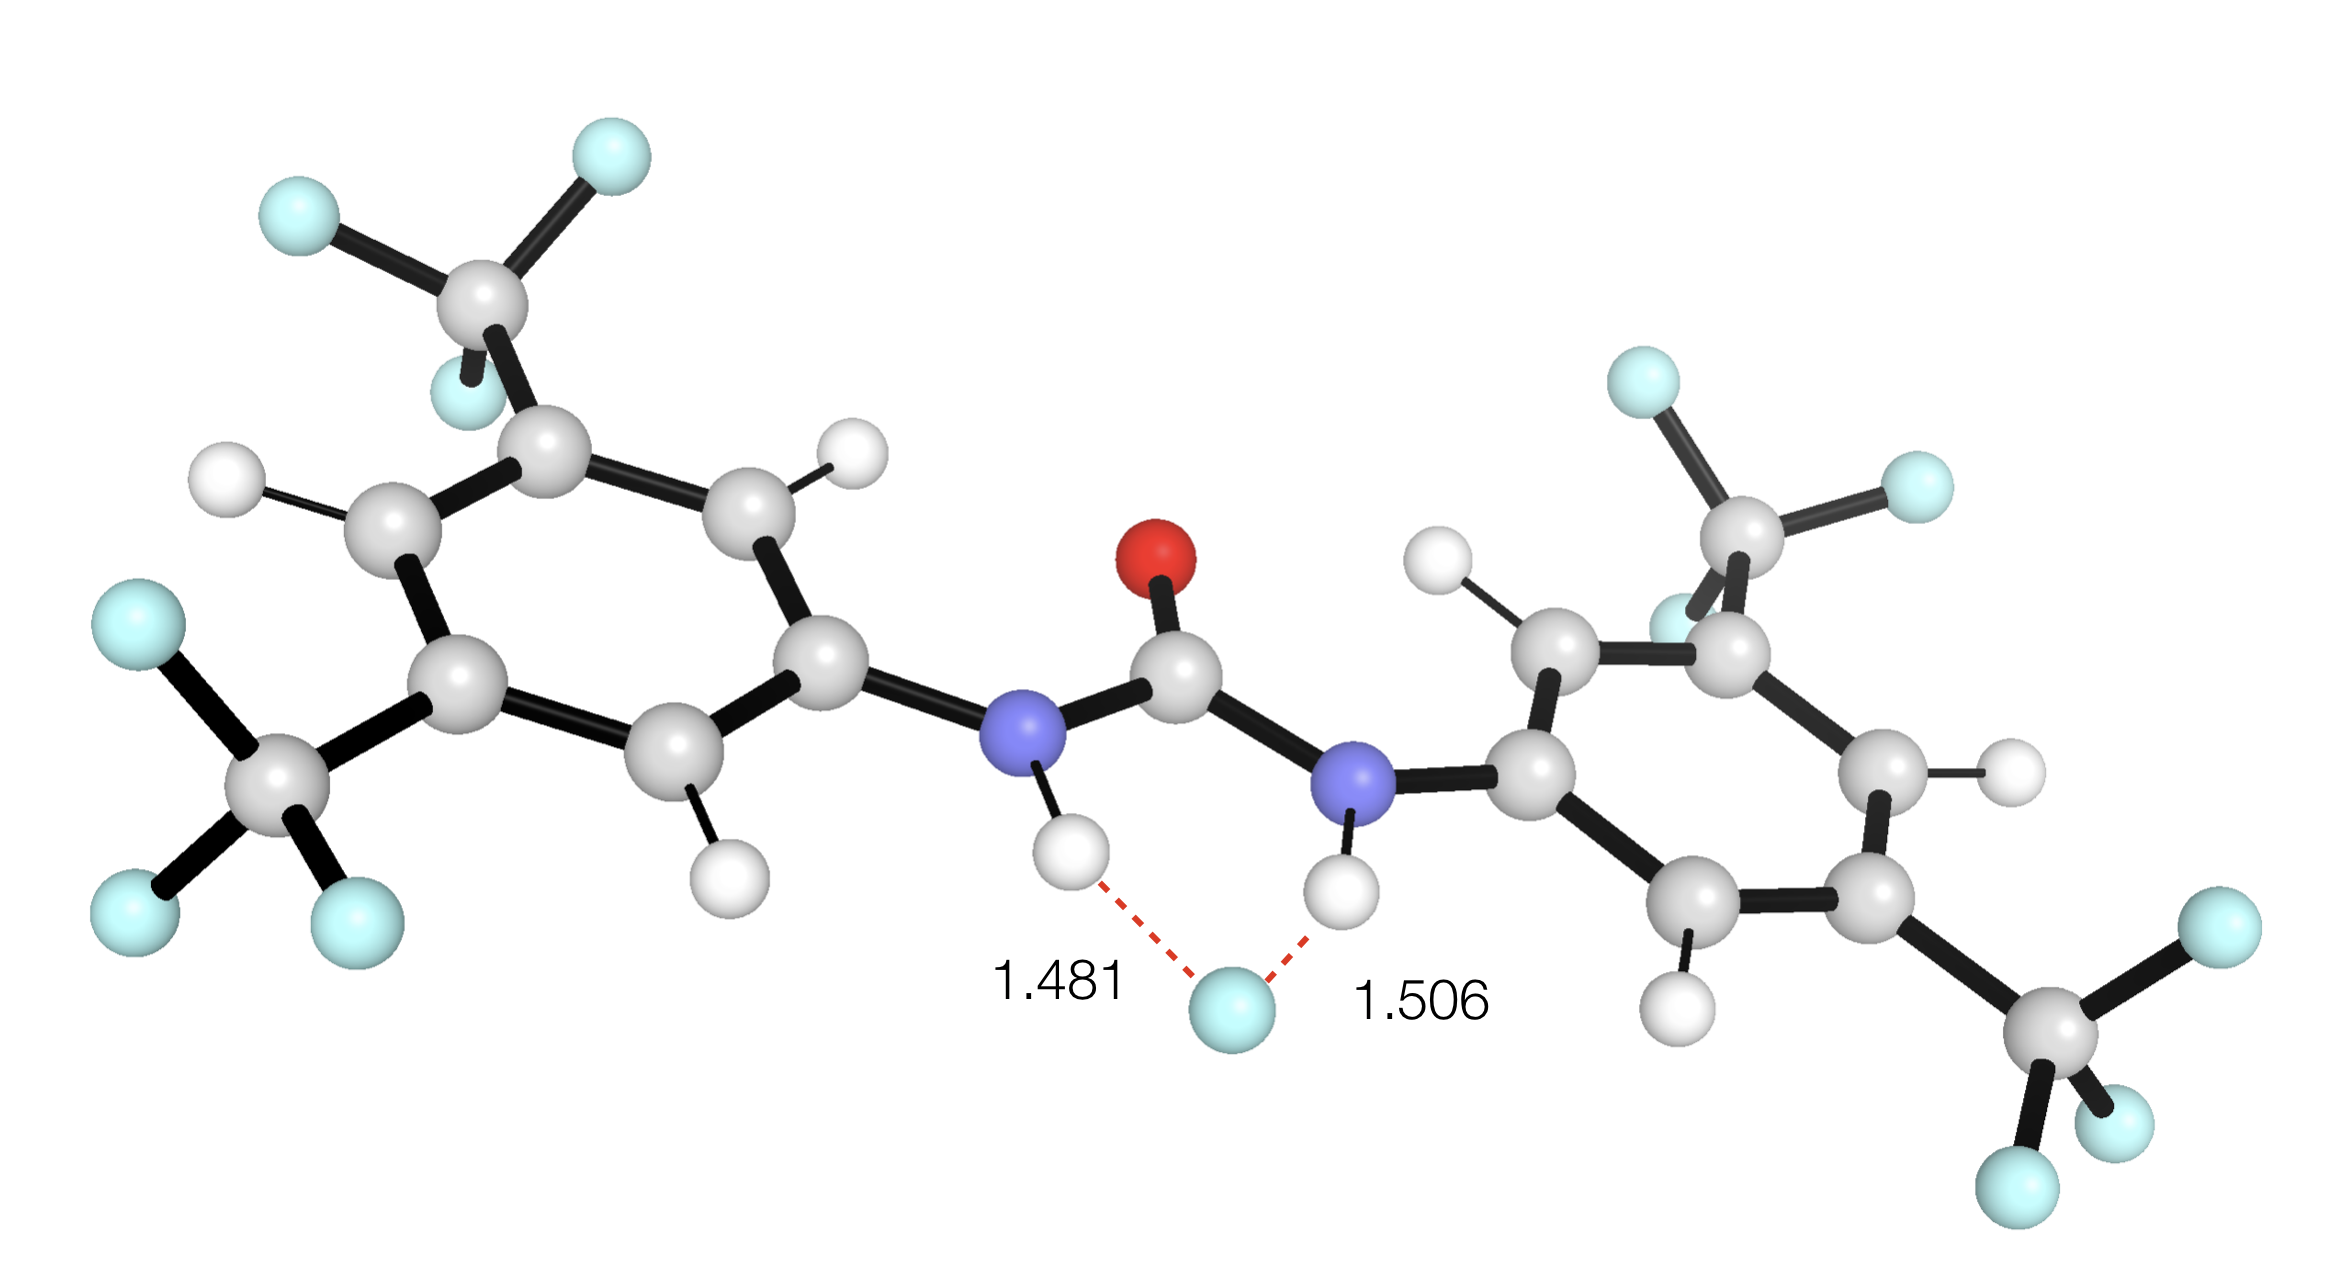
\includegraphics[width=\textwidth]{3/da//figs/figS12}
	\vspace{0.2cm}
	\hrule
	\caption{Normal modes of bq in C-1 dominated by $x, y, z$ translation calculated at M1 annotated with scaled displacement vectors calculated in Chemcraft v. 1.8.}
	\label{fig::si_da_12}
\end{figure}

\begin{figure}[h!]
	\vspace{0.4cm}
	\centering
	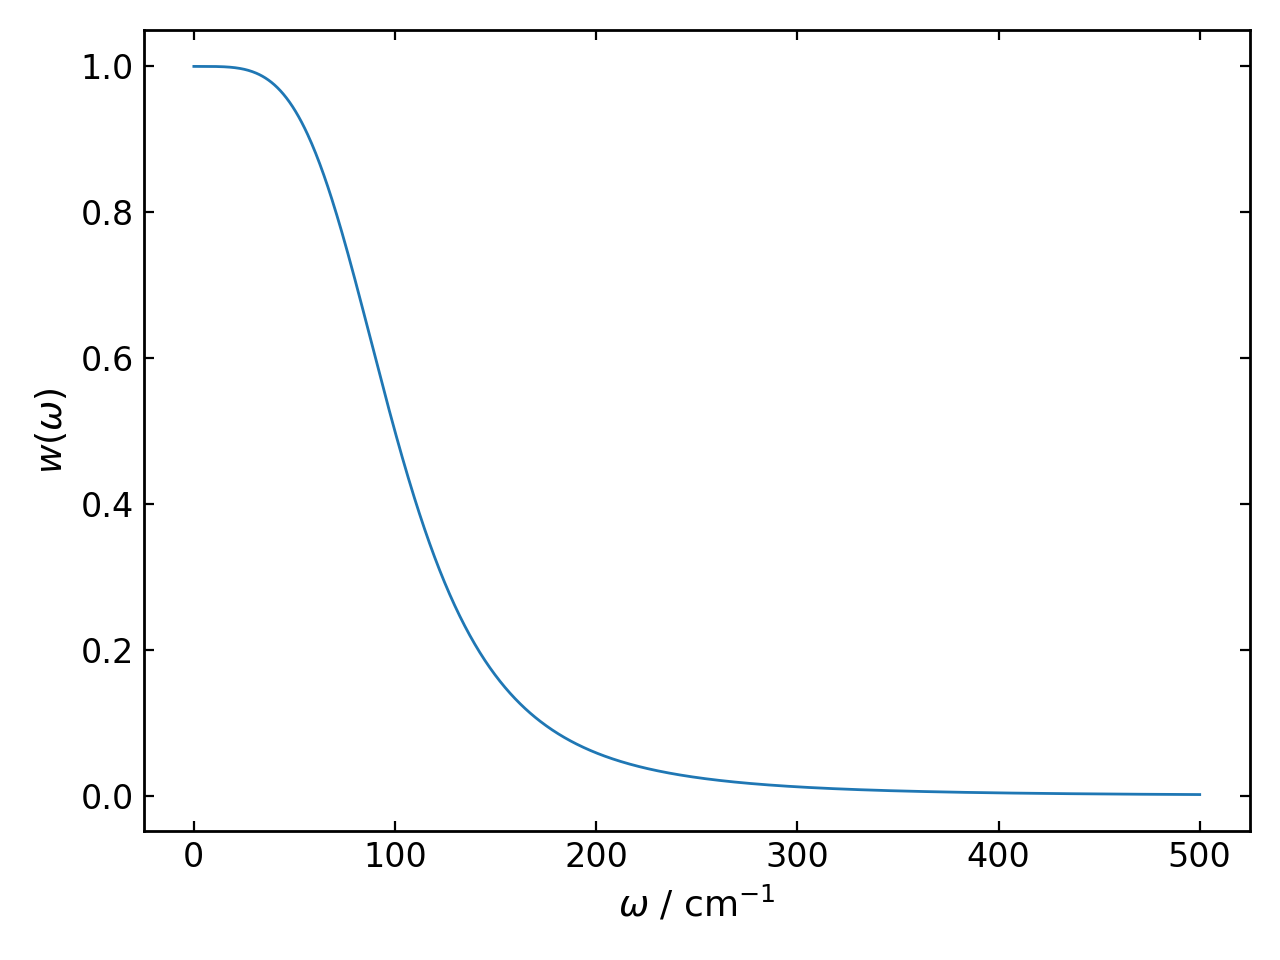
\includegraphics[width=9cm]{3/da//figs/figS13}
	\vspace{0.2cm}
	\hrule
	\caption{Weighting utilized within the q-RRHO approximation to interpolate between the free rotor and harmonic oscillator expressions of the entropy as a function of normal mode frequency ($\omega$).}
	\label{fig::si_da_13}
\end{figure}


Furthermore, we note that with the exception of bq both cages and cage-substrate complexes contain small imaginary modes (all $< 20$i cm$^{-1}$) due to one or more of (1) premature geometry convergence, (2) numerical errors in the Hessian, (3) the resolution of identity (RIJCOSX) approximation or (4) convergence to a saddle point. This observation is common in large supramolecular structures,\cite{Daver2017} and poses another issue when calculating the vibrational contribution to the free energy (both entropic and enthalpic). Harvey et al. proposed treating these modes as real rather than discarding them as both ORCA and Gaussian do by default. Doing so we have $\Delta G_\text{cont}$(bq$\subset$C-1) = 11.6 \kcalx and $\Delta G_\text{cont}$(bq$\subset$C-1) = 12.3 \kcalx (Table \ref{table::si_da_6}). These differences are still very similar to the treatment without these modes, due to their being a fortuitous cancellation between the reactant (C-1 + bq, C-2 + bq) and product (bq$\subset$C-1, bq$\subset$C-2) as both C-1 and bq$\subset$C-1 possessed two imaginary frequencies and C-2 and bq$\subset$C-2 both contained a single imaginary frequency.

These results show that, despite moving from an almost entirely RR approximation to the HO approximation for the low frequency modes and treating the imaginary modes as real, the difference in free energy contribution on binding is still large and positive ($\sim$ 10 \kcal). New methods have been recently developed to improve the estimation of the effective volume based on the HO approximation.\cite{Tarumi2018, Nakai2014}

Finally, we note that from the molecular dynamics calculations the cavity is not empty prior to substrate binding, containing in average one solvent molecule in the cavity (Figure \ref{fig::si_da_14}). Himo and Harvey have previously shown that consideration of solvent occupying the internal volume of supramolecular systems is important to reach quantitative results.\cite{Daver2017} In fact, considering the cage to be occupied by a single DCM solvent molecule, the binding process can be represented as:
DCM$\subset$C-X + qn $\rightarrow$ qn$\subset$C-X + DCM
In this case the translational entropy component of the free energy change quenches dramatically ($T\Delta S_\text{trans}$(bq$\subset$C-1)$ = -0.2$ \kcal, Table \ref{table::si_da_7}). This in turn has the effect of reducing the free energy contribution difference by about 15 \kcalx for both bq$\subset$C-1 and bq$\subset$C-2. 


\begin{figure}[h!]
	\vspace{0.4cm}
	\centering
	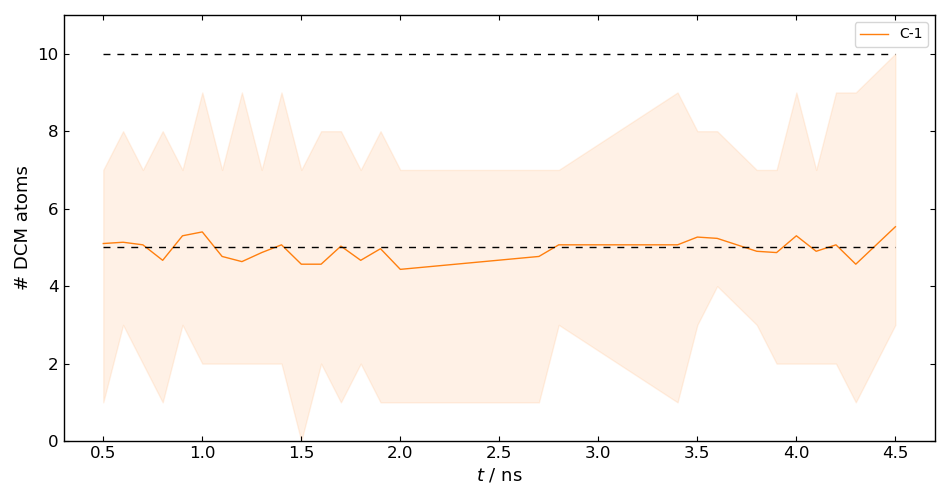
\includegraphics[width=13cm]{3/da//figs/figS14}
	\vspace{0.2cm}
	\hrule
	\caption{Temporal variation of the number of DCM solvent atoms ($n=5$ for one molecule of DCM) within the cavity of C-1 defined by the distance from the Pd--Pd midpoint to the nearest H atom (minus the vdW radius of H). Dashed lines correspond to one and two solvent molecules respectively.}
	\label{fig::si_da_14}
\end{figure}

From the proceeding discussion we have shown there to be differences with the treatment of the translational entropy and treatment of the low frequency modes, which dominate the free energy contribution. However, if the cage is considered to be occupied by a single solvent molecule, as confirmed by performing classical MD simulations in explicit DCM solvent, then the problematic treatment of the translational entropy is subject to a cancellation of errors, with no change in molecularity in the reaction: bq + DCM$\subset$C-X $\rightarrow$ bq$\subset$C-X + DCM.

% Don't remove me!
\clearpage 

\begin{figure}[h!]
	\vspace{0.4cm}
	\centering
	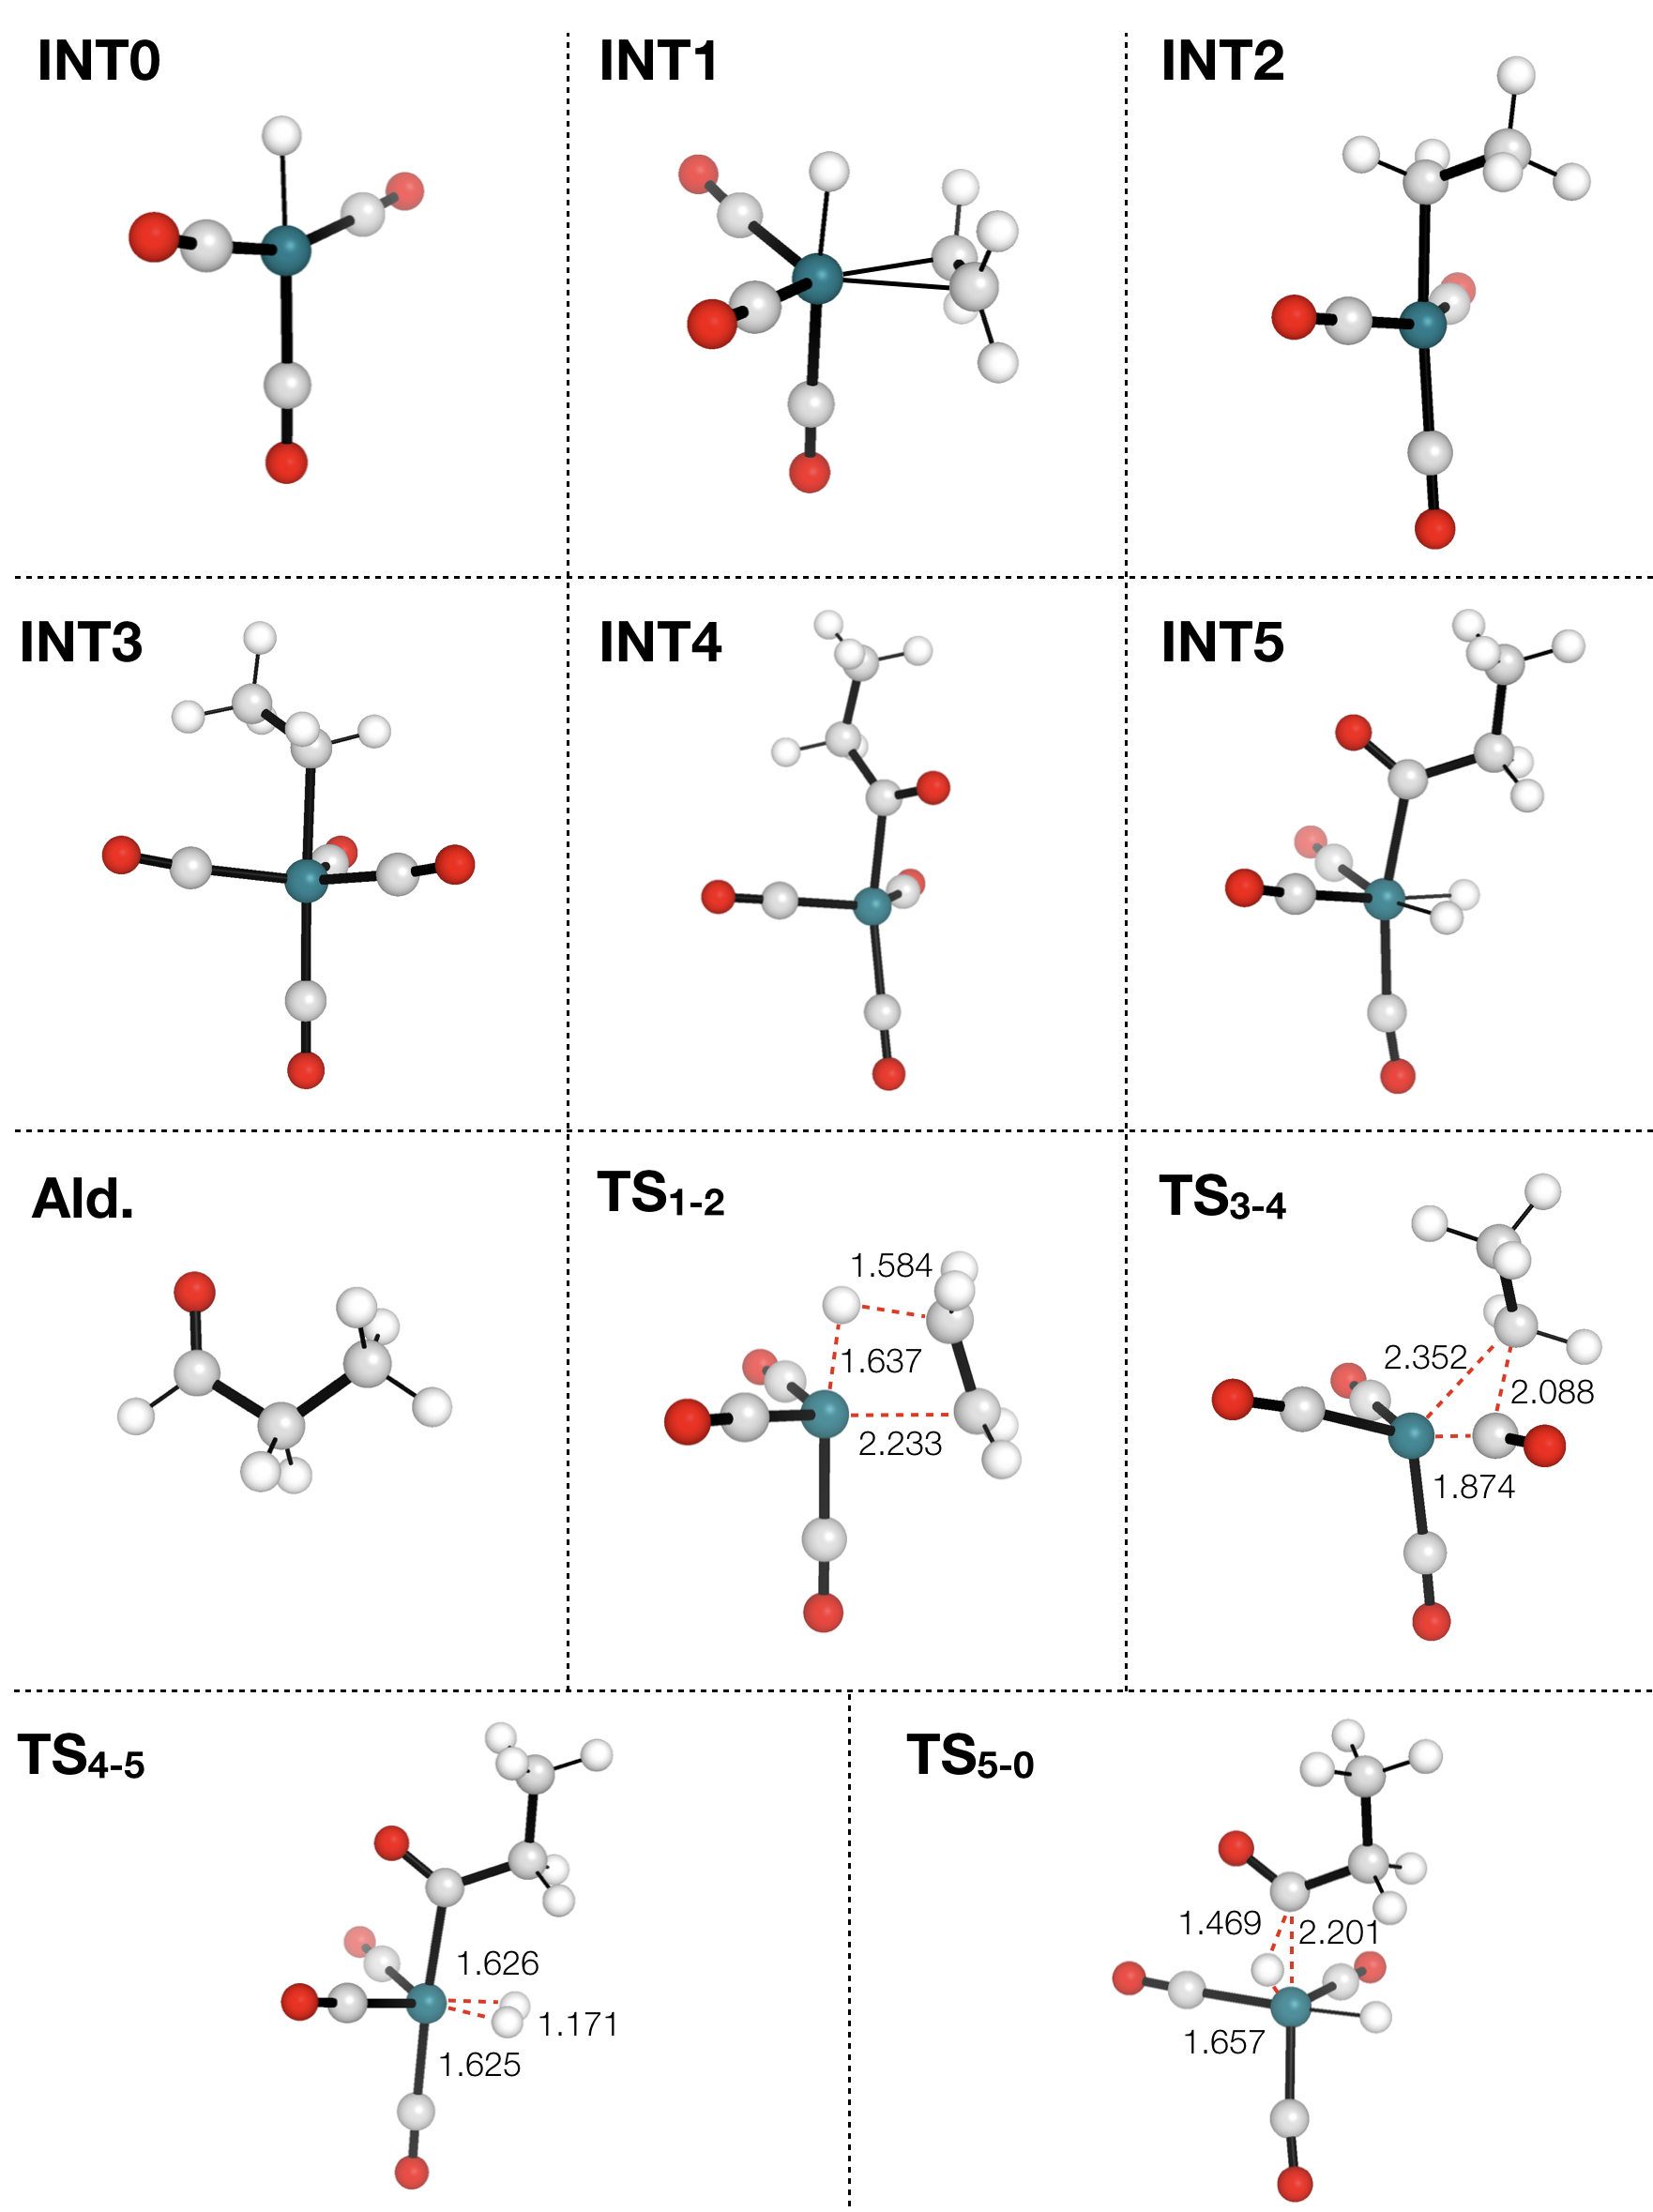
\includegraphics[width=13cm]{3/da//figs/figS15}
	\vspace{0.2cm}
	\hrule
	\caption{Quinones utilized in the binding affinity study.}
	\label{fig::si_da_15}
\end{figure}

\begin{table}[h!]
	\def\arraystretch{1.7}
	\begin{tabularx}{\textwidth}{YYYYYYYYY}
		\hline	
		&$H_\text{cont}$&	$TS_\text{trans}$	&$TS_\text{rot}	$&$TS_\text{vib}$&	$TS_\text{tot}$&$G_\text{cont}$  & $E_\text{bind}$ & $G_\text{bind}$  \\
		\hline
		
		{\small{DCM$\subset$
				C-1}}	&	734.9&	14.2&	12.9&	87.4&	114.4&	620.5	&&	
\\
		{\small{DCM$\subset$
				C-2}}		&	703.8&	14.2&	12.8&	85.2&	112.2&	591.6	&&	
\\
		{\small{DCM}}	                         & 21.3		&	11.7&	7.3	&0.7&	19.6&	1.7	&&	
\\
		{\small{$\Delta_\text{bind}$
				(bq$\subset$C-1)}}&	1.1	&-0.2	&-1.0&	0.7	&-0.5&	1.6  &	-3.0&	-1.4
\\
		{\small{$\Delta\Delta_\text{bind}$ 
				(bq$\subset$C-2)}}&	2.0	&-0.2&	-1.0&	1.5&	0.3&	1.6	&-4.8&	-3.2
\\
		{\small{$\Delta\Delta_\text{bind}$(bq)}}&		-0.9&	0.0	&0.0&	-0.9&	-0.9&	0.0&	-1.8&	-1.8
	
		
	\end{tabularx}
	\hrule
	\vspace{0.2cm}
	\caption{Thermodynamic contributions (\kcal) to the potential energy calculated at the PBE0-D3BJ/def2-SVP level of theory. $\Delta_\text{bind}$ = (bq$\subset$C-X + DCM) - (bq + DCM$\subset$C-X). Energies calculated at the SMD(DCM) M2/M1 level of theory. Note that the geometry optimized structures of DCM$\subset$C-1 and DCM$\subset$C-2 contained two and three imaginary modes respectively (all $<20$i cm$^{-1}$).}
	\label{table::si_da_7}
\end{table}


\begin{table}[h!]
	\def\arraystretch{1.7}
	\begin{tabularx}{\textwidth}{YYYYY}
		\hline	
		Cage&	Quinone	&calcd. $\Delta E_\text{bind}$	&expt.  $\Delta G_\text{bind}$&	AE \\
		\hline
		
		&q1	&-4.0&	-5.3&	1.3
\\
		&q2&	-7.5&	-7.4&	0.1
\\
		&q3&	-9.5&	-10.5&	1.0
\\
		&q4	&-14.6&	-12.2&	2.4
\\
	C-1 	&	q5&	-5.3&	-&	-
\\
 		&q6	&-6.8&	-&	-
\\
	&	q7	&-8.4&	-&	-
\\
	&	q8	&8.1&	-	&-
\\
	&	q9	&-8.6&	-3.6&	5.0
\\
		&q10&	-5.0&	-3.6	&1.4
\\
		
		&	q1&	-3.3&	-4.1&	0.8
\\
		&q2&	-6.1&	-4.7&	1.4
\\
		&	q3&	-6.8&	-5.4&	1.4
\\
		&	q4	&-11.2&-8.3	&2.9
\\
	C-2	&	q5&	-5.3&	-5.0&	0.3
\\
		&	q6	&-6.6&	-6.3&	0.3
\\
		&	q7	&-6.4&	-5.7&	0.7
\\
		&q8	&5.1	&    $\sim$0.0	&5.1
\\
		&	q9&	-7.1&	-&	-
\\
		&q10&	-3.4	&-	&-
\\
		MAE		&&&	&	1.7
\\

	\end{tabularx}
	\hrule
	\vspace{0.2cm}
	\caption{Calculated and experimental binding affinities for quinone substrates in cages C-1 and C-2 along with absolute errors (AE), and the mean absolute error. Experimental data from ref. \cite{August2016} for C-1, and ref 20 for C-2. this work. Absolute errors (AE) are calculated to experiment. All values in \kcal. $\Delta E_\text{bind}$ = $E_\text{M2/SMD(DCM)}$(qn$\subset$C-X) – [$E_\text{M2/SMD(DCM)}$(C-X) + $E_\text{M2/SMD(DCM)}$(qn)]. bq $\equiv$ q1 and aq $\equiv$ q3.}
	\label{table::si_da_8}
\end{table}


\begin{figure}[h!]
	\vspace{0.4cm}
	\centering
	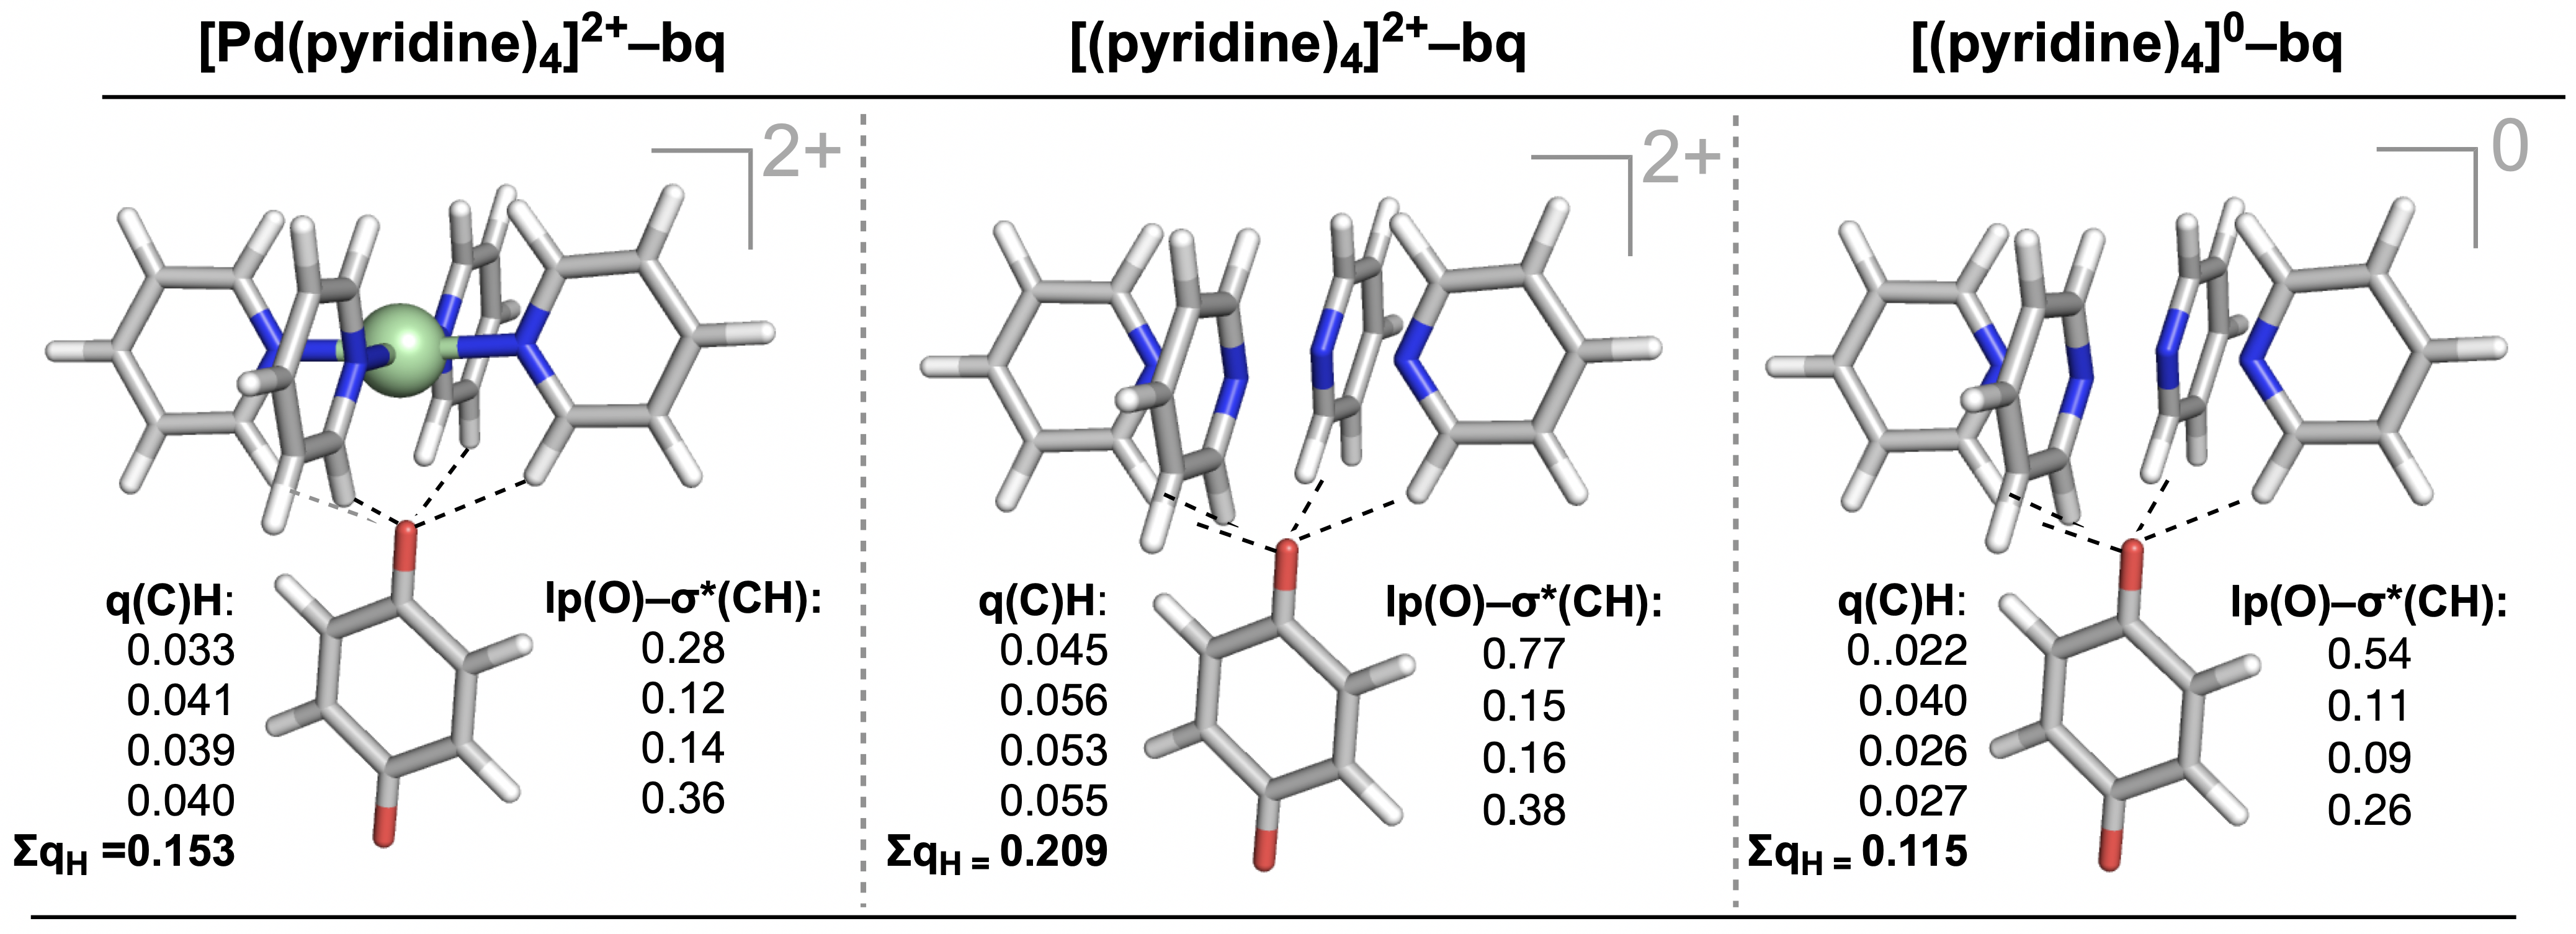
\includegraphics[width=\textwidth]{3/da//figs/figS16}
	\vspace{0.2cm}
	\hrule
	\caption{Comparison of atomic partial charges calculated using the Hirshfeld scheme and NBO second order perturbation decomposition calculated at the M06-2X/def2-TZVP level of theory. Charges are quoted in $e$ and interaction energies in \kcal.}
	\label{fig::si_da_16}
\end{figure}


\begin{figure}[h!]
	\vspace{0.4cm}
	\centering
	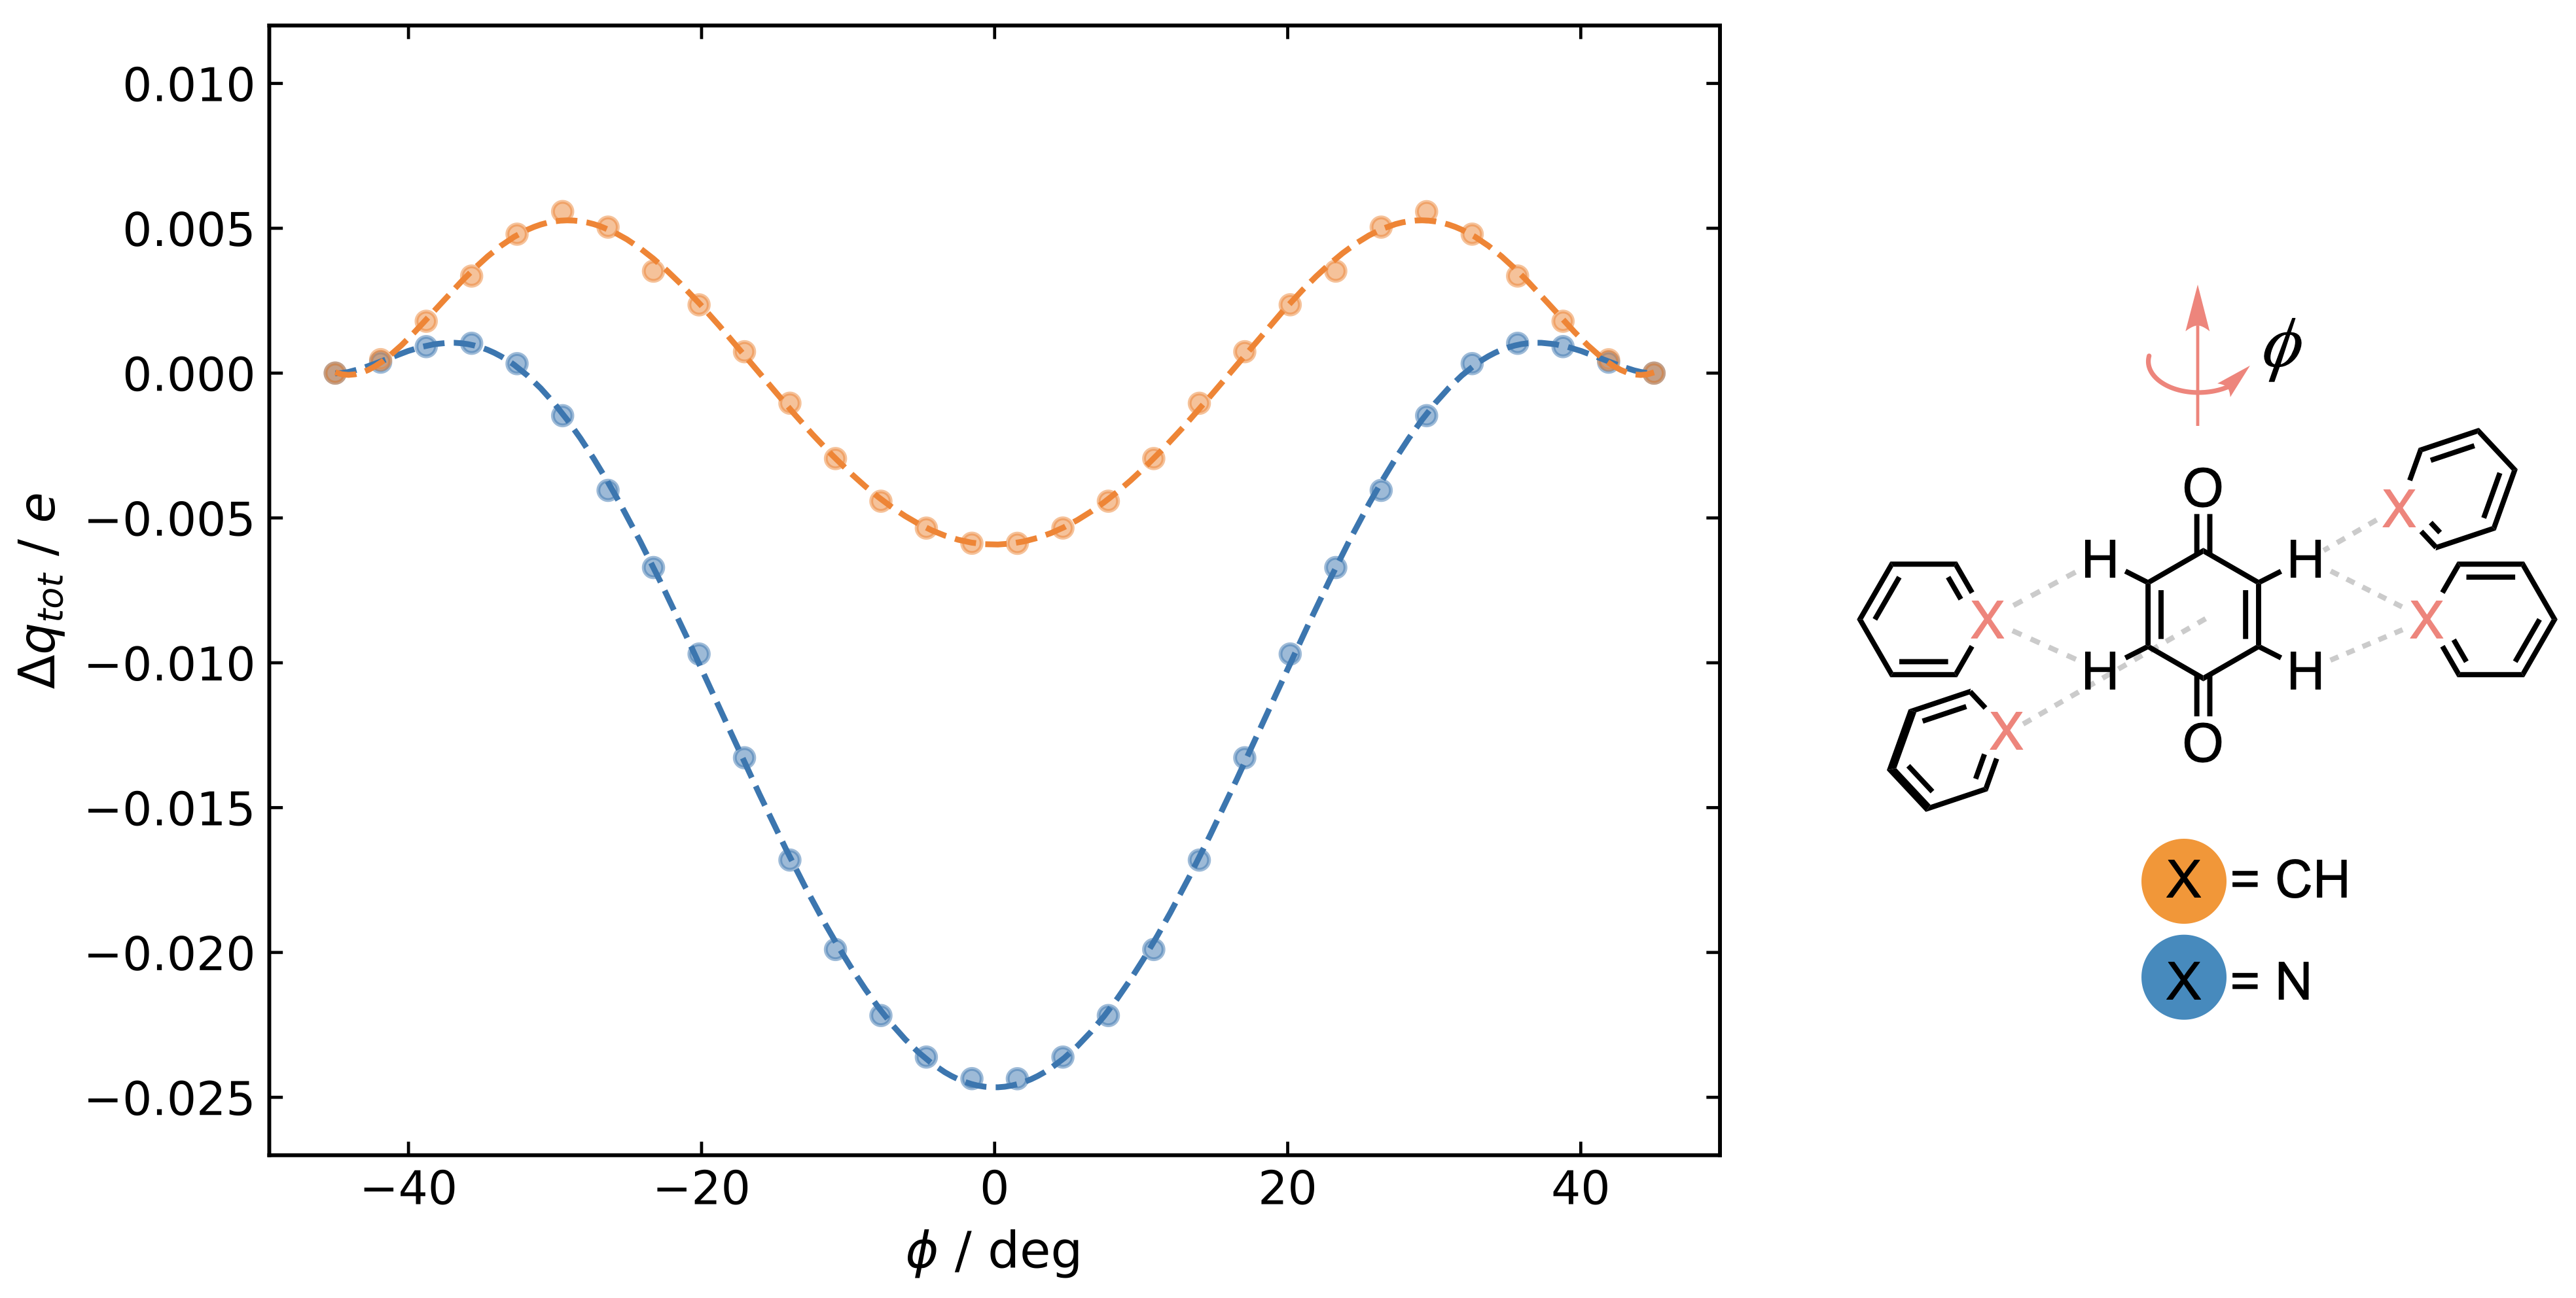
\includegraphics[width=15cm]{3/da//figs/figS17}
	\vspace{0.2cm}
	\hrule
	\caption{Total partial atomic charge on bq relative to $\phi = -45^\circ$ ($\Delta q_\text{tot}$) calculated with the Hirschfeld scheme at the M06-2X/def2-TZVP level of theory as a function of rotation around the z axis ($\phi$). $q_\text{tot} = \sum_i q_i$, where $i$ enumerates quinone atoms.}
	\label{fig::si_da_17}
\end{figure}


\begin{figure}[h!]
	\vspace{0.4cm}
	\centering
	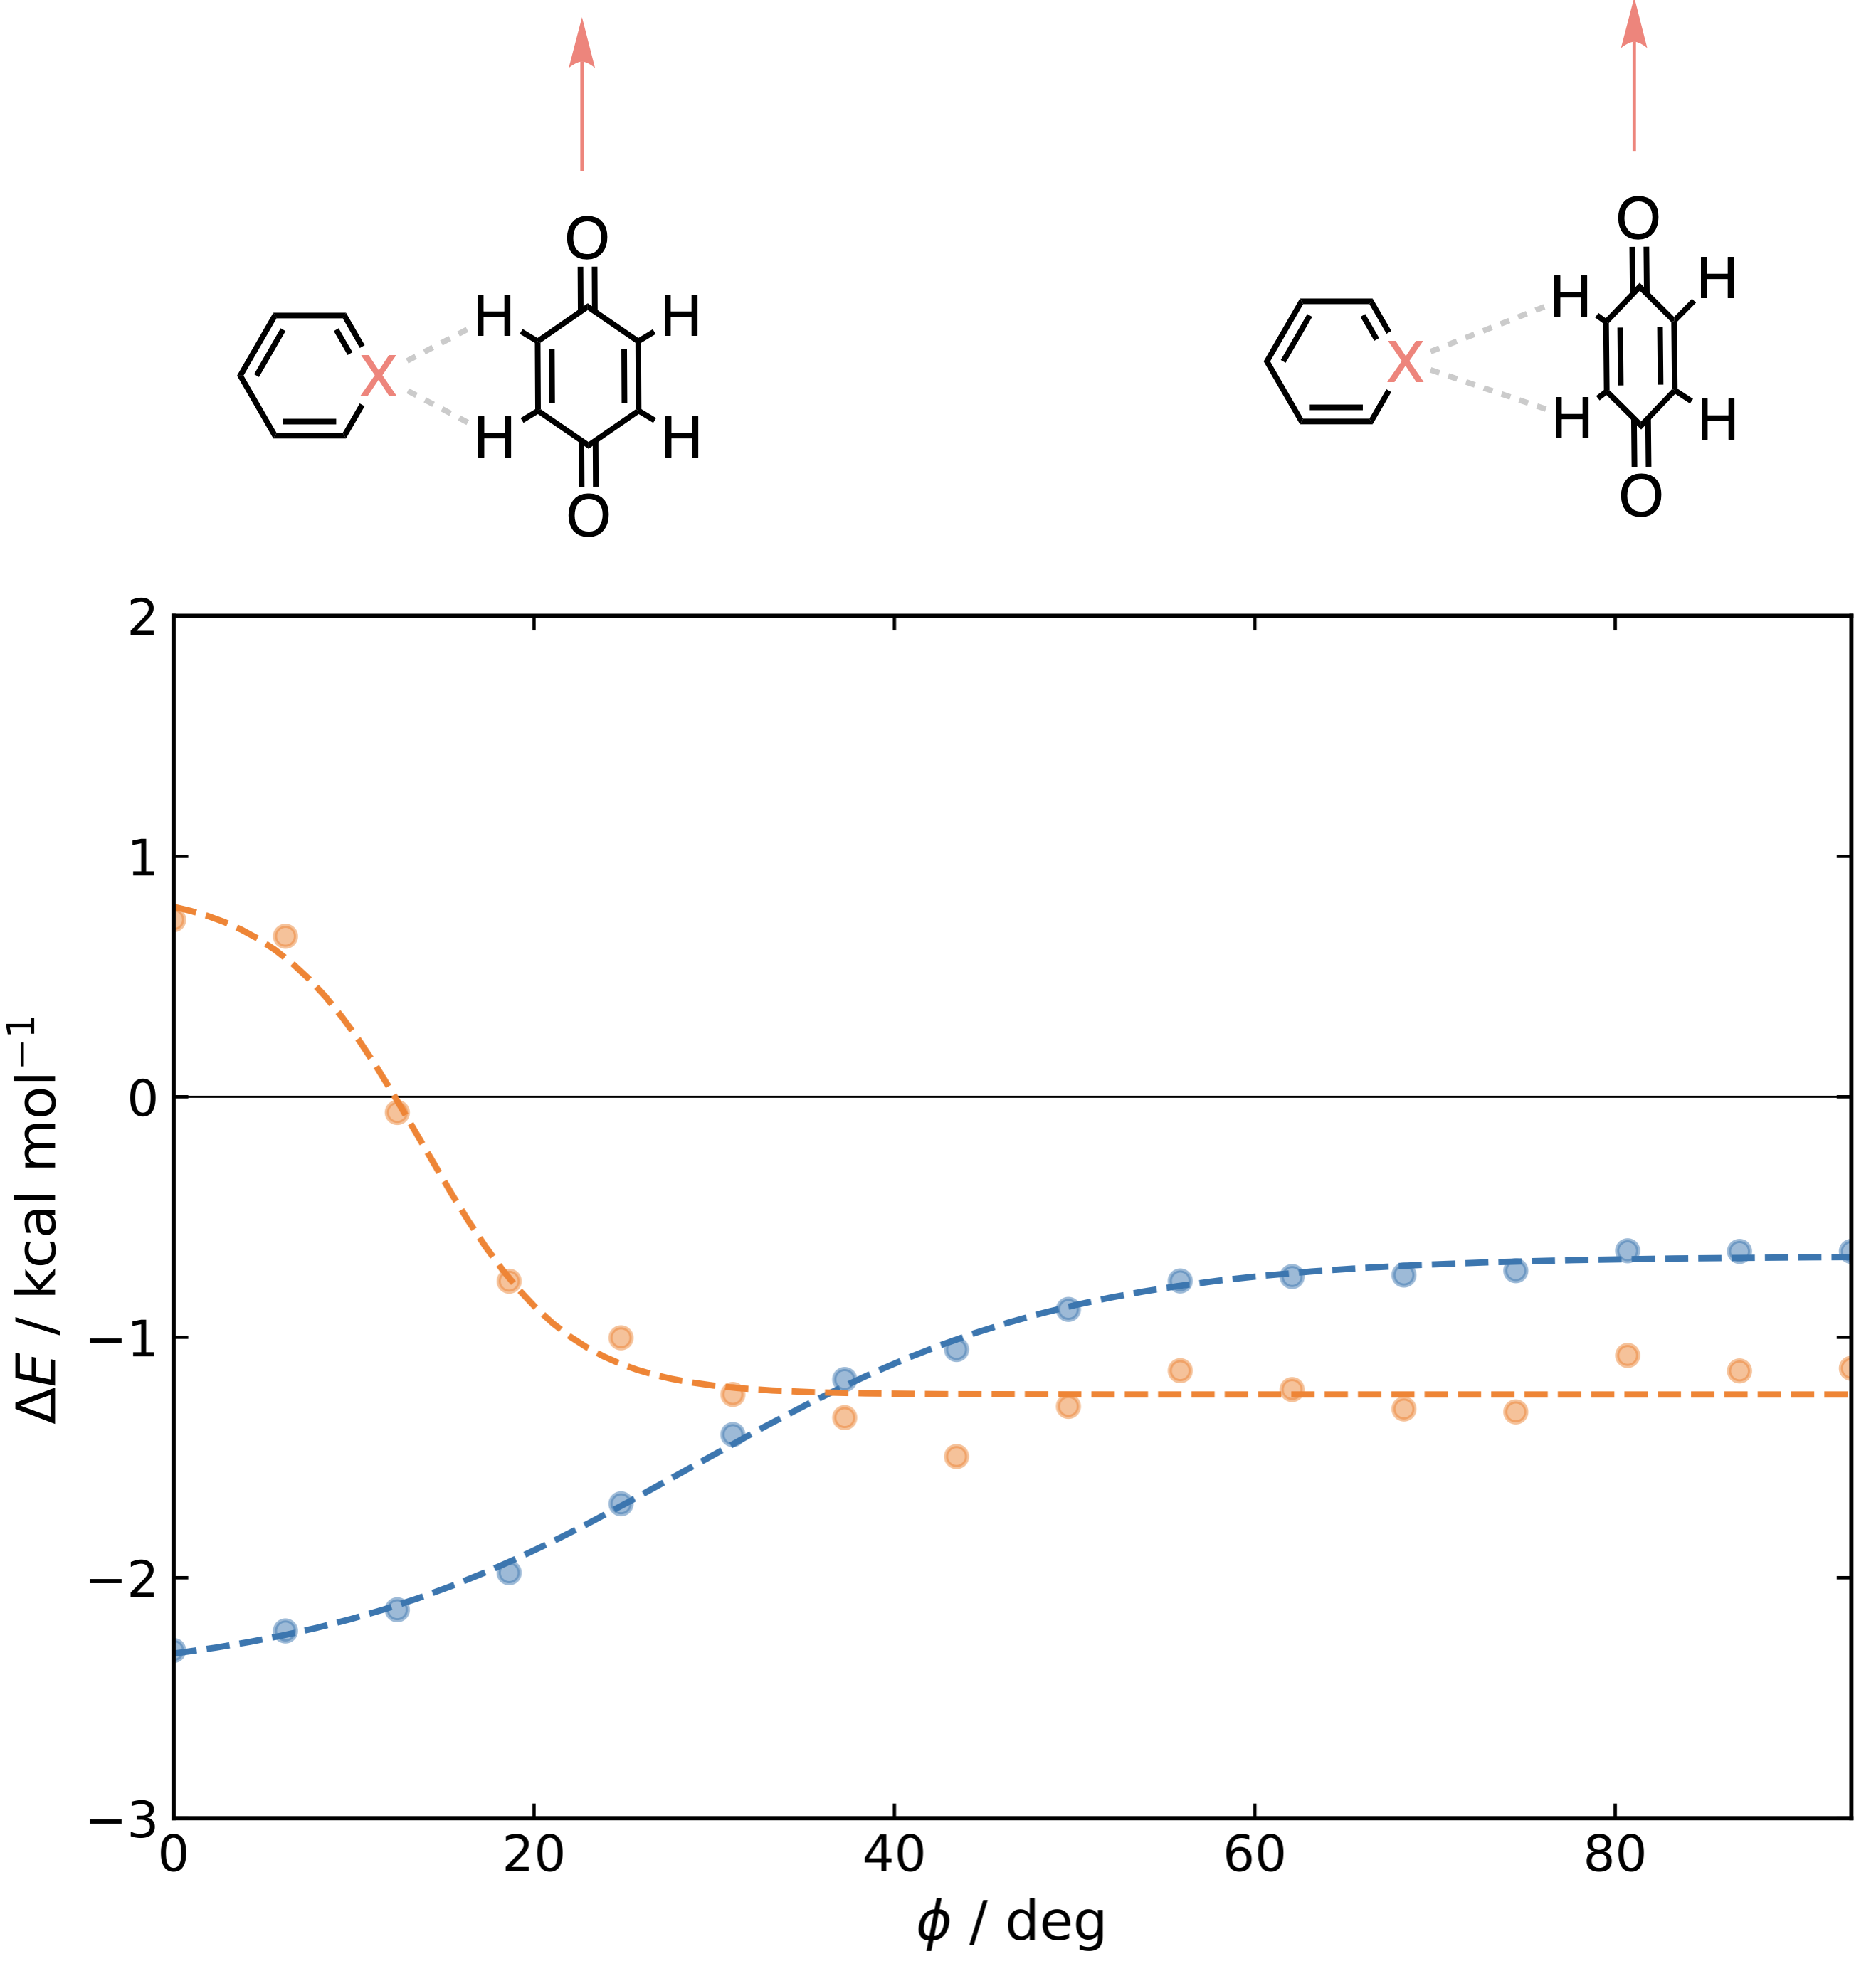
\includegraphics[width=11cm]{3/da//figs/figS18}
	\vspace{0.2cm}
	\hrule
	\caption{Relative energy (\kcal), calculated at the M06-2X/def2-TZVP level of theory, as a function of $\phi$ for a bq$\subset$benzene (orange) and bq$\subset$pyridine (blue) system.}
	\label{fig::si_da_18}
\end{figure}



\begin{figure}[h!]
	\vspace{0.4cm}
	\centering
	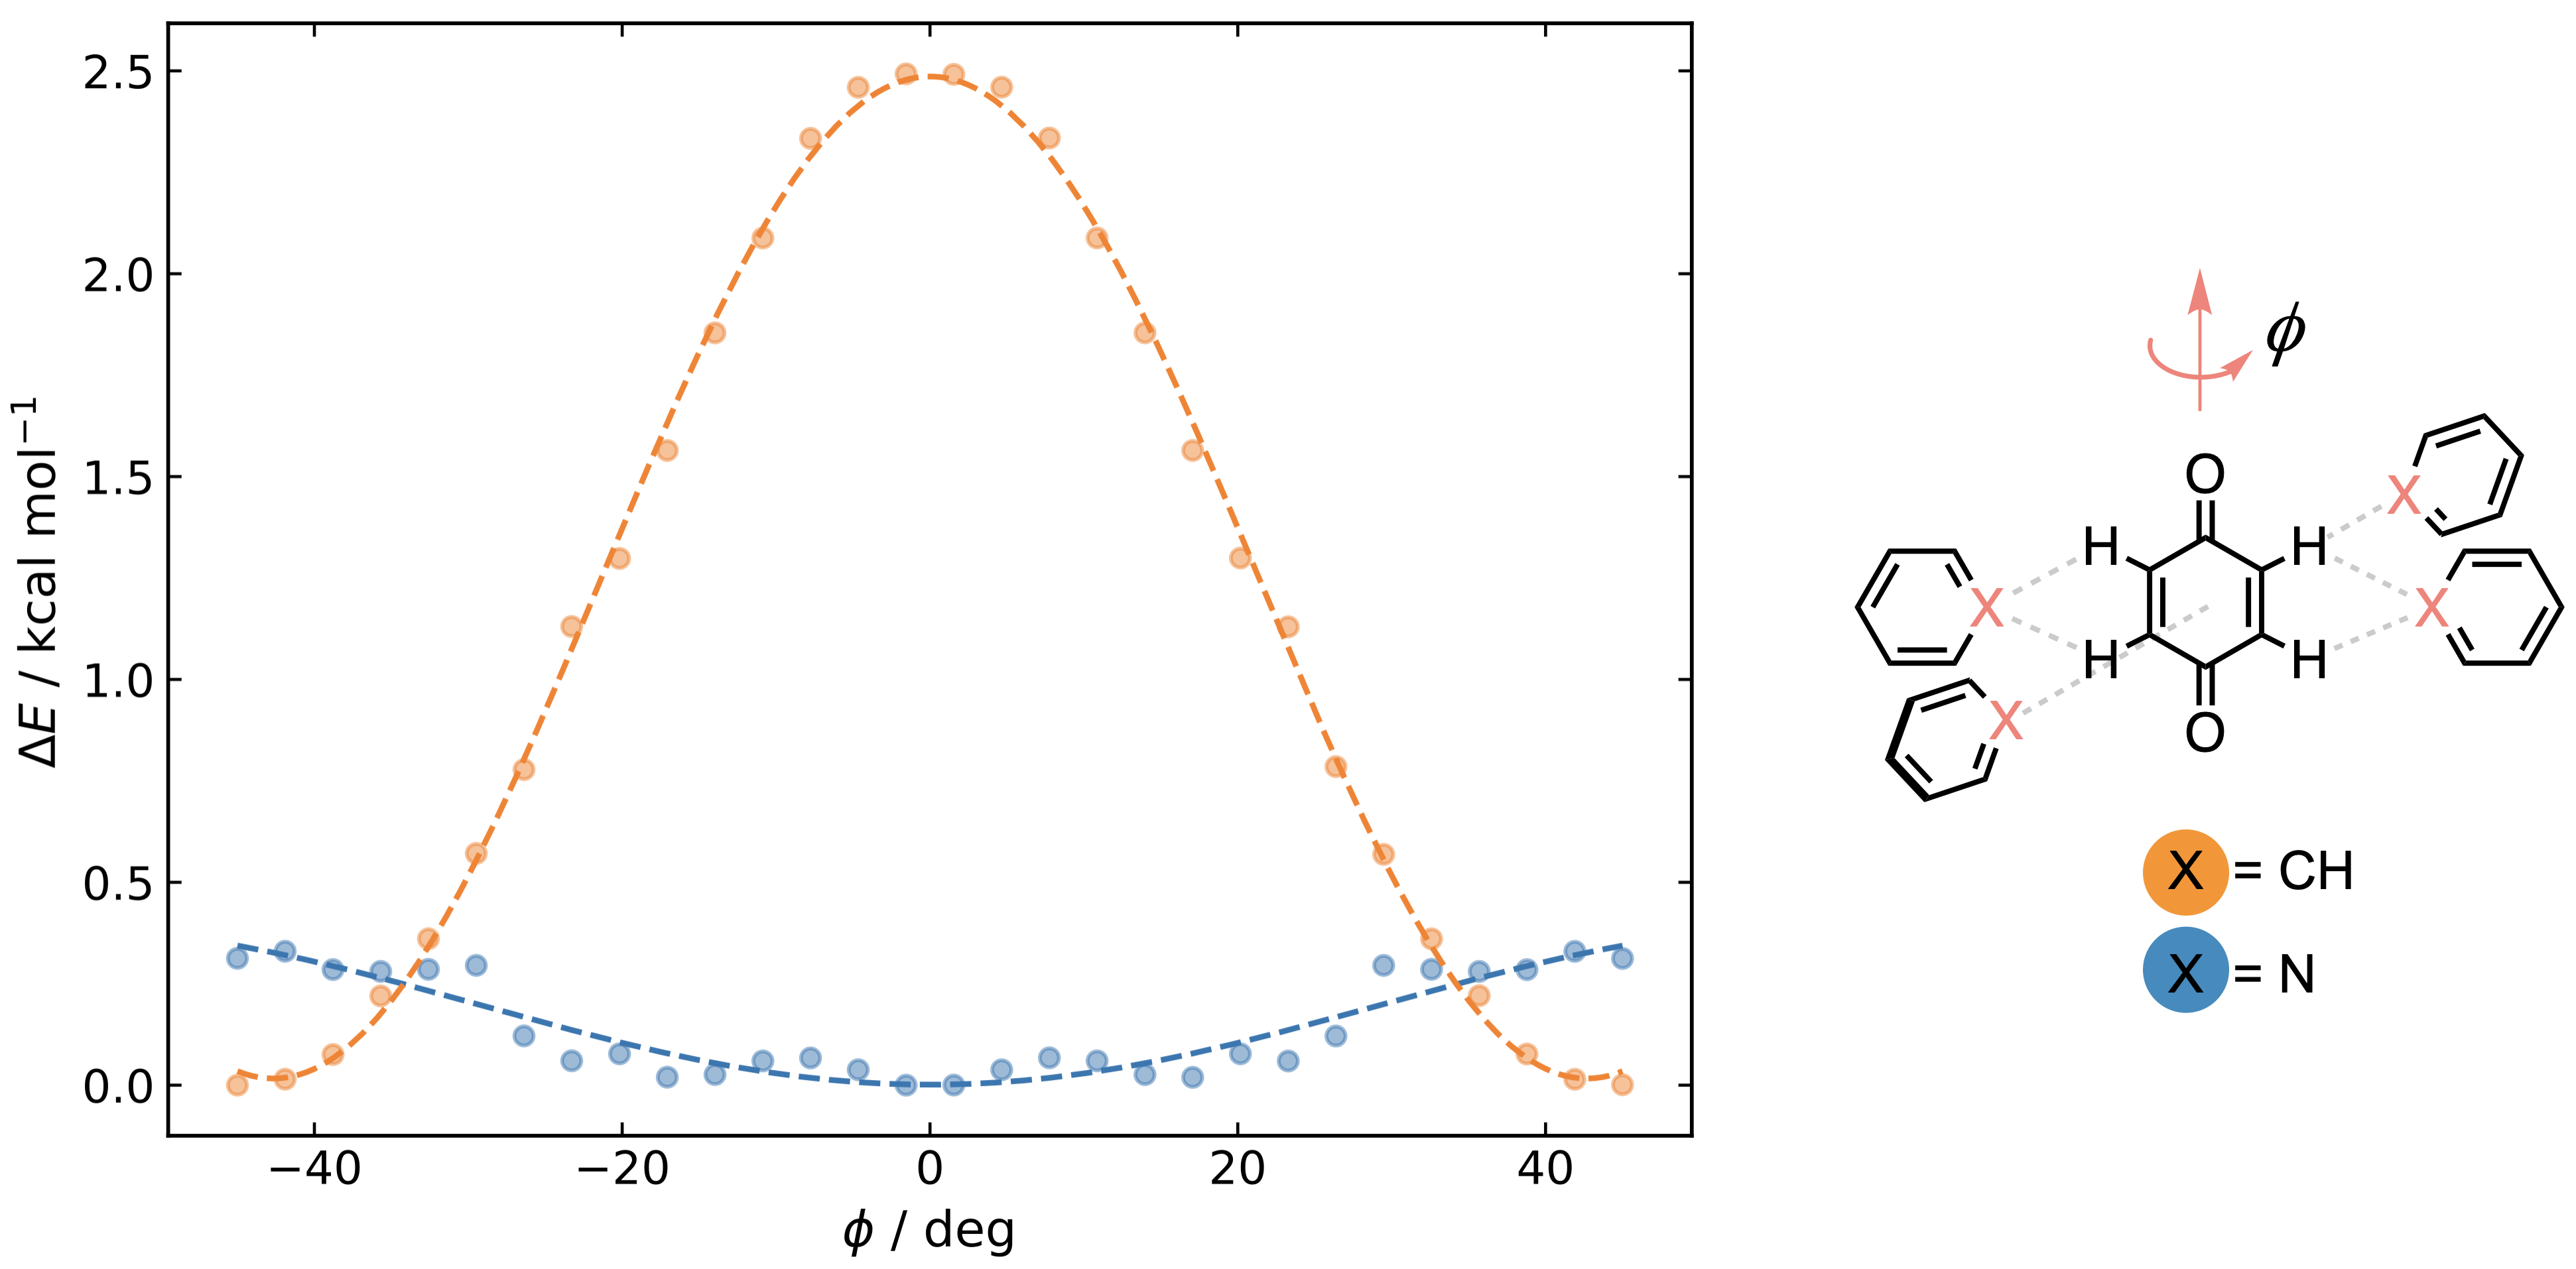
\includegraphics[width=\textwidth]{3/da//figs/figS19}
	\vspace{0.2cm}
	\hrule
	\caption{Relative energy (\kcal), calculated at the SMD(DCM)-M06-2X/def2-TZVP level of theory, as a function of $\phi$ for a bq$\subset$benzene (orange) and bq$\subset$pyridine (blue) system. Implicit solvent considerably reduces the pyridine–bq interaction while the Pauli repulsion is not modulated by the solvent.}
	\label{fig::si_da_19}
\end{figure}



\begin{figure}[h!]
	\vspace{0.4cm}
	\centering
	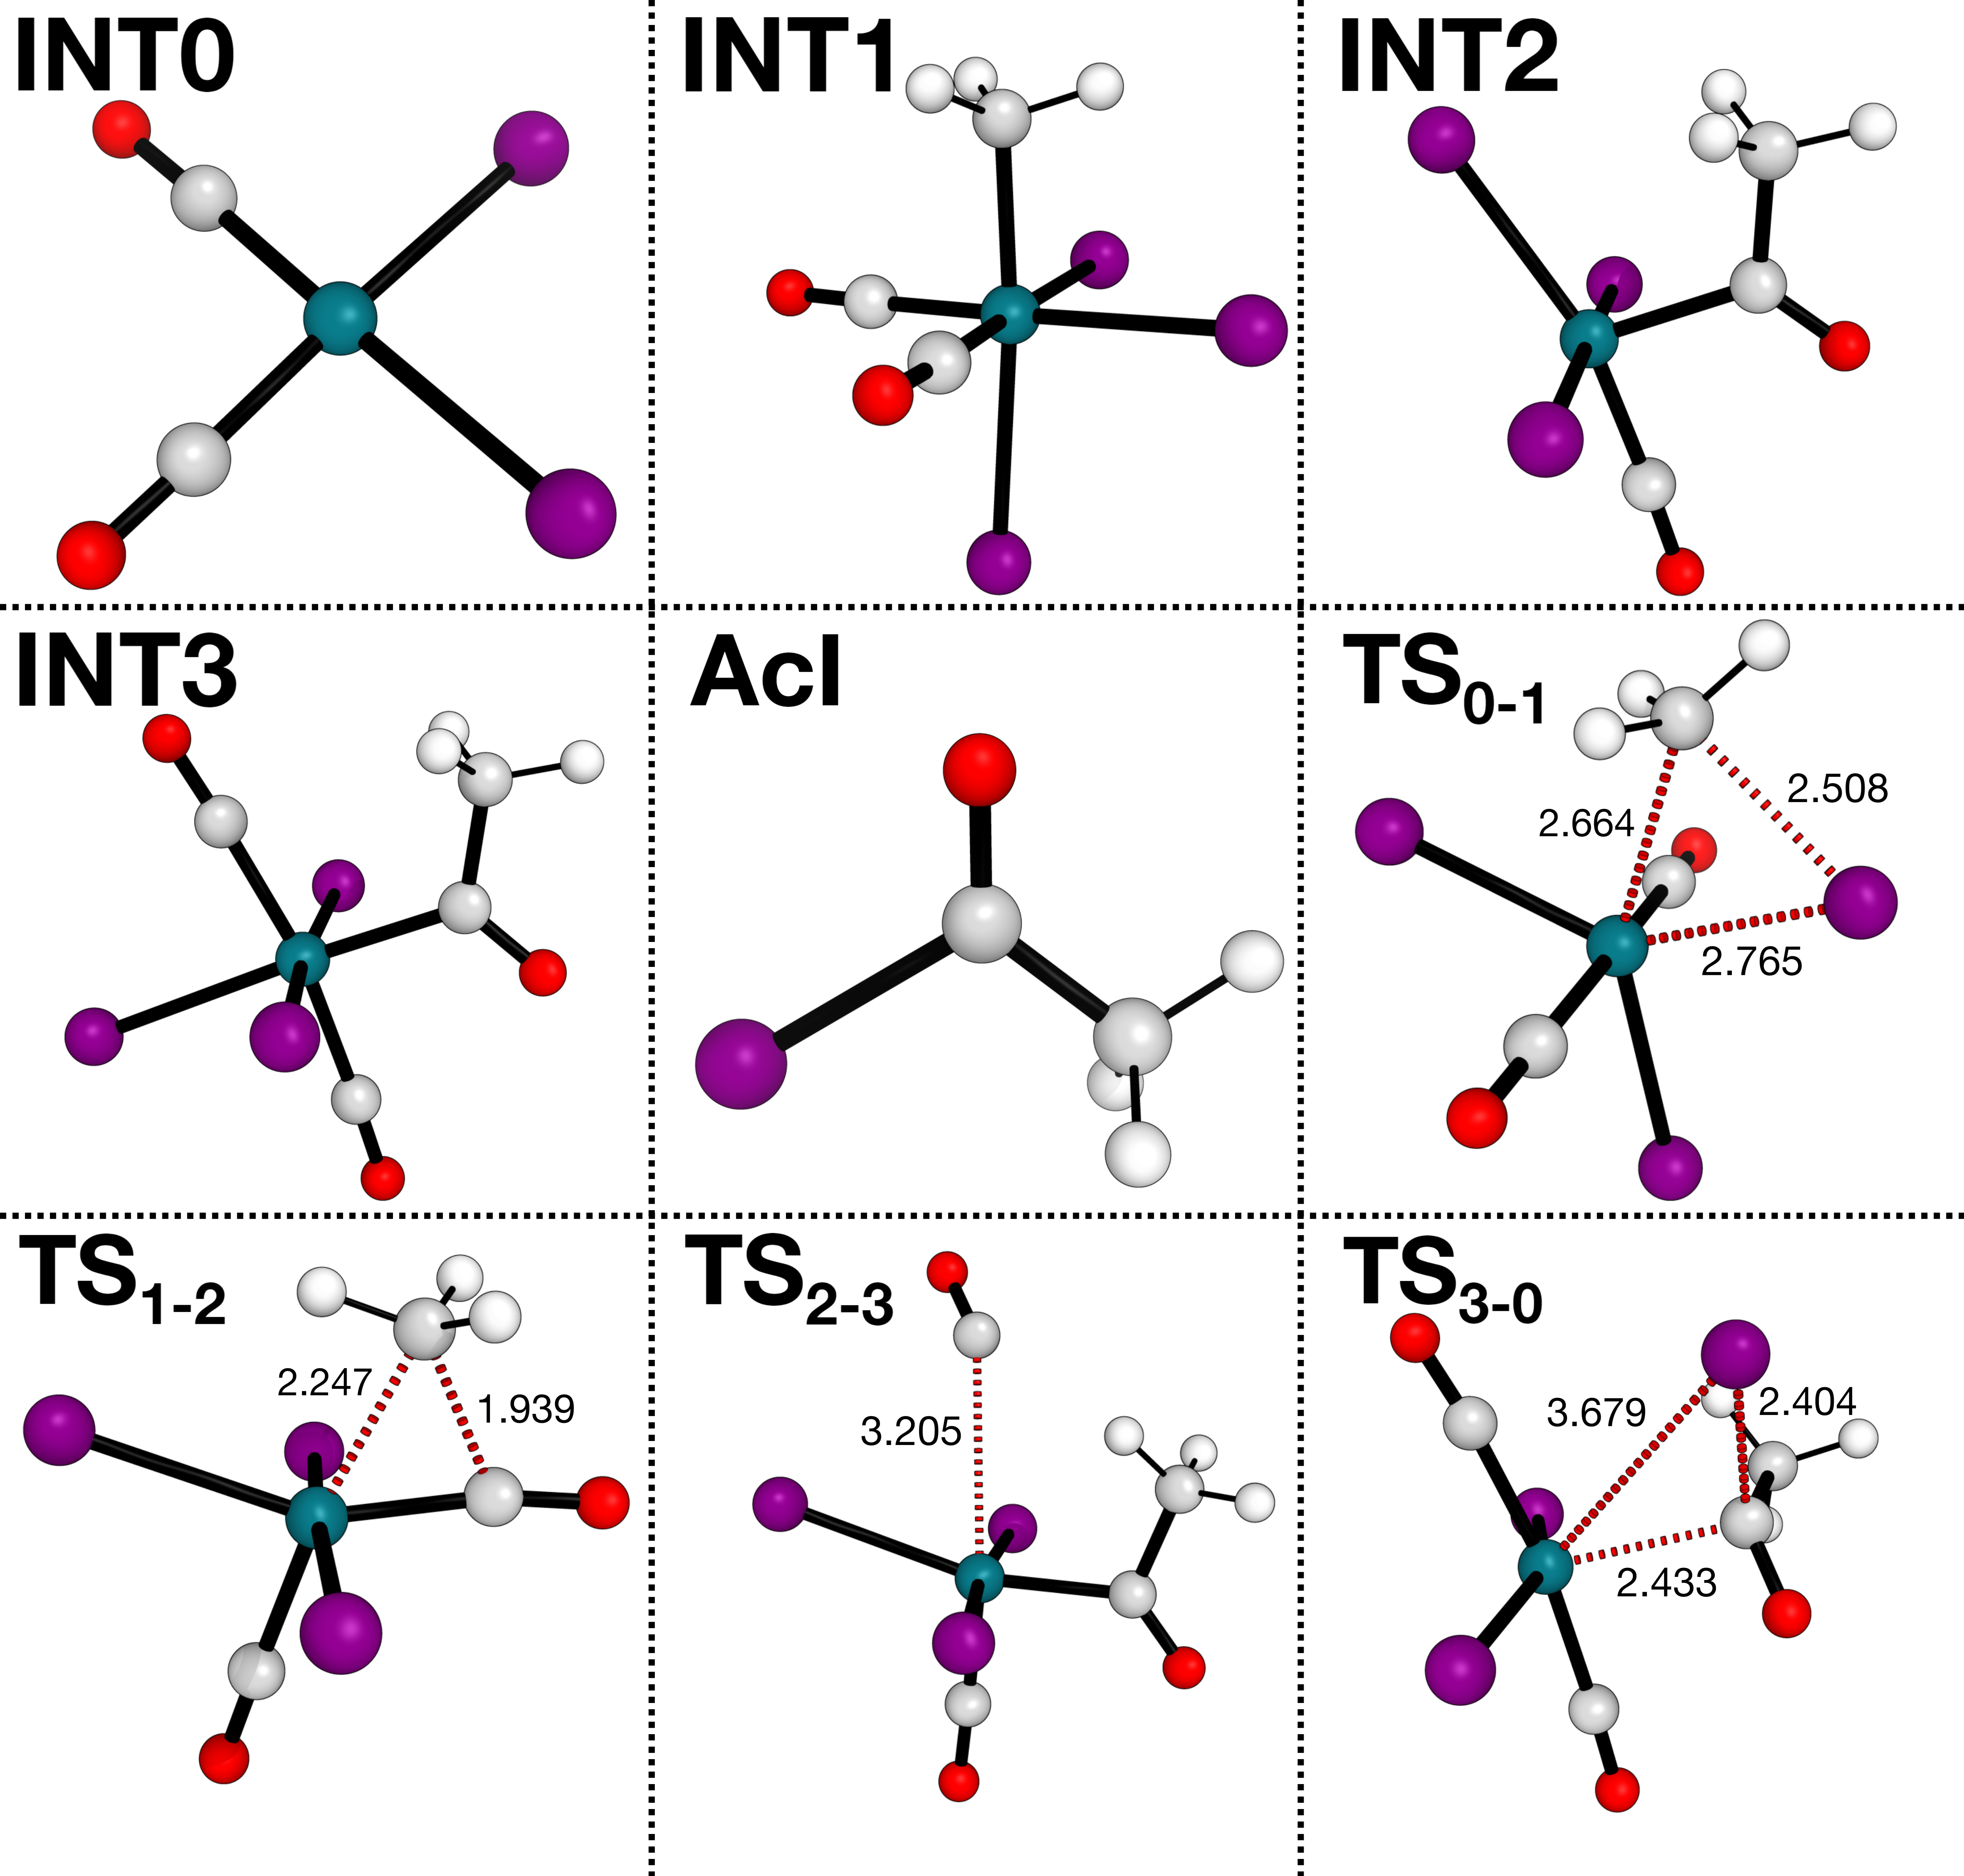
\includegraphics[width=13cm]{3/da//figs/figS20}
	\vspace{0.2cm}
	\hrule
	\caption{Quinones and dienes for a representative set of 10 uncatalysed Diels–Alder (DA) reactions reported in ref. \cite{MartCentelles2018}.}
	\label{fig::si_da_20}
\end{figure}



\begin{figure}[h!]
	\vspace{0.4cm}
	\centering
	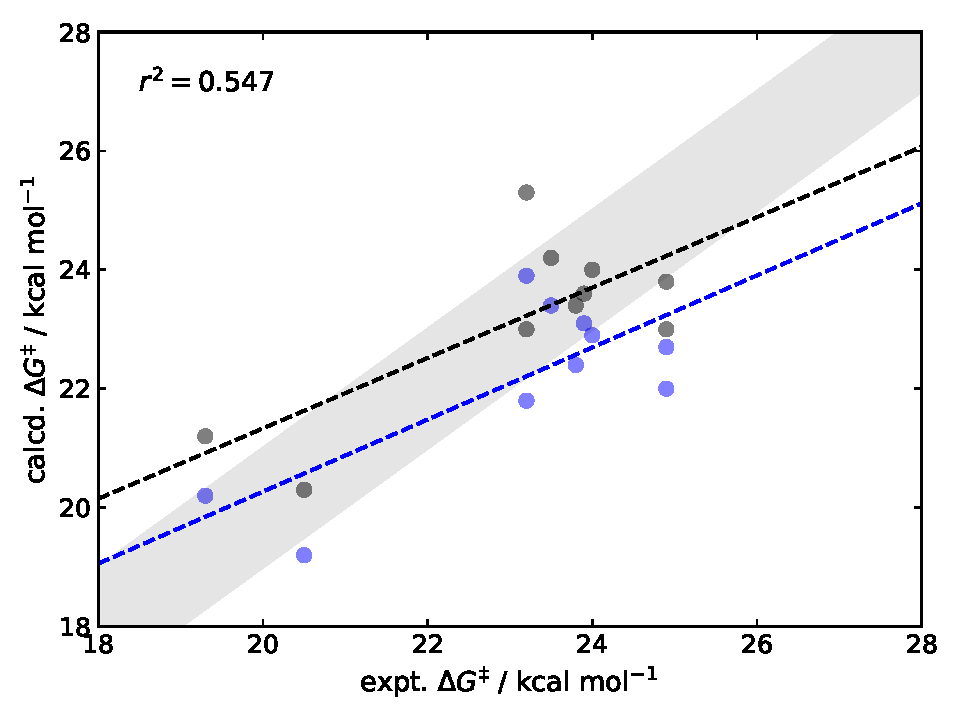
\includegraphics[width=10cm]{3/da//figs/figS21}
	\vspace{0.2cm}
	\hrule
	\caption{Correlation plot of the gas phase $\Delta G^\ddagger$ (black) and solvated $\Delta G^\ddagger_\text{solv.}$ (blue) activation energies for the uncatalysed endo-DA reactions (data reported in Table \ref{table::si_da_11_12}). Correlation coefficients are identical. Grey diagonal area indicates the $\pm$1 \kcalx area of accuracy.}
	\label{fig::si_da_21}
\end{figure}


\begin{figure}[h!]
	\vspace{0.4cm}
	\centering
	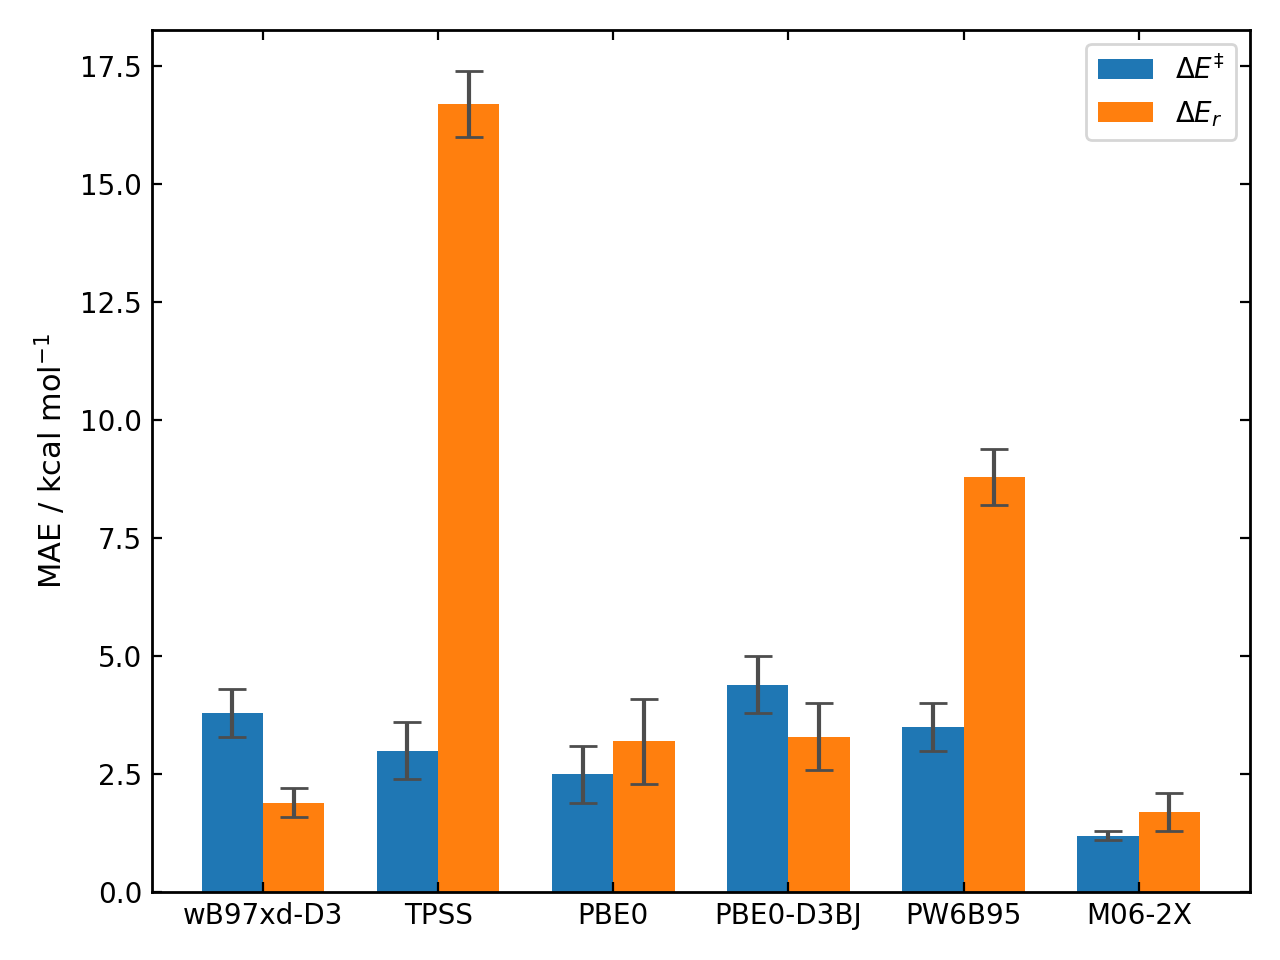
\includegraphics[width=11cm]{3/da//figs/figS22}
	\vspace{0.2cm}
	\hrule
	\caption{Mean absolute deviations to DLPNO-CCSD(T)/ma-def2-TZVPP potential energy differences for reaction barriers ($\Delta E^\ddagger$), and reaction energies ($\Delta E_r$) for a set of 10 Diels Alder reactions outlined in Table \ref{table::si_da_3}. Error bars are std. error in the mean.}
	\label{fig::si_da_22}
\end{figure}



\begin{table}[h!]
	\def\arraystretch{1.7}
	\begin{tabularx}{\textwidth}{YYYYYYY}
		\hline
		Diene	&Dienophile	&$\Delta E^\ddagger$ &$\Delta H^\ddagger$&	$\Delta G^\ddagger$	&$\Delta G^\ddagger_\text{solv}$&	$\Delta G^\ddagger_\text{expt}$ \\
		\hline
		d1	&q1	&11.0&11.9	&24.0&22.9&	24.0
\\
		d1&	q5	&10.7	&11.5&	23.8	&22.7&	24.9
\\
		d1	&q8&9.8	&10.6&	23.0&	22.0&	24.9
\\
		d2&	q1	&8.4&	9.4	&21.2&	20.2&	19.3
\\
		d2	&q2	&7.2	&8.2&	20.3&	19.2&	20.5
\\
		d2	&q6	&10.9&	11.9&	24.2&	23.4&	23.5
\\
		d2	&q7	&10.2&	11.2	&23.6&	23.1&	23.9
\\
		d3&	q1	&12.5	&13.5&	25.3&	23.9&	23.2
\\
		d4&	q5&	9.8	   &10.6&	23.4&	22.4&	23.8
\\
		d5&	q1	&9.0&	9.9	&23.0	&21.8& 	23.2
\\
		&&&&&&\\
		\hline
		&&$\Delta E_r$ &$\Delta H_r$&	$\Delta G_r$	&$\Delta G_\text{solv}$&\\
		\hline
		d1	&q1	&-45.0	&-41.1&	-28.1&	-27.3&
\\
		d1	&q5&	-45.1	&-41.2&	-28.1&	-27.3&
\\
		d1	&q8&	-45.1&	-41.2&	-27.9&	-27.1&\\
		d2&	q1	&-27.5&	-23.9&	-11.2&	-10.4&
\\
		d2	&q2	&-27.2&	-23.6&	-10.7&	-10.1
&\\
		d2	&q6	&-25.1&	-21.7&	-8.4&	-7.3&
\\
		d2	&q7	&-24.4&	-21.0&	-7.7&	-6.4
&\\
		d3&	q1	&-34.4&	-30.8	&-17.8	&-16.9
&\\
		d4&	q5	&-41.2&	-37.3&	-23.7&	-22.7&
\\
		d5	&q1	&-41.0&	-37.1&	-23.4&	-22.5&
\\
	\end{tabularx}
	\hrule
	\vspace{0.2cm}
	\caption{Gas phase and solvated($\Delta G^\ddagger_\text{solv}$) activation energies (\kcal) for the uncatalysed endo-DA reactions calculated at the DLPNO-CCSD(T)/ma-def2-TZVPP//PBE0-D3BJ/def2-SVP level of theory with thermodynamic and solvation contributions calculated at PBE0 D3BJ/def2-SVP with the 1M standard state correction, and SMD(DCM)-PBE0 D3BJ/def2 SVP/ respectively.}
	\label{table::si_da_11_12}
\end{table}



\begin{table}[h!]
	\def\arraystretch{1.7}
	\begin{tabularx}{\textwidth}{YYYYYY}
		\hline
		Diene	&Dienophile	&$\Delta E^\ddagger$ &$\Delta H^\ddagger$&	$\Delta G^\ddagger$	&$\Delta G^\ddagger_\text{solv}$ \\
		\hline
		d1&	q1	&29.2&	26.3&	-25.2&	-28.1
\\
		d1	&q5	&29.4&	26.2&	-25.1&	-28.1
\\
		d1&	q8	&29.0&	25.1&	-25.1&	-28.9\\
		d2&	q1	&27.2&	24.2&	-7.0&	-9.4
\\
		d2&	q2	&26.5&	21.5&	-6.2&	-10.6
\\
		d2&	q6	&30.1	&27.0&	-4.3&	-6.9
\\
		d2&	q7	&29.1&	24.3&	-3.4&	-7.4
\\
		d3&	q1	&32.4&	29.2&	-13.8&	-16.7
\\
		d4&	q5	&28.8&	26.1&	-23.1&	-25.8
\\
		d5&	q1	&28.2	&23.7&	-23.9&	-28.2\\
	\end{tabularx}
	\hrule
	\vspace{0.2cm}
	\caption{Gas phase and solvated($\Delta G^\ddagger_\text{solv}$) activation energies (\kcal) for the uncatalysed exo-DA reactions calculated at the DLPNO-CCSD(T)/ma-def2-TZVPP//PBE0-D3BJ/def2-SVP level of theory with thermodynamic and solvation contributions calculated at PBE0 D3BJ/def2-SVP with the 1M standard state correction, and SMD(DCM)-PBE0 D3BJ/def2 SVP/ respectively.}
	\label{table::si_da_15}
\end{table}


\clearpage   % Don't delete me, required for formatting


First, the most stable species or set of species available to the C-2, bq, isoprene in DCM system is found, from which the TS likely occurs. We assume that a pre-equilibrium is established quickly, with all energetic barriers being smaller than the for the DA reaction between isoprene and bq. Due to the conformational flexibility of L${}^\text{CH}$/L${}^\text{N}$, other arrangements of the reactants inside the cage, including binding of both the diene and dienophile is also possible. However, they were found to have higher energies both at the complex and TS stage. 

The increased electrophilicity of the quinone within the cage can be quantified by the total effective charge of bq within C-1/C-2 (relative to its neutral form in solution). Within C-1/C-2 bq has a slightly positive charge – indicating that the +4 cage removes some electron density from bq, thereby activating it as a dienophile. This effect is slightly more pronounced in C-1 across the different decomposition schemes.



\begin{table}[h!]
	\def\arraystretch{1.7}
	\begin{tabularx}{\textwidth}{YYYY}
		\hline
		Species&	$\Delta E$	&$\Delta H$	&$\Delta G$
\\
		\hline
		bq$\subset$C-2	&0.0&	0.0&	0.0
\\
		d1$\subset$C-2a &3.7&	2.3	&1.3
\\
		bq.d1$\subset$C-2	&-6.4&	-4.4&	8.8
\\
		
	\end{tabularx}
	\hrule
	\vspace{0.2cm}
	\caption{Energies of possible complexes relative to bq$\subset$C-2.}
	\label{table::si_da_16}
\end{table}


To assess the effect the C-H$\cdots$O interactions play in enhancing the electrophilic character an electron density difference map (EDDM)  is generated between the electron density of bq$\subset$C-2 and the electron density of bq (neutral) and C-2 (4+ charge) at the PBE0-D3BJ/def2-SVP level of theory. The resultant EDDM is shown in Figure \ref{fig::si_da_24} and shows how the C(2)–Hs present in the donor pyridines remove electron density away from the carbonyls.

\begin{figure}[h!]
	\vspace{0.4cm}
	\centering
	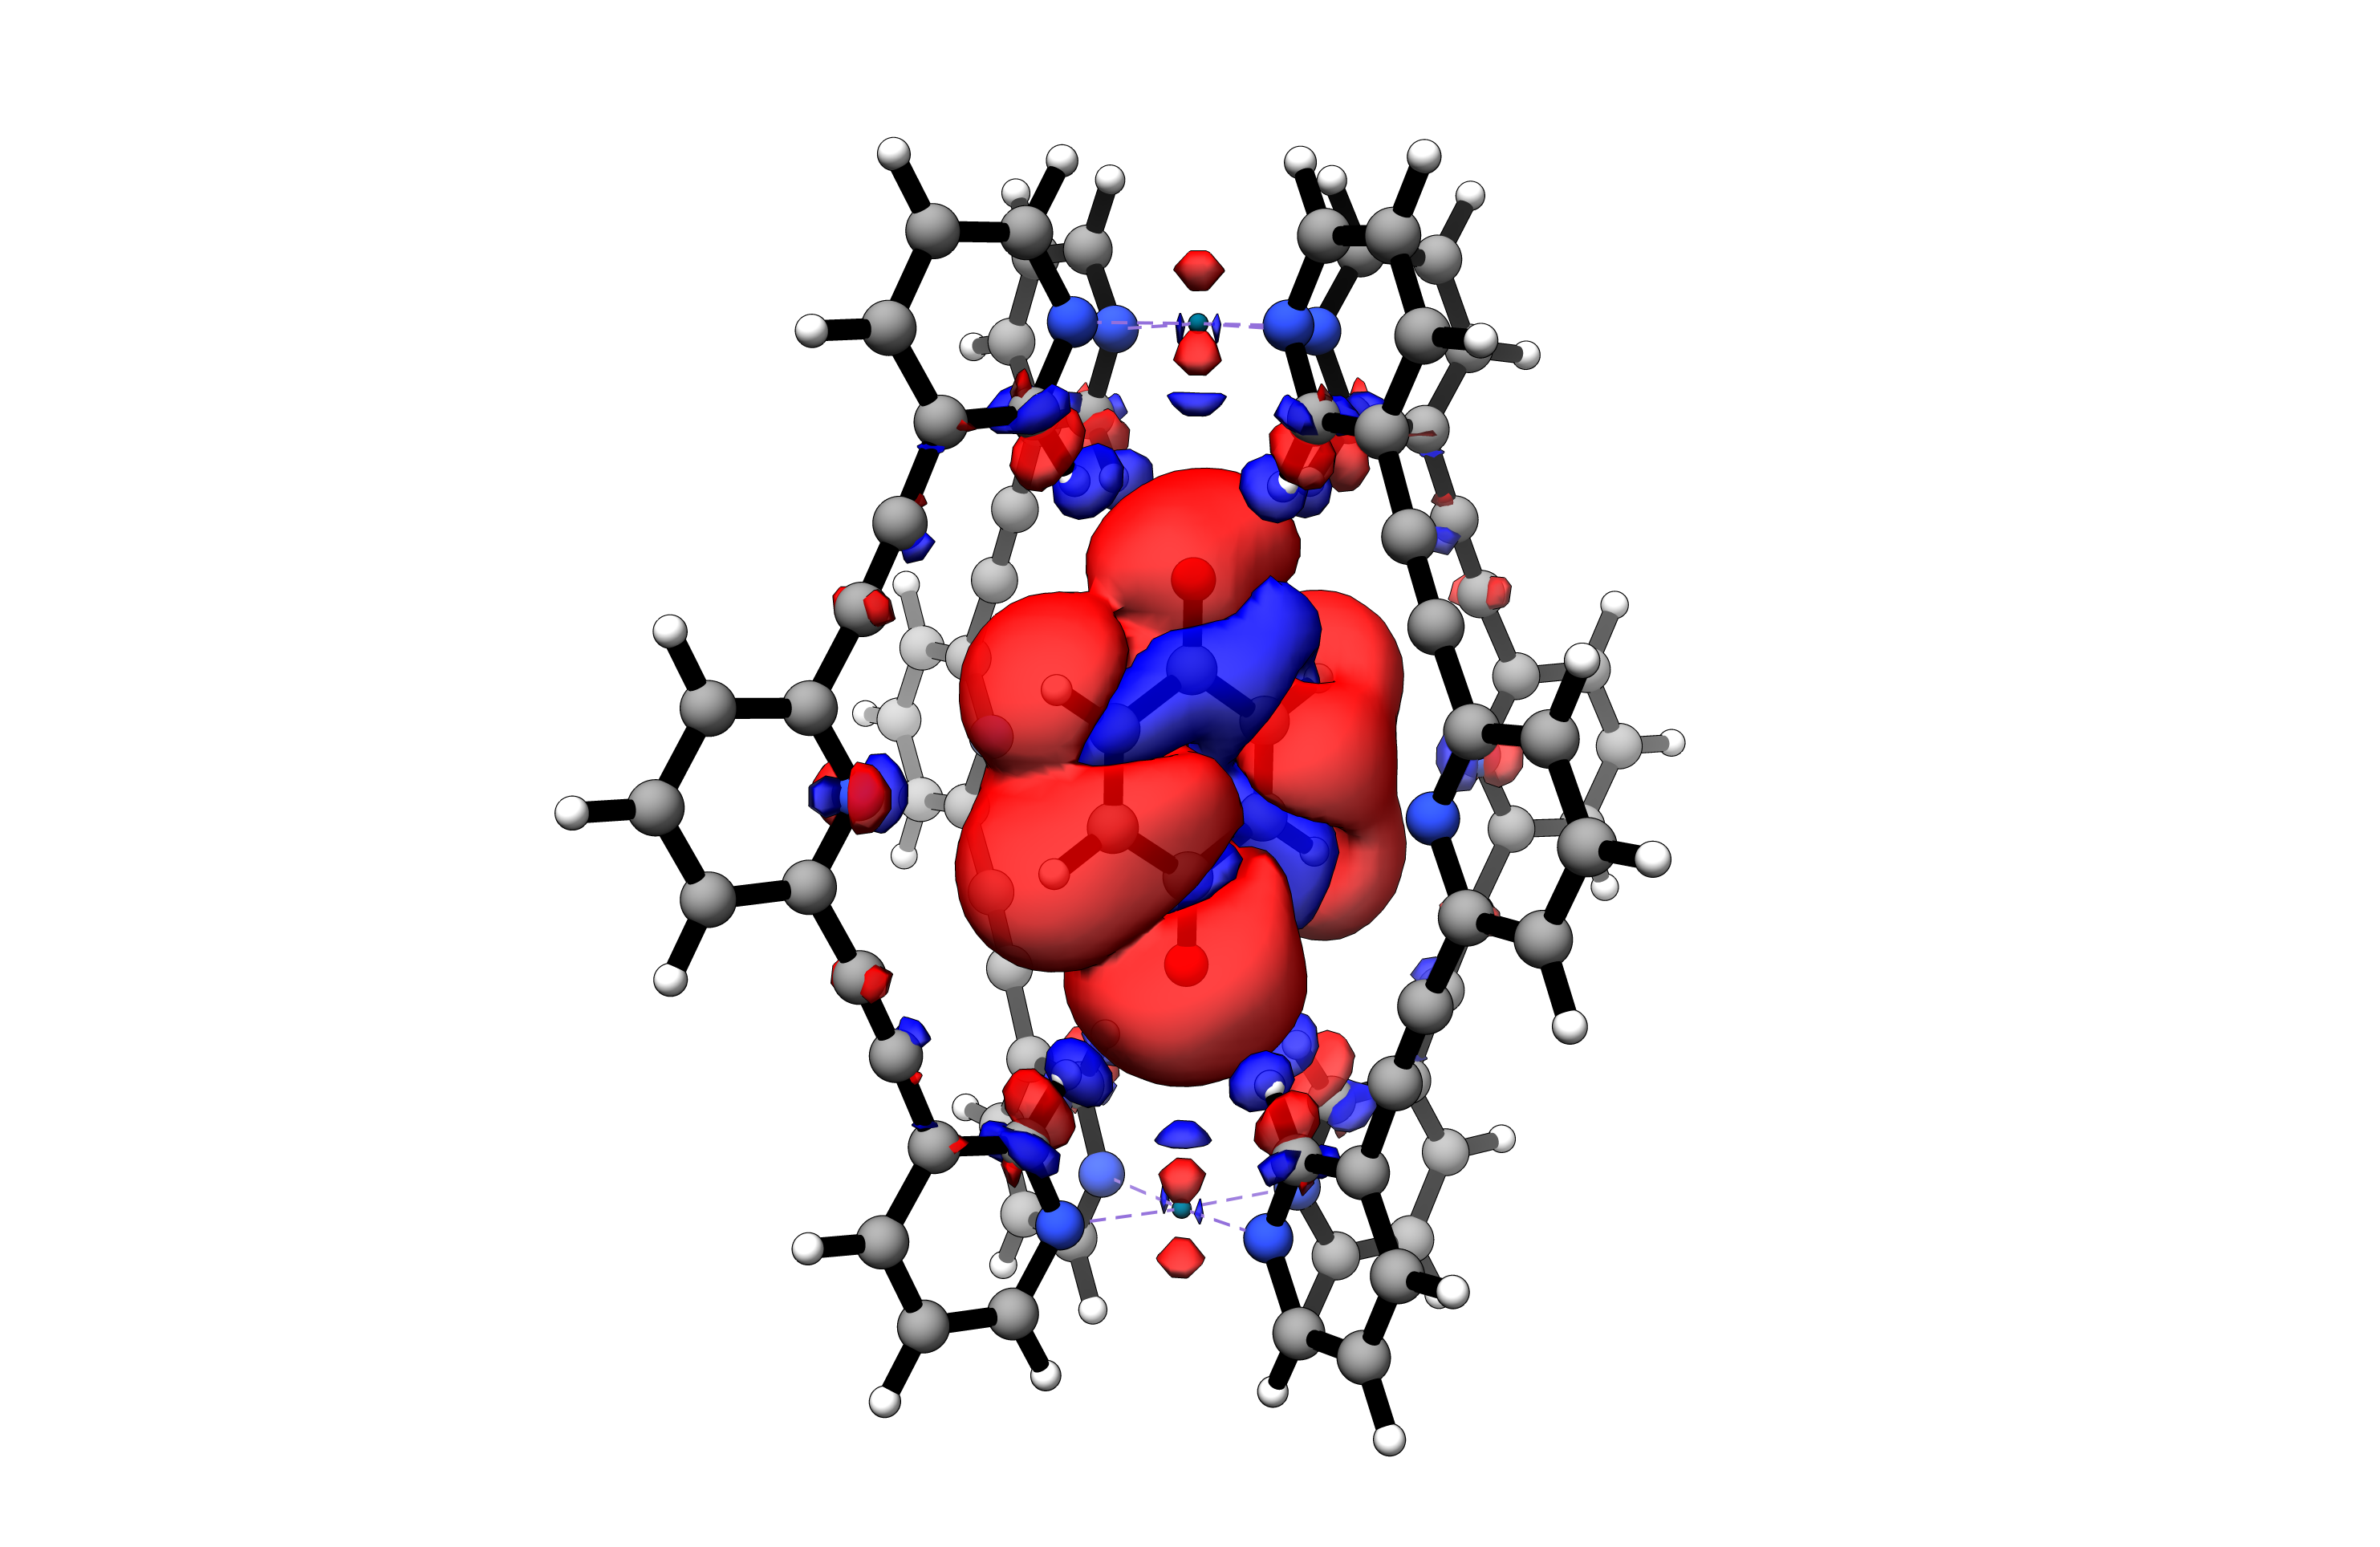
\includegraphics[width=\textwidth]{3/da//figs/figS24}
	\vspace{0.2cm}
	\hrule
	\caption{Electron density difference map for bq$\subset$C-2 showing regions depleted (red) and enhanced (blue) in electron density when the interaction between cage and substrate is activated. Density difference plotted at an isovalue of 0.001 au.}
	\label{fig::si_da_24}
\end{figure}


\begin{figure}[h!]
	\vspace{0.4cm}
	\centering
	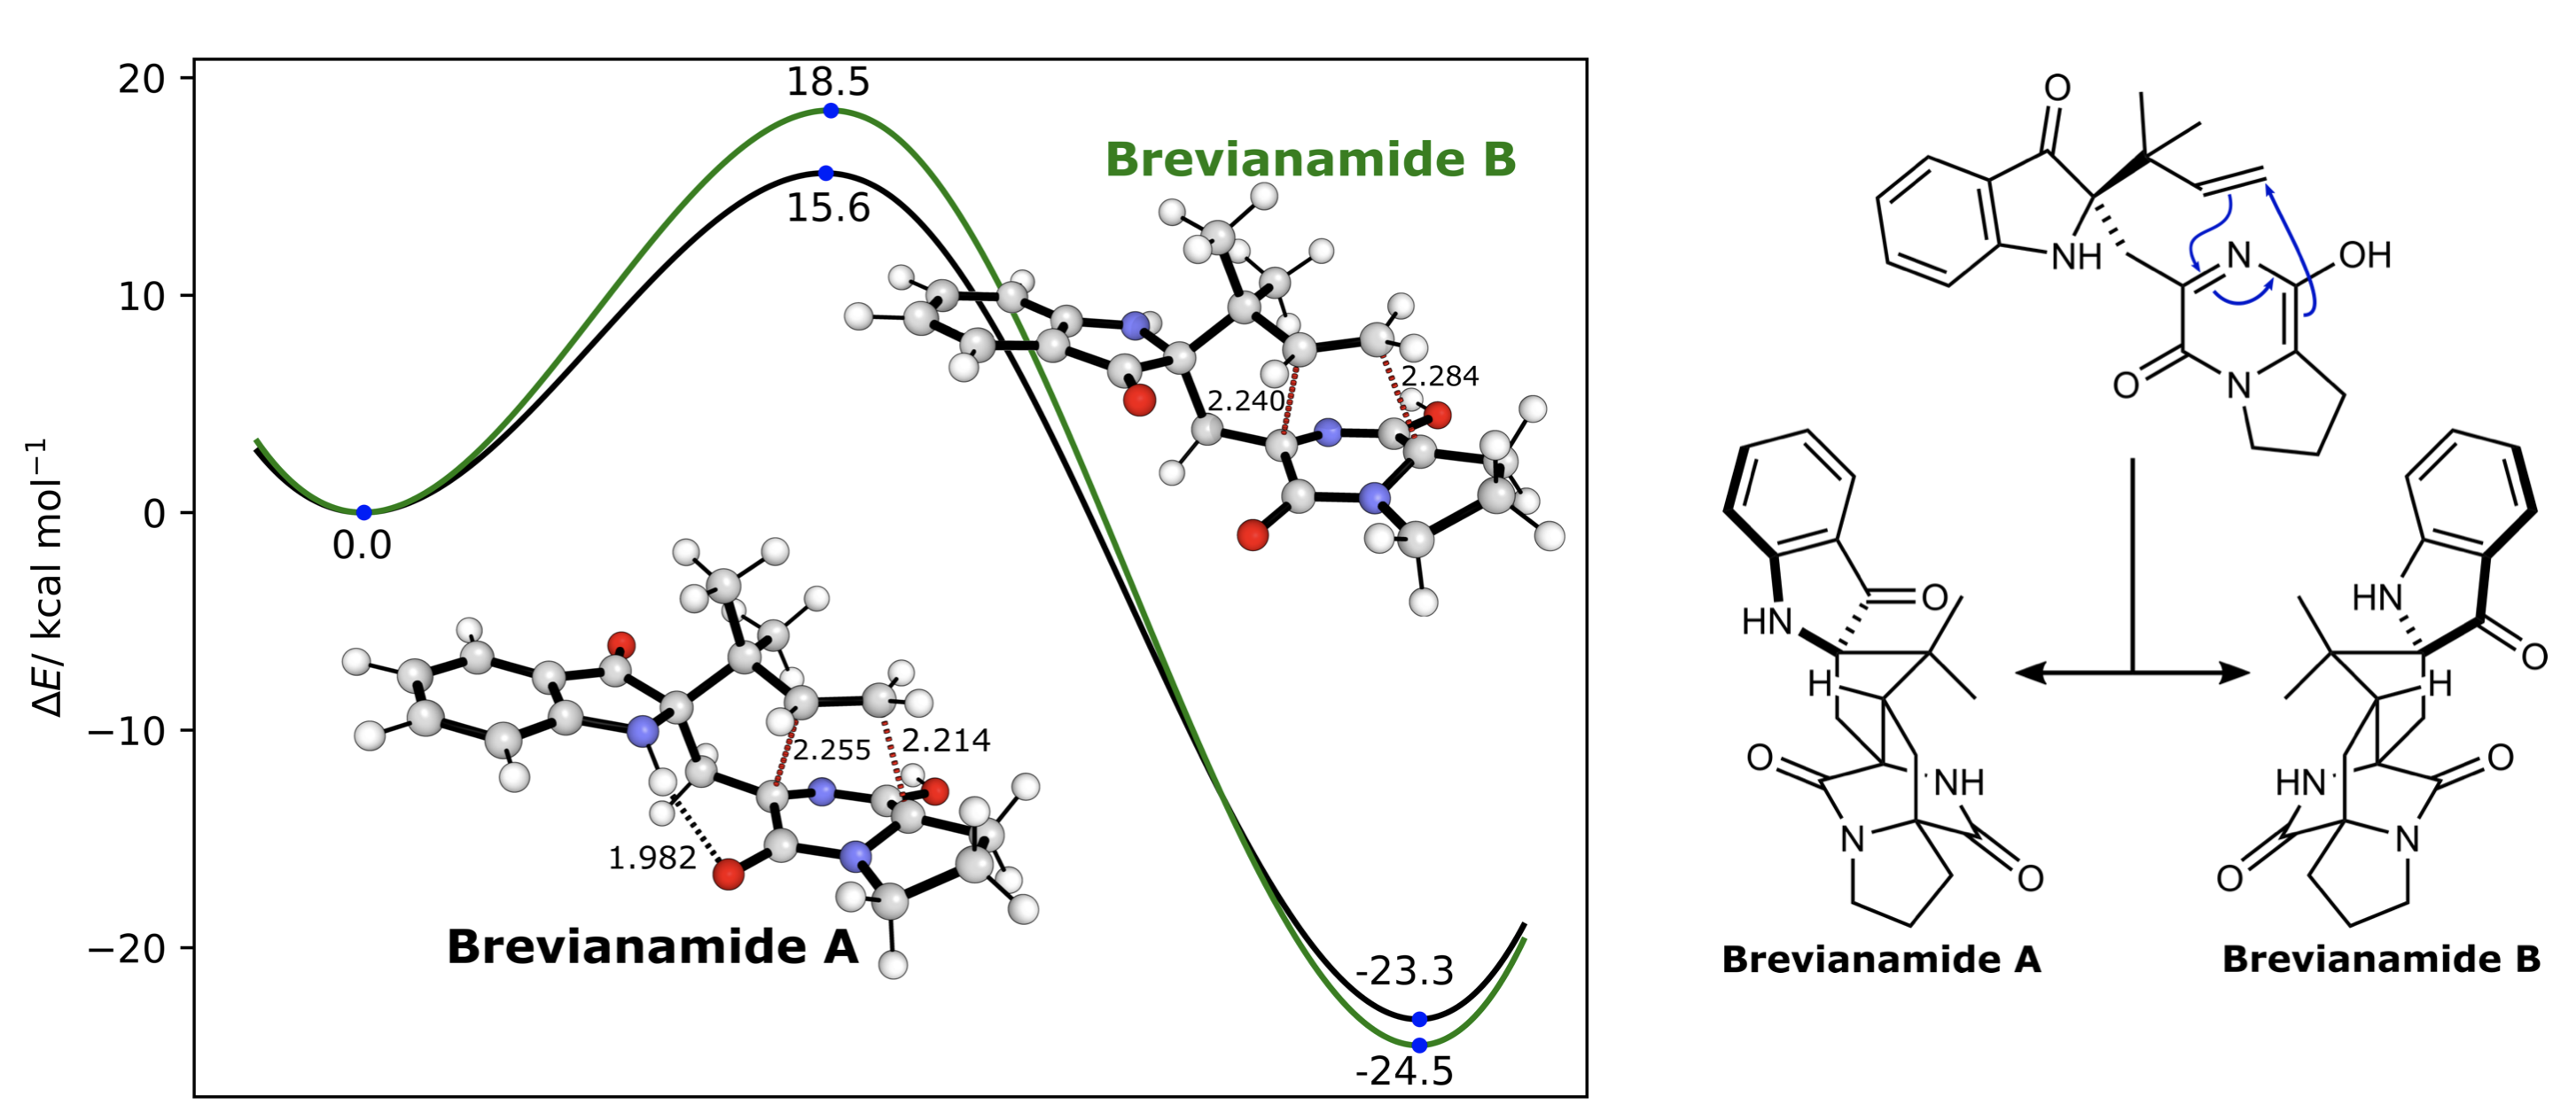
\includegraphics[width=\textwidth]{3/da//figs/figS25}
	\vspace{0.2cm}
	\hrule
	\caption{Reaction profile for the C-1/C-2 (orange/blue) encapsulated DA reaction between benzoquinone and isoprene.}
	\label{fig::si_da_25}
\end{figure}


For the full catalytic cycle presented in the manuscript the corresponding enthalpy and free energies are presented in Table \ref{table::si_da_20} and the corresponding structures in Figure \ref{fig::si_da_27}. Note that the free energies are much too positive, as the resting state is taken to be an empty cage, rather than occupied by a solvent molecule, thus there is a change in molecularity and a dominant translational entropy component. Energy differences balanced against DCM$\subset$C-2 are also presented in Table \ref{table::si_da_20}.

\begin{table}[h!]
	\def\arraystretch{1.7}
	\begin{tabularx}{\textwidth}{YYYYYYYY}
		\hline

		&&\multicolumn{3}{c}{Relative to empty cage}&	\multicolumn{3}{c}{Relative to DCM$\subset$C-X}	
\\
		Cage&	Species	&$\Delta E$	&$\Delta H$&	$\Delta G$&	$\Delta E$& $\Delta H$&	$\Delta G$	\\
				\hline
		&	INT0&	0.0	&0.0&	0.0&	0.0	&0.0&	0.0	
\\
		&	INT1&	-4.0&	-1.9&	9.8	&-10.2&	-9.7&	-7.9\\
		C-1 &TS1	&6.3&	9.9	&33.4&	0.0&	2.1	&15.7	
\\
		&	INT2&	-44.0&	-37.9&	-11.6&	-50.2&	-45.7&	-29.3	\\
		&	INT0 + product&	-45.7&	-41.7&	-28.7&	-45.7&	-41.7&	-28.7\\
		C-2	&INT0	&0.0&	0.0	&0.0&	0.0&	0.0	&0.0	\\
		&	INT1&	-3.3&	-0.5&	10.7&	-7.3&	-5.4&	-5.7	\\
		&	TS1	&1.1&	4.9	&29.6&	-2.9&	0.0	&13.1	
\\
		&	INT2&	-48.2&	-41.4&	-16.6&	-52.2&	-46.2&	-33.0	
\\
		&	INT0 + product&	-45.7&	-41.7&	-28.7&	-45.7&	-41.7&	-28.7	
\\
		 Cage&	Species	& $\Delta E$	& $\Delta H$	&$\Delta G$	&$\Delta H^\ddagger$&	 $\Delta H^\ddagger$	&	$\Delta G^\ddagger_\text{expt}$
\\
			uncat&	TS1	&&&			9.9	&10.7&	23.5	&24.0
\\
		C-1&	TS1		&&&		10.2&	11.8&	23.6&	$>$.0
\\
		C-2	&TS1	&&&			4.4	&5.4&	18.8&	20.4
	\end{tabularx}
	\hrule
	\vspace{0.2cm}
	\caption{Energetics for the full cycle for the uncatalysed and catalysed endo-reaction between benzoquinone and isoprene in the presence of C-1 and C-2. All calculated at the SMD(DCM)-M06-2X/def2-TZVP//PBE0-D3BJ/def2-SVP level of theory. Free energies are in the 1 M standard state. Experimental data from in ref \cite{MartCentelles2018}.}
	\label{table::si_da_20}
\end{table}



\begin{figure}[h!]
	\vspace{0.4cm}
	\centering
	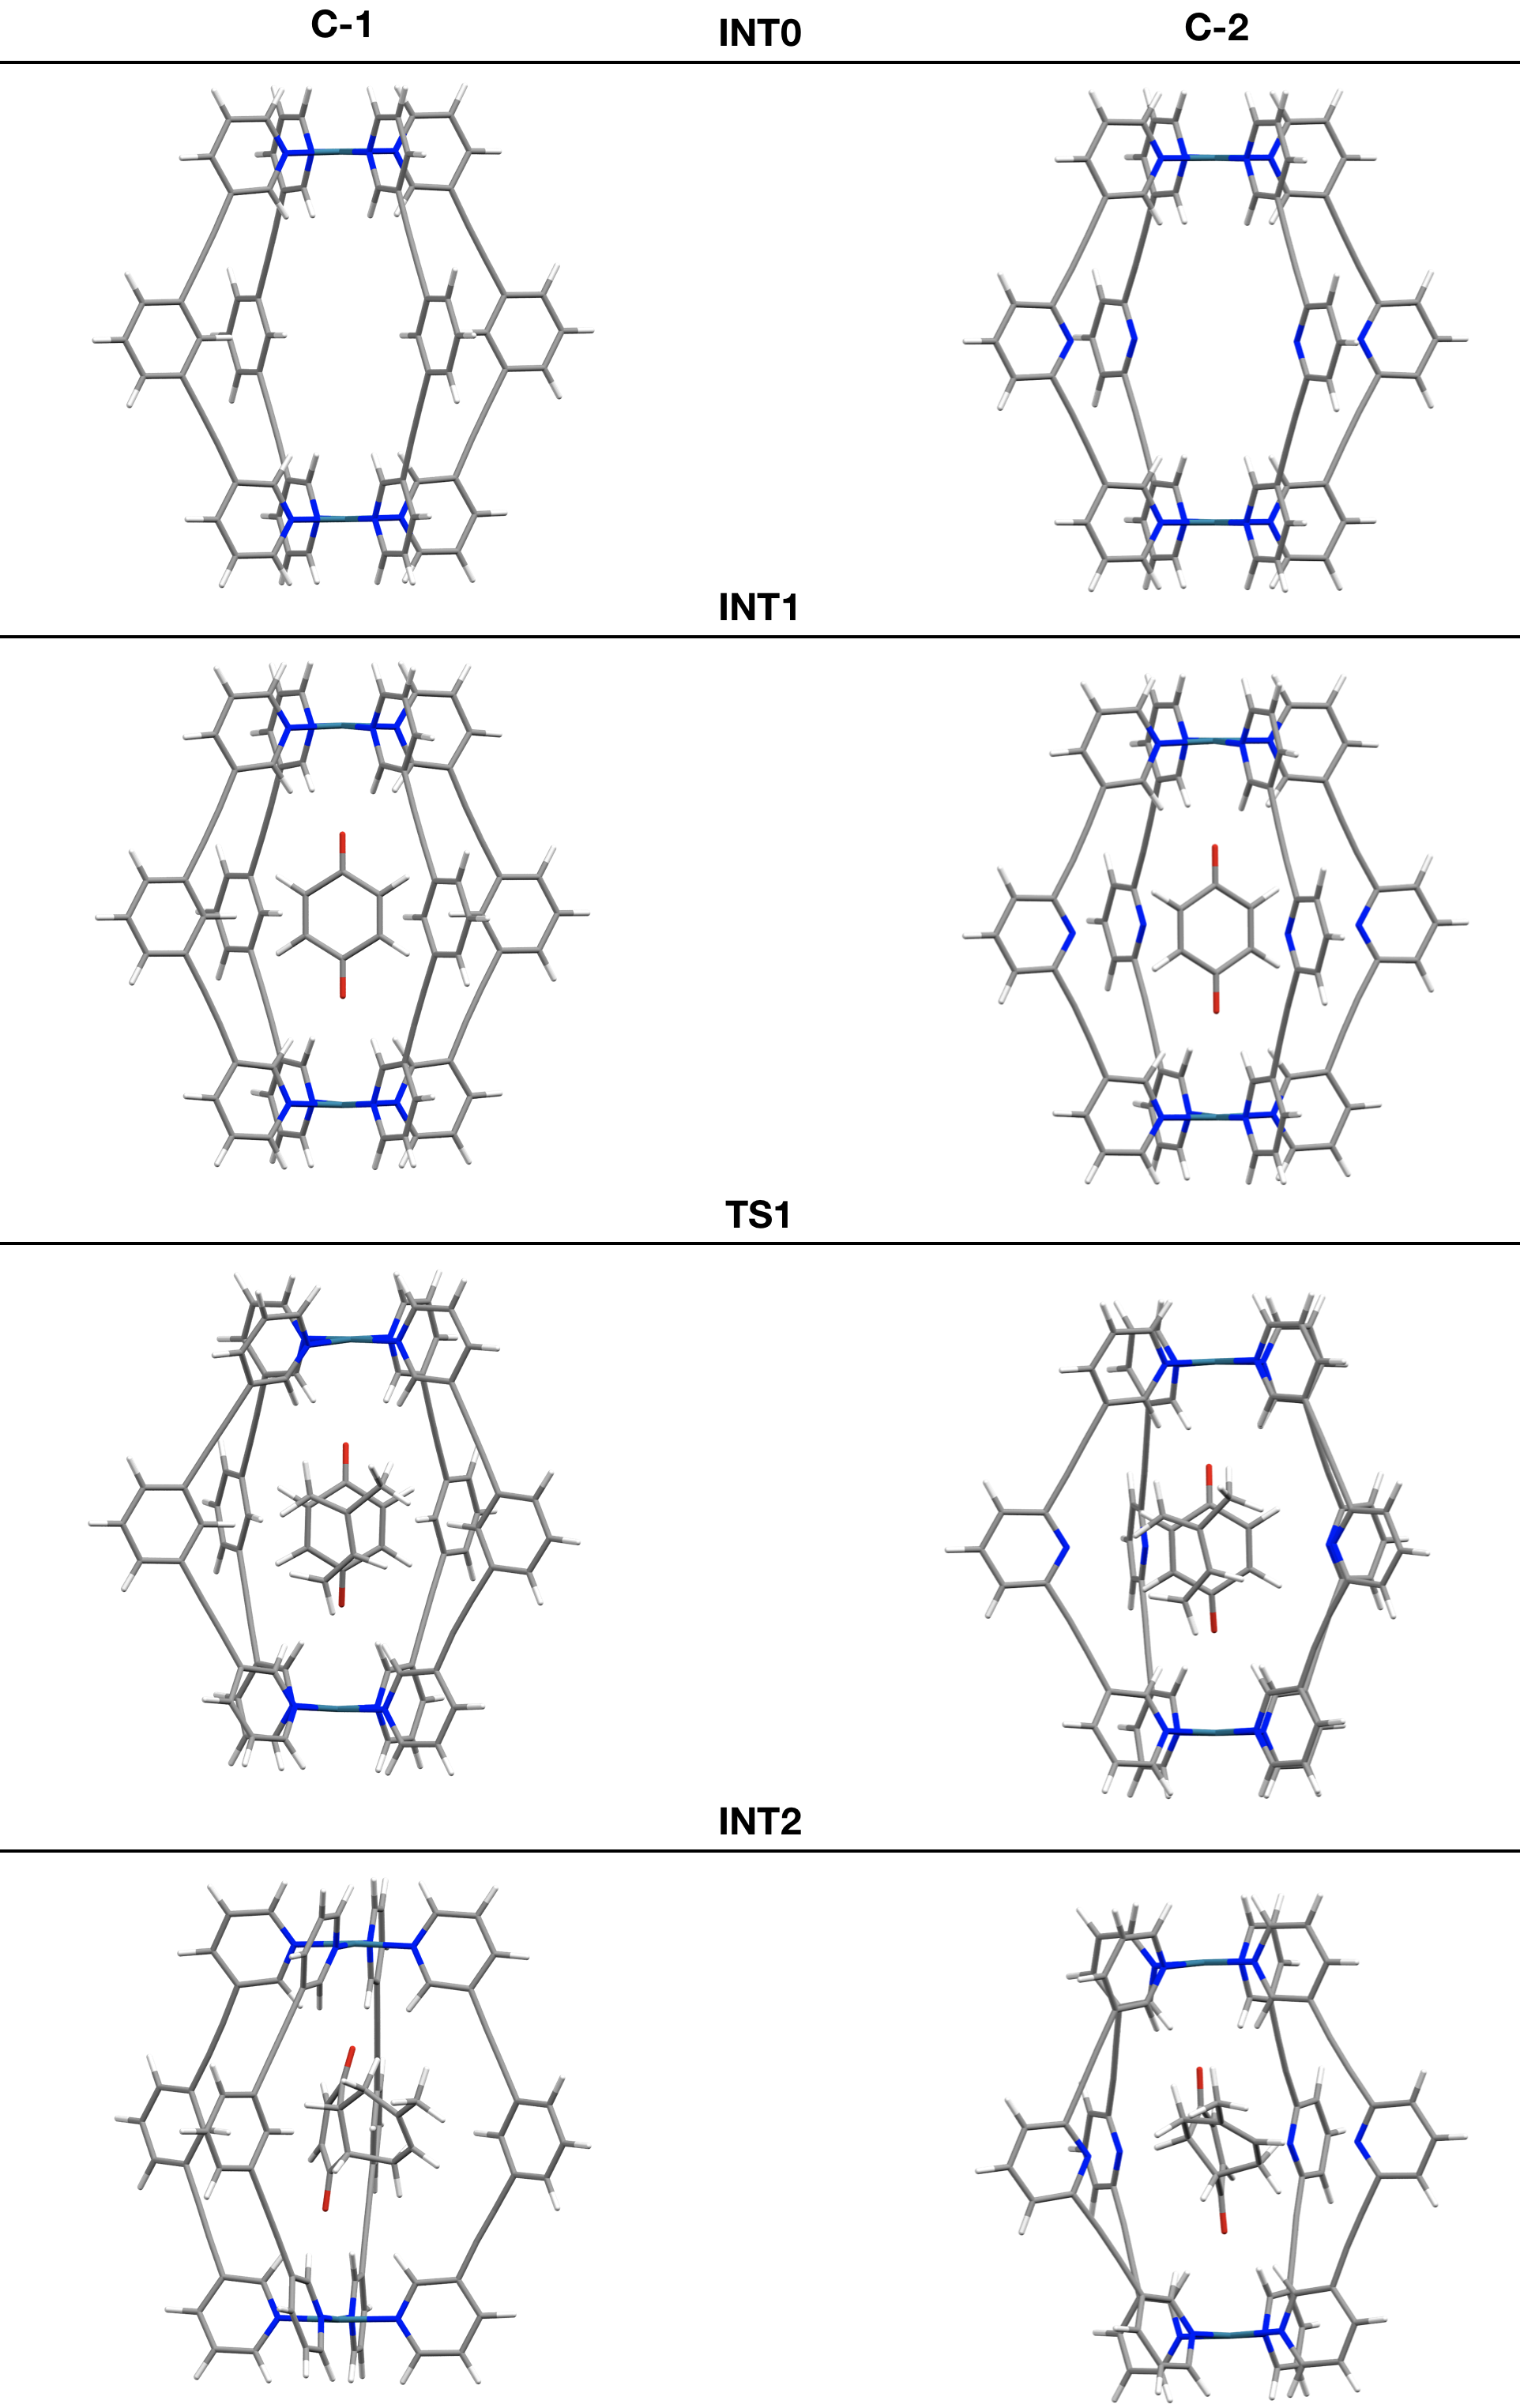
\includegraphics[width=13cm]{3/da//figs/figS27}
	\vspace{0.2cm}
	\hrule
	\caption{Optimized structures of the minima and TSs along the catalytic cycle at the at the PBE0-D3BJ/def2-SVP level of theory}
	\label{fig::si_da_27}
\end{figure}


\begin{figure}[h!]
	\vspace{0.4cm}
	\centering
	\includegraphics[width=12cm]{3/da//figs/figS28}
	\vspace{0.2cm}
	\hrule
	\caption{Distortion interaction analysis.}
	\label{fig::si_da_28}
\end{figure}


\begin{figure}[h!]
	\vspace{0.4cm}
	\centering
	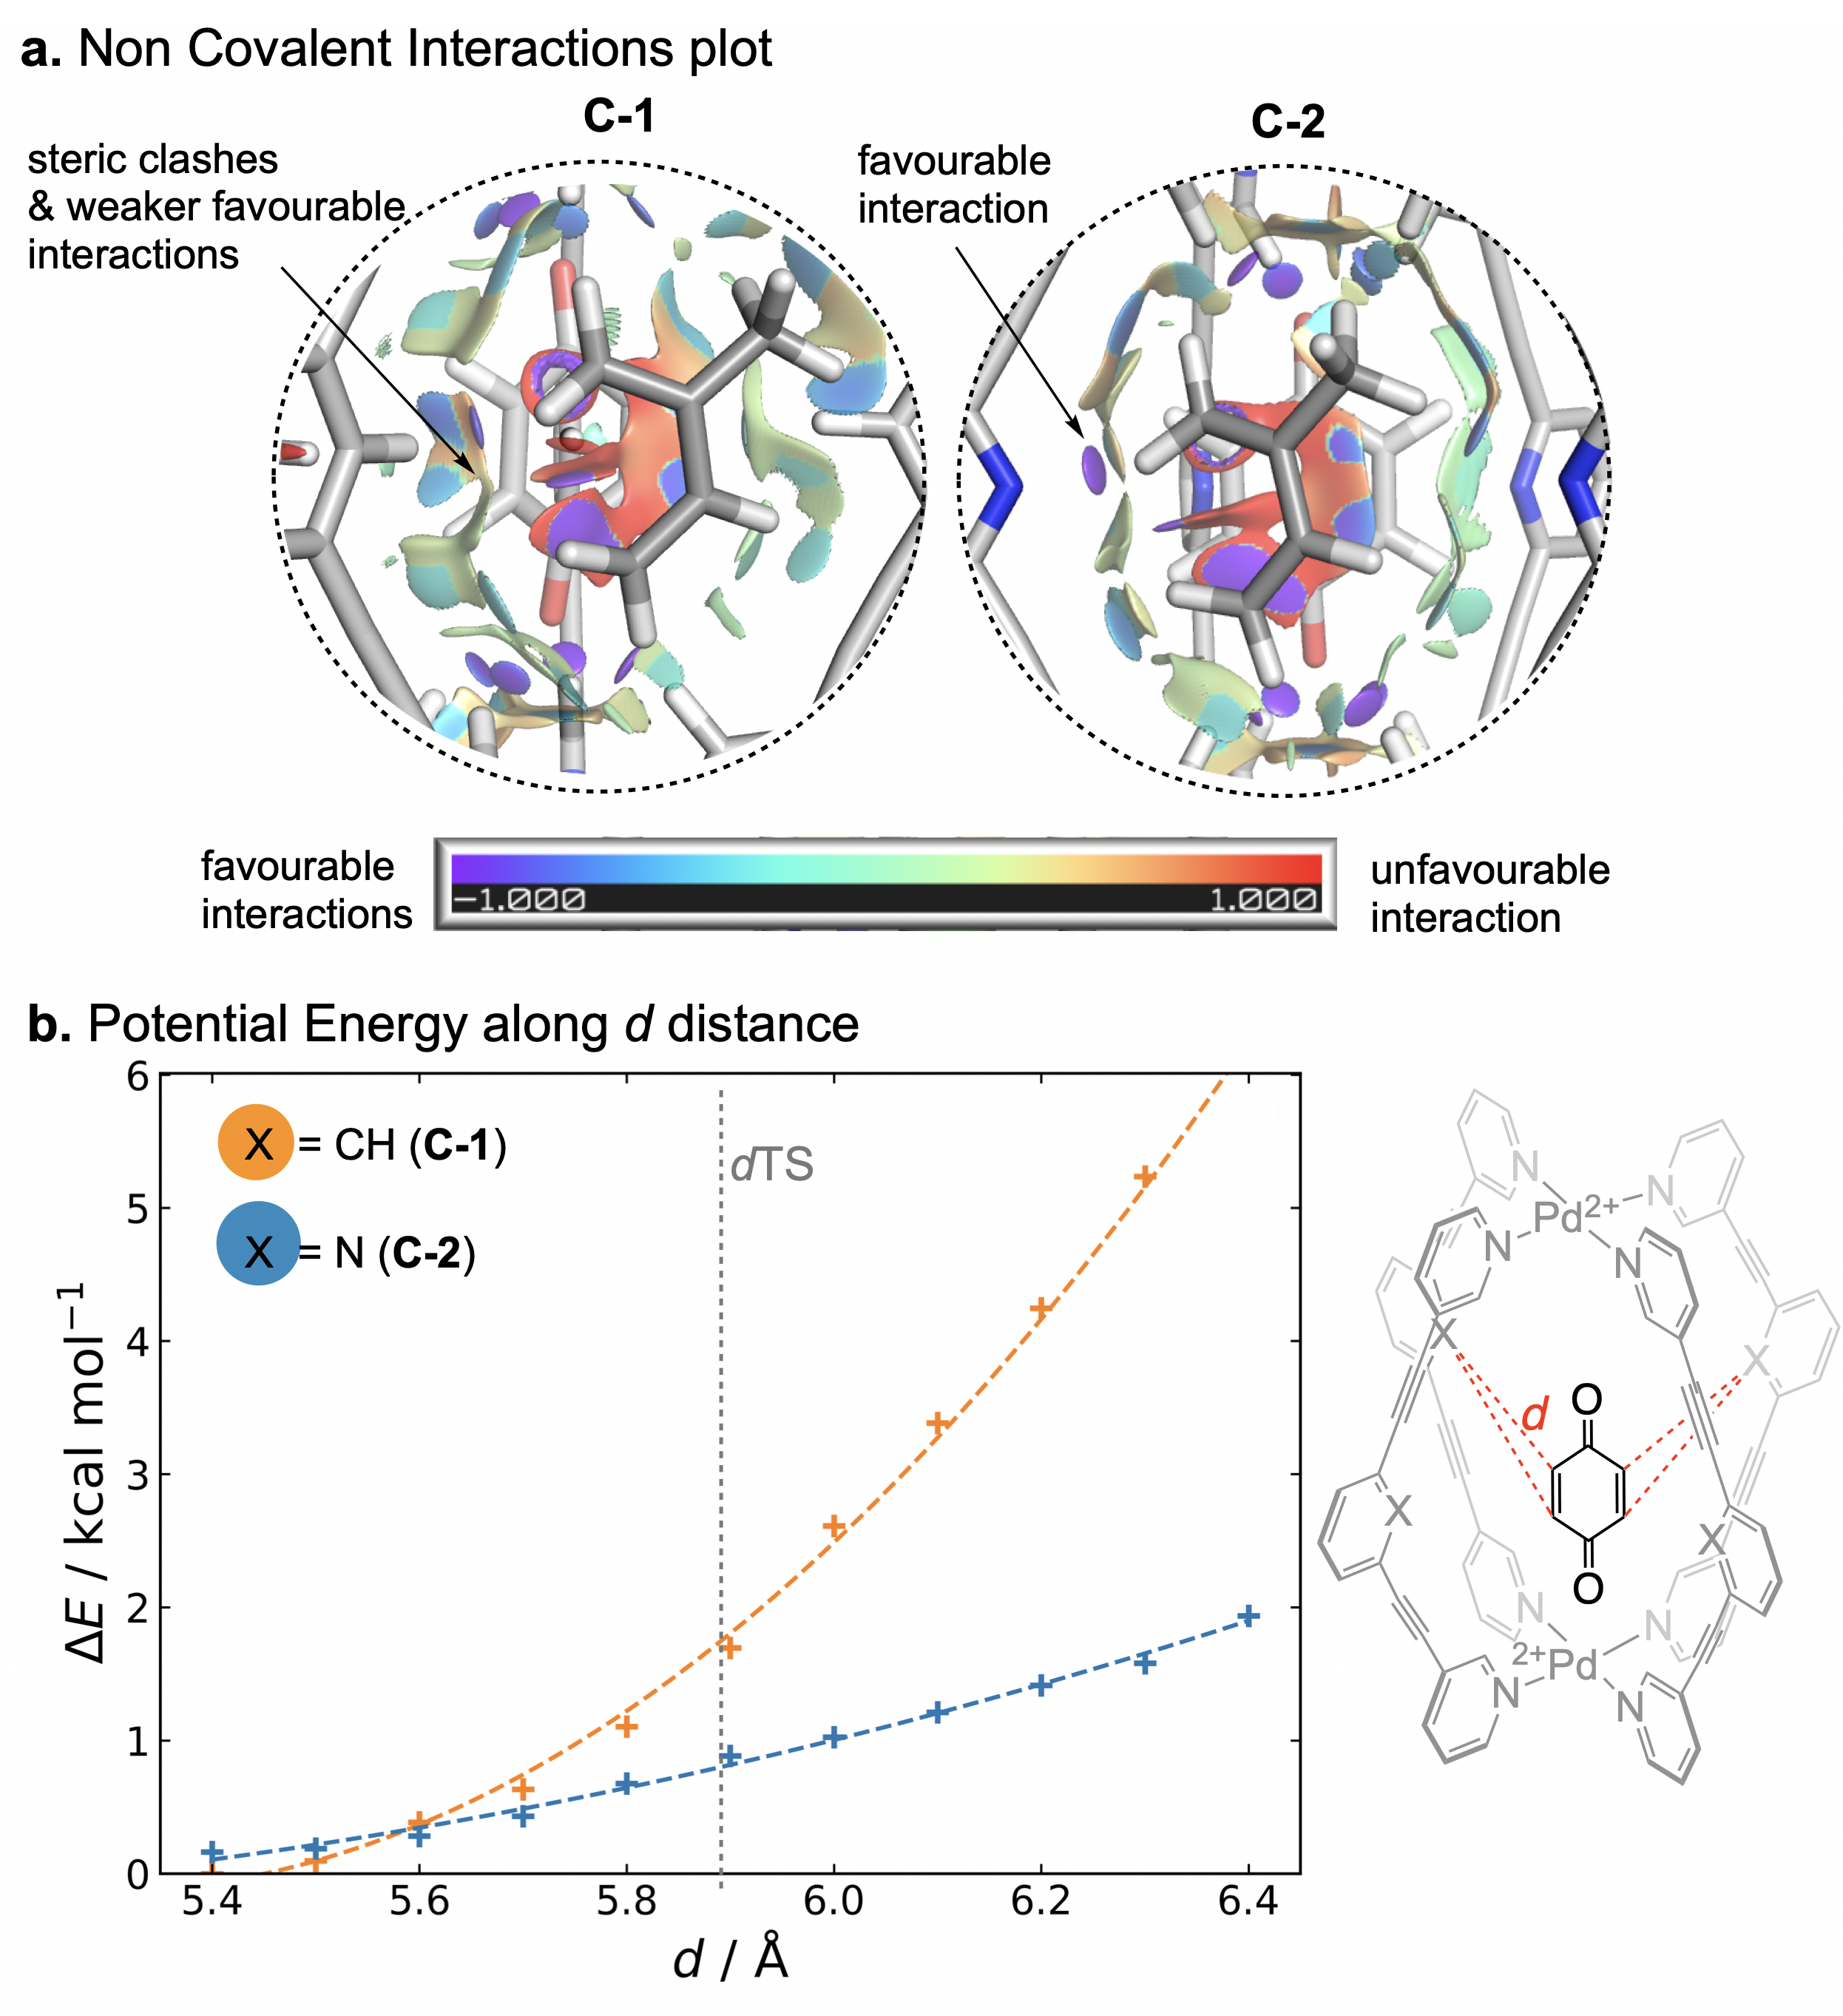
\includegraphics[width=12cm]{3/da//figs/figS29}
	\vspace{0.2cm}
	\hrule
	\caption{(a) Non-covalent interaction (NCI) isosurface (0.05 au) at the TS geometry for C-1 and C-2. An identifiable CH$\cdots$N interaction (purple circles) between the CH group of the diene and the catalyst nitrogen is observed in C-2. NCI calculated at the PBE0-D3BJ/def2-SVP level of theory. (b) Potential energy as a function of distance from 2 rearmost X (C/N) atoms to C$_\alpha$s on bq calculated at the PBE0-D3BJ/def2-SVP level of theory. Distance at the TS is indicated with a vertical grey line.}
	\label{fig::si_da_29}
\end{figure}



\begin{figure}[h!]
	\vspace{0.4cm}
	\centering
	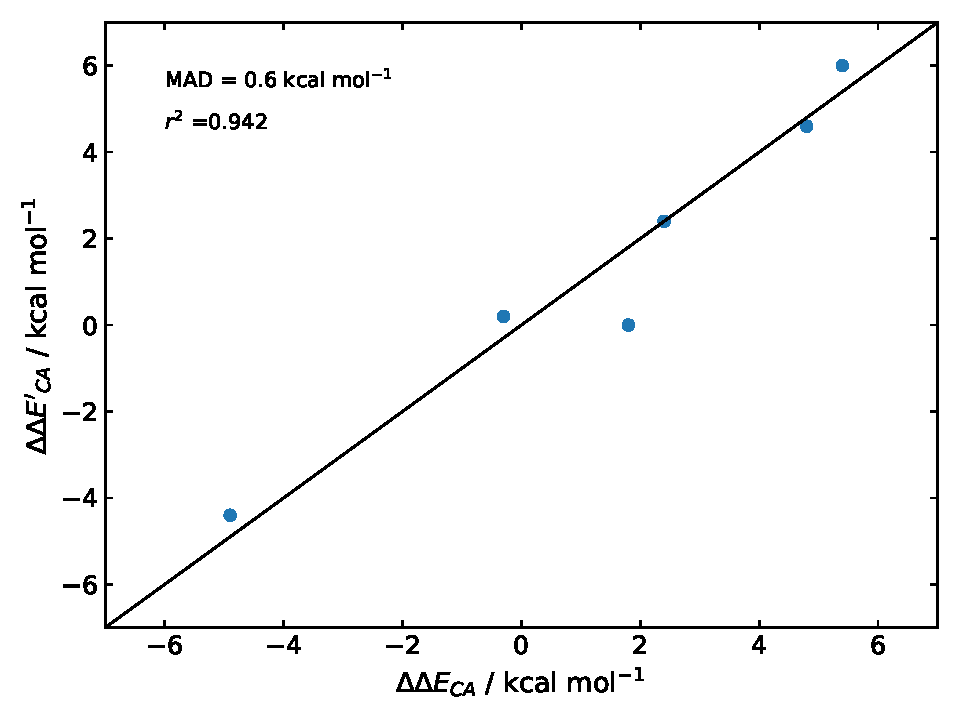
\includegraphics[width=10cm]{3/da//figs/figS30}
	\vspace{0.2cm}
	\hrule
	\caption{Calculated catalytic activity ($\Delta\Delta E_\text{CA} = \Delta E^\ddagger_\text{uncat} - E^\ddagger_\text{cat}$) using fully characterised transition states ($\Delta\Delta E_\text{CA}$) and transition state analogies ($\Delta\Delta E'_\text{CA}$).}
	\label{fig::si_da_30}
\end{figure}


\clearpage
\end{document}
